%%%%%%%%%%%%%%%%%%%%%%%%%%%%%%%%%%%%%%%%%
% Masters/Doctoral Thesis 
% LaTeX Template
% Version 2.5 (27/8/17)
%
% This template was downloaded from:
% http://www.LaTeXTemplates.com
%
% Version 2.x major modifications by:
% Vel (vel@latextemplates.com)
%
% This template is based on a template by:
% Steve Gunn (http://users.ecs.soton.ac.uk/srg/softwaretools/document/templates/)
% Sunil Patel (http://www.sunilpatel.co.uk/thesis-template/)
%
% Template license:
% CC BY-NC-SA 3.0 (http://creativecommons.org/licenses/by-nc-sa/3.0/)
%
%%%%%%%%%%%%%%%%%%%%%%%%%%%%%%%%%%%%%%%%%

%----------------------------------------------------------------------------------------
%	PACKAGES AND OTHER DOCUMENT CONFIGURATIONS
%----------------------------------------------------------------------------------------

\documentclass[
11pt, % The default document font size, options: 10pt, 11pt, 12pt
%oneside, % Two side (alternating margins) for binding by default, uncomment to switch to one side
spanish, % ngerman for German
singlespacing, % Single line spacing, alternatives: onehalfspacing or doublespacing
%draft, % Uncomment to enable draft mode (no pictures, no links, overfull hboxes indicated)
%nolistspacing, % If the document is onehalfspacing or doublespacing, uncomment this to set spacing in lists to single
%liststotoc, % Uncomment to add the list of figures/tables/etc to the table of contents
%toctotoc, % Uncomment to add the main table of contents to the table of contents
%parskip, % Uncomment to add space between paragraphs
%nohyperref, % Uncomment to not load the hyperref package
headsepline, % Uncomment to get a line under the header
%chapterinoneline, % Uncomment to place the chapter title next to the number on one line
%consistentlayout, % Uncomment to change the layout of the declaration, abstract and acknowledgements pages to match the default layout
]{MastersDoctoralThesis} % The class file specifying the document structure

\usepackage[utf8]{inputenc} % Required for inputting international characters
\usepackage[T1]{fontenc} % Output font encoding for international characters

\usepackage{mathpazo} % Use the Palatino font by default

% \usepackage[backend=bibtex,style=authoryear,natbib=true]{biblatex} % Use the bibtex backend with the authoryear citation style (which resembles APA)
\usepackage[
backend=biber,
bibencoding=utf8,
style=apa,
citestyle=authoryear,
sorting=nyt,
doi=false,
eprint=false,
natbib=true, % agrego MP
uniquename=false,
language=spanish
]{biblatex}
\DefineBibliographyStrings{spanish}{andothers = {et\addabbrvspace al\adddot}}

\addbibresource{bibliography.bib} % The filename of the bibliography

\usepackage[autostyle=true]{csquotes} % Required to generate language-dependent quotes in the bibliography
\usepackage{amsmath}
\usepackage{mathtools}
\usepackage{empheq}
\usepackage{amsfonts}
\usepackage{enumitem}
\usepackage{nameref, hyperref}
\usepackage{tikz}
\usetikzlibrary{shapes,arrows,calc,positioning}
\usepackage[ruled]{algorithm2e}
\usepackage[font=footnotesize,labelfont=bf]{caption}
\usepackage{soul}
\graphicspath{{./figs}}

%----------------------------------------------------------------------------------------
%	MACROS
%----------------------------------------------------------------------------------------

% Commands
\renewcommand{\v}[1]{\ensuremath{\mathbf{#1}}}
\newcommand{\gv}[1]{\ensuremath{\mbox{\boldmath$ #1 $}}}
\DeclareMathOperator*{\argmax}{argmax}
\DeclareMathOperator*{\argmin}{argmin}

% Revisions
\newcommand{\ma}[1]{\textcolor{red}{#1}}
\newcommand{\tjc}[1]{\textcolor{blue}{#1}}
\newcommand{\me}[1]{\st{#1}}

%----------------------------------------------------------------------------------------
%	MARGIN SETTINGS
%----------------------------------------------------------------------------------------

\geometry{
	paper=a4paper, % Change to letterpaper for US letter
	inner=2.5cm, % Inner margin
	outer=3.8cm, % Outer margin
	bindingoffset=.5cm, % Binding offset
	top=1.5cm, % Top margin
	bottom=1.5cm, % Bottom margin
	%showframe, % Uncomment to show how the type block is set on the page
}

%----------------------------------------------------------------------------------------
%	THESIS INFORMATION
%----------------------------------------------------------------------------------------

\thesistitle{Tratamiento de errores en asimilación de datos por ensambles: una aplicación en modelos epidemiológicos} % Your thesis title, this is used in the title and abstract, print it elsewhere with \ttitle
\supervisor{Manuel \textsc{Pulido}} % Your supervisor's name, this is used in the title page, print it elsewhere with \supname
\examiner{} % Your examiner's name, this is not currently used anywhere in the template, print it elsewhere with \examname
\degree{} % Your degree name, this is used in the title page and abstract, print it elsewhere with \degreename
\author{Tadeo Javier \textsc{Cocucci}} % Your name, this is used in the title page and abstract, print it elsewhere with \authorname
\addresses{} % Your address, this is not currently used anywhere in the template, print it elsewhere with \addressname

\subject{Ciencias de la Computación} % Your subject area, this is not currently used anywhere in the template, print it elsewhere with \subjectname
\keywords{asimilación de datos, modelos basados en agentes, algoritmo EM, epidemiología} % Keywords for your thesis, this is not currently used anywhere in the template, print it elsewhere with \keywordnames
\university{\href{https://www.unc.edu.ar/}{Universidad Nacional de Córdoba}} % Your university's name and URL, this is used in the title page and abstract, print it elsewhere with \univname
\department{\href{https://cs.famaf.unc.edu.ar/}{Sección de Ciencias de la Computación}} % Your department's name and URL, this is used in the title page and abstract, print it elsewhere with \deptname
\group{} % Your research group's name and URL, this is used in the title page, print it elsewhere with \groupname
\faculty{\href{http://www.famaf.unc.edu.ar/}{Facultad de Matemática, Astronomía, Física y Computación}} % Your faculty's name and URL, this is used in the title page and abstract, print it elsewhere with \facname

\AtBeginDocument{
\hypersetup{pdftitle=\ttitle} % Set the PDF's title to your title
\hypersetup{pdfauthor=\authorname} % Set the PDF's author to your name
\hypersetup{pdfkeywords=\keywordnames} % Set the PDF's keywords to your keywords
}

%----------------------------------------------------------------------------------------
%	DOCUMENT
%----------------------------------------------------------------------------------------

\begin{document}

\frontmatter % Use roman page numbering style (i, ii, iii, iv...) for the pre-content pages

\pagestyle{plain} % Default to the plain heading style until the thesis style is called for the body content

%----------------------------------------------------------------------------------------
%	TITLE PAGE
%----------------------------------------------------------------------------------------

\begin{titlepage}
    \begin{center}
    
    \vspace*{.06\textheight}
    {\scshape\LARGE \univname\par}\vspace{1.5cm} % University name
    \textsc{\Large Tesis Doctoral}\\[0.5cm] % Thesis type
    
    \HRule \\[0.4cm] % Horizontal line
    {\huge \bfseries \ttitle\par}\vspace{0.4cm} % Thesis title
    \HRule \\[1.5cm] % Horizontal line
     
    \begin{minipage}[t]{0.4\textwidth}
    \begin{flushleft} \large
    \emph{Autor:}\\
    \authorname % Author name
    \end{flushleft}
    \end{minipage}
    \begin{minipage}[t]{0.4\textwidth}
    \begin{flushright} \large
    \emph{Director:} \\
    \supname
    \end{flushright}
    \end{minipage}\\[3cm]
     
    \vfill
    
    % \large \textit{A thesis submitted in fulfillment of the requirements\\ for the degree of \degreename}\\[0.3cm] % University requirement text
    % \textit{in the}\\[0.4cm]
    % \groupname\\\deptname\\[2cm] % Research group name and department name
     
    \vfill
    
    {\large \today}\\[4cm] % Date
    %\includegraphics{Logo} % University/department logo - uncomment to place it
     
    \vfill
    \end{center}
\end{titlepage}

%----------------------------------------------------------------------------------------
%	ABSTRACT PAGE
%----------------------------------------------------------------------------------------

\begin{abstract}
    \addchaptertocentry{Resumen} % Add the abstract to the table of contents
    En este trabajo abordamos uno de los desafíos principales dentro de la disciplina de la asimilación de datos: la especificación de los las incertezas inherentes al modelo y a las observaciones en los sistemas parcialmente observados donde se aplican típicamente las técnicas de asimilación. Para ello presentamos el problema de asimilación de datos desde una perspectiva Bayesiana y los métodos más relevantes con especial énfasis en las técnicas basadas en ensambles. Además explicamos el efecto de los errores de modelo y observacionales sobre la performance de la asimilación de datos y las estrategias que se suelen usar para estimarlos. 
    Proponemos un método de inferencia de estos errores basado en el algoritmo EM y lo evaluamos experimentalmente. A diferencia de las implementaciones clásicas del EM, nuestra versión incorpora observaciones una a una lo cual la hace especialmente adecuada para contextos de asimilación de datos secuencial. 

    Tomamos a la epidemiología como campo de aplicación de las técnicas desarrolladas y estudiamos la factibilidad de su aplicación en modelos epidemiológicos compartimentales clásicos. Adicionalmente abordamos la posibilidad del uso de métodos de asimilación de datos por ensambles en modelos epidemiológicos basados en agentes. Este es un enfoque novedoso al problema ya que suele tratarse con modelos dinámicos basados en ecuaciones diferenciales. Con estos aportes mostramos el potencial de la aplicación de técnicas de asimilación de datos para estimar parámetros, errores y variables de estado en sistemas epidemiológicos.

\end{abstract}

\begin{extraAbstract}
    \addchaptertocentry{Abstract} % Add the abstract to the table of contents

    This work deals with one of the main challenges in the data assimiladion framework: the specification of the inherent uncertanties of the model  and measurements in partially observed systems where data assimilation techniques are typically applied. To do this, we present the data assimilation problem from a Bayesian perspective and the most relevant methods with special emphasis on ensemble-based techniques. We also adress the effect of model and observational error on data assimilation performance and the strategies commonly used to estimate them. We propose a method to inferr on these errors which is based on the EM algorithm and we give an experimental assesment of it. In contrast with classical EM implementation, our version incorporates observations one by one which makes it specially suitable in the context of sequential data assimilation.

    We take epidemiology as the main field of application of the techniques developed and we sutdy the feasibility of using them with classical compartimental epidemiological models. Additionaly we survey the possibility of using ensamble-based data assimilation techniques with epidemiological agent-based models. This is a novel approach to the problem which is ussualy tackled with dynamic models based on differential equations. With these contributions we showcase the potential of applying data assimilation to estimate model parameters, errors and state variables in epidemiological systems.

\end{extraAbstract}

%----------------------------------------------------------------------------------------
%	ACKNOWLEDGEMENTS
%----------------------------------------------------------------------------------------

% \begin{acknowledgements}
    % \addchaptertocentry{\acknowledgementname} % Add the acknowledgements to the table of contents

% \end{acknowledgements}

%----------------------------------------------------------------------------------------
%	LIST OF CONTENTS/FIGURES/TABLES PAGES
%----------------------------------------------------------------------------------------

\tableofcontents % Prints the main table of contents

% \listoffigures % Prints the list of figures

% \listoftables % Prints the list of tables

%----------------------------------------------------------------------------------------
%	THESIS CONTENT - CHAPTERS
%----------------------------------------------------------------------------------------

\mainmatter % Begin numeric (1,2,3...) page numbering

\pagestyle{thesis} % Return the page headers back to the "thesis" style

% Include the chapters of the thesis as separate files from the Chapters folder
% Uncomment the lines as you write the chapters

\chapter{Introducción}
En esta tesis exploramos algunos de los desafíos asociados a la aplicación de técnicas de asimilación de datos basadas en ensambles sobre modelos epidemiológicos. Abordamos el problema de la especificación de la incerteza inherente al modelo y las observaciones tanto en un marco general de modelos parcialmente observados como para el caso específico de modelos epidemiológicos basados en ecuaciones diferenciales. Además estudiamos el potencial de utilizar técnicas de asimilación de datos en modelos basados en agentes.

La asimilación de datos comprende un conjunto de técnicas estadísticas que se utilizan para combinar dos fuentes de información distintas sobre el estado de un mismo sistema: pronósticos provenientes de modelos matemáticos y observaciones. La disciplina está fuertemente emparentada con la predicción numérica meteorológica pues gran parte de su desarrollo está orientada a esos fines \citep{Talagrand1987}. En esta área, se cuenta con modelos matemáticos y computacionales muy complejos y de alta dimensionalidad que informan sobre diversas variables de estado (por ejemplo, velocidad, temperatura o presión) en diferentes puntos de una grilla espacial potencialmente muy grande ($10^7 - 10^8$ dimensiones). Estos modelos se basan en leyes físicas (por ejemplo, las ecuaciones de Navier-Stokes que expresan la conservación del momento y de la masa en fluidos), y permiten obtener pronósticos. Por otro lado, se tiene otra fuente de información sobre el mismo sistema que consta de las observaciones de diversos instrumentos en estaciones meteorológicas o provenientes de satélites. Ambas fuentes de información son propensas a errores. El error de modelo que comprende nuestro conocimiento limitado de la dinámica del sistema, aproximaciones y errores numéricos. El error observacional incuye la incerteza propia de los instrumentos de medición y el error de representatividad que involucra como se relacionan las observaciones con el estado del sistema (más sobre esto en la Sección \ref{sec:model_obs_error}). La asimilación de datos apunta a encontrar una combinación ponderada entre estas fuentes de información, de manera que si sabemos que la incerteza del modelo es menor que la de los datos, la estimación resultante será más fiel al modelo y si por el contrario, las observaciones tienen menos error que el pronóstico la estimación será más próxima a los datos.

El filtro de Kalman \citep{Kalman1960, Kalman1961} ocupa un lugar central dentro de las técnicas de asimilación de datos pues es una metodología sencilla que ha sentado las bases para métodos más sofisticados. Este tipo de filtro lineal encontró aplicaciones relevantes en la determinación de órbitas satelitales, navegación de submarinos y aeronaves e incluso de misiones espaciales como la Apollo \citep{Jazwinski1970}. En este tipo de aplicaciones típicamente tenemos que con el fin de estimar la posición y velocidad se utiliza como modelo a las ecuaciones físicas de movimiento mientras que las observaciones provienen de los instrumentos de navegación. Una gran parte del desarrollo de técnicas de asimilación de datos proviene sin embargo del área de las geociencias donde se presentan otro tipo de desafíos como la alta dimensionalidad de los sistemas, observaciones menos precisas y modelos caóticos altamente no-lineales. Por ejemplo, el filtro de Kalman por ensambles \citep{Evensen1994} toma la idea original de Kalman incorpora la idea de representar distribuciones mediante muestras lo cual permite adaptar el problema a situaciones de no-linealidad. La familia de métodos por ensambles pudo competir con los más tradicionales métodos variacionales (3D-VAR y 4D-VAR) que formulan al problema como la minimización de una función de costo y que son utilizados en grandes centros meteorológicos \citep{Kalnay2007}. Otras técnicas más modernas han comenzado a ganar relevancia en el campo: notablemente los filtros de partículas que permiten la representación de distribuciones no Gaussianas han conformado otra gran familia de metodologías de creciente interés \citep{vanLeeuwen2019}. Muchas de las técnicas de asimilación de datos fueron desarrolladas inicialmente para resolver problemas asociados a la predicción numérica meteorológica pero el campo de apicación es mucho más diverso. Se utilizan, por ejemplo, para navegación aeorespacial \cite{Grewal2010}, predicción sobre reservorios petrolíferos \cite{Aanonsen2009}, oceanografía, detección de incendios forestales \citep{Mandel2008}, epidemiología \citep{Shaman2012}, entre otras. En el Capítulo \ref{chp:da} formulamos el problema de la asimilación de datos desde una perspectiva Bayesiana e introducimos las técnicas más relevantes para el desarrollo de nuestro trabajo. En \cite{Carrassi2018} se puede encontrar un buen panorama del estado del arte en cuanto a metodologías de asimilación de datos.

Actualmente el creciente interés en machine learning y los grandes avances en el área en las últimas décadas motivó interés en el intercambio entre esta área y la asimilación de datos. Por ejemplo, en \cite{Abarbanel2018} se plantea una interpretación de las redes neuronales en el contexto de  problemas de asimilación de datos dando una equivalencia entre agregar capas a la red neuronal con la resolución temporal en el problema de asimilación. Además también se señala la utilidad de algunas herramientas de asimilación para su aplicación en machine learning. En esta dirección \cite{Kovachki2019} propone el uso técnicas basadas en filtros de Kalman por ensambles para asistir el entrenamiento de modelos supervisados y semisupervisados de manera que se evita el uso de gradientes.

Como mencionamos anteriormente, la asimilación de datos tiene en cuenta la incerteza del modelo que genera los pronósticos del sistema tanto como la proveniente de las observaciones. Una especificación errónea de estas cantidades puede causar una performance subóptima de la inferencia pero es habitual que estos errores sean difíciles de identificar. Por lo tanto, existe una variedad de métodos para proveer estimaciones para el error observacional y de modelo \citep{Tandeo2020}. Estos incluyen metodologías basadas en momentos estadísticos y otras que apuntan a la maximización de la verosimilitud entre las cuales hacemos mención del algoritmo EM \citep{Dempster1977}, el cual puede ser implementado en el contexto de asimilación de datos con filtros de Kalman y en particular con filtros basados en ensambles \citep{Tandeo2015}. La implementación clásica del algoritmo EM toma un lote (\textit{batch}) de datos y los procesa a todos juntos para dar proveer estimaciones de los parámetros que codifican los errores. Esto trae una serie de inconvenientes a la hora de ser utilizado en sistemas de asimilación secuencial en los que los datos son producidos y procesados en tiempo real o casi real. El procesamiento por lotes (\textit{offline}) por un lado, fuerza a almacenar todo el conjunto de observaciones y por otro, cuando ingresa una observación no es en principio adaptable a incorporarla por lo que el proceso debe reiniciarse. Esta situación ha despertado interés en técnicas de inferencia \textit{online}, es decir que permitan actualizaciones con cada nueva observación y de manera que cada dato es procesado una única vez. En esta dirección se destaca la metodología desarrollada en \cite{Berry2013} la cual es basada en innovaciones (esto, a grandes rasgos significa que se basa en las diferencias entre pronósticos y observaciones) y que está específicamente diseñada para contextos de asimilación de datos. Por otro lado, luego del trabajo seminal de \cite{Neal1998} tenemos versiones \textit{online} del EM por \cite{Andrieu2003} y por Cappé \citep{Cappe2009,Cappe2011}.Estas sin embargo no están explícitamente diseñadas para ser acopladas a técnicas clásicas de asimilación de datos. Por el interés en metodologías de este tipo y su relevancia nos vimos motivados a desarrollar una versión \textit{online} del EM que se adapta a estrategias de asimilación de datos por ensambles. En el Capítulo \ref{chp:error_treatment} introducimos el problema de tratamiento de errores, discutimos algunas de las metodologías más conocidas y finalmente presentamos nuestro algoritmo EM \textit{online} con su deducción teórica y una evaluación experimental de su desempeño.

El marco en el que se suele aplicar la asimilación de datos es el de un sistema que evoluciona temporalmente y es parcialmente observado. A pesar de no ser una de las áreas típicas de aplicación, los sistemas epidemiológicos tienen estas características y pueden servise de las herramientas de la asimilación de datos. Desde comienzos del siglo pasado se han utilizado modelos matemáticos para estudiar las dinámicas de transmisión de enfermedades. Los populares modelos compartimentales basados en ecuaciones diferenciales \citep{Kermack1927} han sido adaptados a una gran diversidad de escenarios epidemiológicos permitiendo predicción de picos epidémicos, simulación de medidas de prevención y mitigación, estimación de parámetros, etc. Sin embargo, los ejemplos de aplicación de asimilación de datos sobre estos modelos no son tan abundantes como en otras áreas. Los trabajos de \cite{Ionides2006} y \cite{Shaman2012} marcaron un precedente en este sentido: en el primero se utilizan filtros de partículas y en el segundo filtro de Kalman por ensambles para un modelo de cólera y gripe respectivamente. Luego, con el advenimiento de la pandemia de COVID-19 este abordaje se hizo algo más popular (por ejemplo \cite{Evensen2020, Li2020}). A pesar de que la asimilación de dtos en estos sistemas comenzó a ser más popular, la estimación de errores observacionales y de modelo en estos trabajos es infrecuente. Esto motivó que  tomemos un modelo epidemiológico compartimental sencillo para COVID-19 como ejemplo de aplicación de nuestro algoritmo EM \textit{online} y con la motivación de estudiar el efecto de estos errores en sistemas epidemiológicos. En el Capítulo \ref{chp:epi_models} mostramos los resultados previamente introduciendo los elementos básicos del modelado epidemiológico y los antecedentes de inferencia estadística basada en asimilación de datos en este tipo de escenario.

Los modelos epidemiológicos compartimentales están típicamente representados mediante ecuaciones diferenciales y las técnicas de asimilación de datos son en general aplicadas a modelos dinánmicos con esta característica. Sin embargo, se han popularizado, en parte a las posiblidades que abre el aumento del poder de cómputo, los modelos basados en agentes. Estos, en lugar de tomar las variables de interés y representar su comportamiento mediante ecuaciones, simulan una población de individuos a través de un conjunto de reglas de interacción. El comportamiento global del sistema es entonces el resultado del comportamiento colectivo de la totalidad de los agentes. Este paradigma provee gran adaptabilidad y expresividad a estos modelos ya que permiten representar situaciones mediante reglas simples de interrelación entre individuos que pueden ser muy difíciles de reproducir mediante ecuacuiones diferenciales. Con la notable excepción del trabajo de \cite{Ward2016}, no existen en nuestro conocimiento aplicaciones de asimilación de datos sobre modelos de agentes. En el Capítulo \ref{chp:da_abms} damos un marco general de aplicación de asimilación de datos basada en ensambles para modelos basados en agentes y hacemos una evaluación experimental de la metodología sobre un modelo que desarrollamos en base a las características epidemiológicas del COVID-19.

Al momento de inicial el trabajo de este doctorado planificabamos trabajar con modelos de Dengue. Esta a enfermedad tiene la particularidad de que la transmisión no es persona a persona sino que es transmitida por vectores (en este caso mosquitos) y esto da lugar a modelos compartimentales interesantes como por ejemplo \cite{}. La motivación por estudiar la propagación del Dengue tiene que ver con el problema sanitario que significa en Argentina y continuaba el trabajo iniciado en mi tesis de Licenciatura en Matemática \citep{}. Sin embargo el surgimiento del COVID-19 dio lugar a que entendiblemente, el interés de la comunidad científica se concentre en esta enfermedad y que proliferen modelos y métodos de inferencia para intentar comprender mejor este fenómeno. Debido a esto y también por la gran disponibilidad de datos accesibles por el monitoreo de la pandemia, decidimos usar al COVID-19 como ejemplo de aplicación

\chapter{Asimilación de datos}

\section{Asimilación de datos como un problema de inferencia bayesiana}

La asimilación de datos busca hacer inferencia sobre variables de estado $\v x$ incorporando información observacional $\v y$. Si pensamos en la distribución de probabilidad de $\v x$, el objetivo será encontrar $p(\v x | \v y)$, la distribución \textit{a posteriori}. En este tipo de escenarios, es natural aplicar la regla de Bayes para obtener
\begin{align*}
    p(\v x | \v y) = \frac{p(\v y | \v x)p(\v x)}{p(\v y)}
\end{align*}
donde $p(\v y | \v x)$ es la verosimilitud, $p(\v x)$ es la distribución \textit{a priori} de las variables de estado y va a estar determinada por nuestro modelo de pronóstico, mientras que $p(\v y)$ puede ser vista como una constante de normalización. La verosimilitud se interpreta como una función de $\v x$ y nos informa cuán factible es que la observación $\v y$ haya sido producida por el estado $\v x$. La verosimilitud de $\v x$ habiéndose observado $\v y$ se suele denotar como $\mathcal{L}(\v x ; \v y)$ para enfatizar que no es una densidad de probabilidad y que es función de $\v x$. La verosimilitud va a estar determinada por el modelo observacional, que es la representación de cómo se obtiene un dato desde las variables de estado.

\subsection{State-space model}

Si consideramos que tenemos un proceso en el que las variables de estado evolucionan temporalmente, podemos denotar a un conjunto de realizaciones del proceso como $\v x_{0:t} = \v x_0, ..., \v x_t$ y, de manera similar, a las observaciones sobre ese proceso como $\v y_{1:t} = \v y_1, ..., \v y_t$. Las variables de estado evolucionan del tiempo $t$ al $t+1$ a través de un modelo $\mathcal{M}_t$ y a su vez, el modelo observacional $\mathcal{H}_t$ es el que representa como se obtiene la observación $\v y_t$ del estado $\v x_t$: 
\begin{align}
    \v x_t &= \mathcal M_{t} (\v x_{t-1}, \gv\eta_t), \label{eq:transition} \\
    \v y_t &= \mathcal H_{t} (\v x_t, \gv\nu_t). \label{eq:observation}
\end{align}
En estas ecuaciones introducimos $\gv\eta_t$ y $\gv\nu_t$ como las componentes estocásticas que dan cuenta del error de modelo y observacional respectivamente.

Notemos además que la ecuación \ref{eq:transition} determina una probabilidad de transición $p(\v x_t | \v x_{t-1})$ y la ecuación \ref{eq:observation} define una verosimilitud observacional $\mathcal{L}_t(\v x_t ; \v y_t) = p(\v y_t | \v x_t)$. Es una convención en asimilación de datos considerar a las variables de estado idexadas desde el $0$ y a las observaciones desde el $1$. De esta manera se asume que $\v x_0$ no es observado. Si además suponemos que el estado inicial responde a una distribución, i.e.,  $\v x_0 \sim p(\v x_0)$, podemos plantear al problema de la siguiente manera:
\begin{align}
    \v x_0 &\sim p(\v x_0) \\
    \v x_t | \v x_{t-1} &\sim p(\v x_t | \v x_{t-1}) \\
    \v y_t | \v x_t &\sim p(\v y_t | \v x_t)
\end{align}

Si no hacemos suposiciones sobre el modelo $\mathcal{M}$ es difícil saber cual será el efecto de la propagación hacia adelante, incluso si la distribución inicial de $\v x_0$ es sencilla. Modelos no lineales de baja dimensionalidad pueden llevar a que una distribución inicial gaussiana resulte multimodal al ser evolucionada hacia adelante. 

\paragraph{Ejemplo Lorenz 63}
% TODO

\subsection{Modelo de Markov escondido}

El modelo propuesto por las ecuaciones \ref{eq:transition} y \ref{eq:observation} constituye un modelo de Markov escondido. En este tipo de representaciones, se tiene que las variables de estado $\{\v x_t\}_{t \ge 0}$ son una cadena de Markov la cual no es directamente observable. A las variables $\v x_t$ se las llama variables escondidas o latentes. A su vez, la información sobre esta cadena proviene de un proceso que sí es observable $\{\v y_t\}_{t \ge 1}$. La figura \ref{dia:hmm} representa este tipo de configuración. En este esquema, buscamos inferir sobre el estado escondido utilizando la información del proceso observable. Más formalmente, las propiedades que definen a un proceso de Markov escondido son: 
\begin{enumerate}
    \item \textbf{El proceso $\{\v x_t\}_{t \ge 0}$ es una cadena de Markov} lo que significa que el proceso ``no tiene memoria'', es decir que $p(\v x_t | \v x_{0:t-1}) = p(\v x_t | \v x_{t-1})$: si el estado a tiempo $t-1$ está determinado, $x_t$ depende sólo de este y no de estados anteriores. Esto permite escribir:
    \begin{align*}
        p(\v x_{0:t}) = p(\v x_0) \prod_{k=1}^{t} p(\v x_k | \v x_{k-1})
    \end{align*}
    \item \textbf{Las observaciones son condicionalmente independientes}  lo cual implica que $p(\v y_t | \v x_{0:t}) = p(\v y_t | \v x_t)$, es decir que la observación a tiempo $t$ sólo depende del estado a tiempo $t$ (y no de otros). Esto además resulta en que:
    \begin{align*}
        p(\v y_{1:t} | \v x_{0:t}) = \prod_{k=1}^{t} p(\v y_k | \v x_k)
    \end{align*}
\end{enumerate}

\begin{figure}
    \centering
    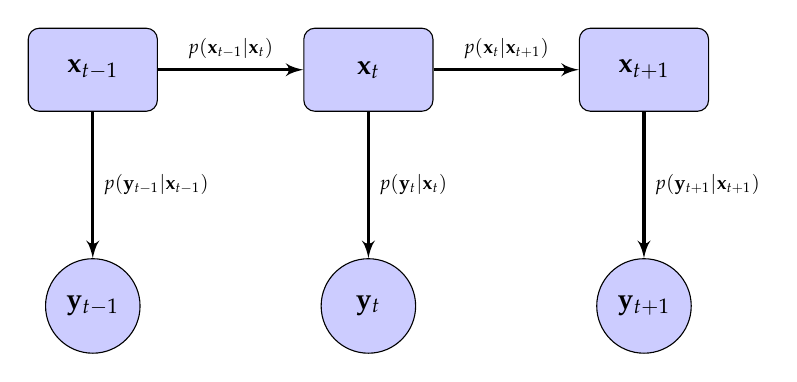
\begin{tikzpicture}[node distance=3.5cm, auto]
        \tikzset{decision/.style={diamond, draw, fill=blue!20, text badly centered,  node distance=2.5cm, inner sep=0pt,align=center}}
        \tikzstyle{block} = [rectangle, draw, fill=blue!20, 
        text width=4em, text centered, rounded corners, minimum height=3em]
        \tikzset{line/.style={draw, very thick, color=black!100, -latex'}}
        \tikzset{circle/.style={shape=circle,draw,minimum size=1.2cm,fill=blue!20,text centered, align=center}}
        \tikzset{decision answer/.style={near start,color=black}}
        
        \node [block] (x1){$\v x_{t-1}$};
        \node [block, right of=x1] (x2) {$\v x_{t}$};
        \node [block, right of=x2] (x3) {$\v x_{t+1}$};
        \node [circle, below of=x1, node distance = 3cm ] (y1){$\v y_{t-1}$};
        \node [circle, below of=x2, node distance = 3cm] (y2) {$\v y_{t}$};
        \node [circle, below of=x3, node distance = 3cm] (y3) {$\v y_{t+1}$};
        
        \path [line] (x1) -- node {\scriptsize $p(\v x_{t-1} | \v x_t)$}(x2);
        \path [line] (x2)-- node {\scriptsize $p(\v x_{t} | \v x_{t+1})$} (x3);
        
        
        \path [line] (x1)-- node {\scriptsize $p(\v y_{t-1} | \v x_{t-1})$} (y1);
        \path [line] (x2)-- node {\scriptsize $p(\v y_t | \v x_t)$} (y2);
        \path [line] (x3)-- node {\scriptsize $p(\v y_{t+1} | \v x_{t+1})$} (y3);
    \end{tikzpicture}
    \caption{Esquematización de un modelo de Markov escondido} \label{dia:hmm}
\end{figure}

\subsection{Predicción, filtrado y suavizado}

Las técnicas de asimilación de datos buscan hacer inferencia estadística en state-space models, es decir que la distribución de interés es $p(\v x | \v y)$. Sin embargo, dado que tenemos muchas realizaciones en el tiempo para $x$ e $y$, debemos ser más específicos. Habitualmente distinguimos 3 distribuciones objetivo de interés:
\begin{itemize}
    \item La distribución predictiva (también llamada de pronóstico o forecast) $p(\v x_t | \v y_{1:s})$ con $s < t$. Esta es la distribución de un estado ``futuro'' usando datos del ``pasado''
    \item La ditribución filtrante (también llamada análisis) $p(\v x_t | \v y_{1:t})$ que informa sobre el estado actual usando observaciones pasadas y actuales
    \item La distribución suavizante $p(\v x_t | \v y_{1:s})$ con $s > t$ que puede ser interpretada como un reanálisis del estado habiendo colectado observaciones futuras al momento sobre el que se hace inferencia.
\end{itemize}

\subsection{Algoritmo \textit{forward-backward}}

En modelos de Markov escondidos, bajo la suposición de que contamos con un modelo de la distribución inicial del estado $p(\v x_0)$, el modelo de transición $p(\v x_t | \v x_{t-1})$ y el modelo observacional $p(\v y_t | \v x_t)$ se puede deducir un algoritmo para obtener de manera secuencial las distribuciones suavizantes. Además, como un subproducto se obtienen las distribuciones filtrantes y las de pronóstico con un grado de separación temporal. 

Si consideramos una ventana de tiempo $t = 1, ..., T$ el algoritmo primero realiza el forward-pass alternando un paso de predicción, en el que obtiene $p(\v x_t | \v y_{1:t-1})$ con un paso de filtrado (también llamado análisis o update) en el que se incorpora la información de la observación a tiempo $t$ y se obtiene $p(\v x_t | \v y_{1:t})$. 

Para $t = 1, ..., T$:
\begin{itemize}
    \item Predicción: $p(\v x_t | \v y_{1:t-1}) = \int p(\v x_t | \v x_{t-1}) p(\v x_{t-1} | \v y_{1:t-1}) d\v x_{t-1}$\label{eq:forward_pred}
    \item Análisis: $p(\v x_t | \v y_{1:t}) \propto p(\v y_t | \v x_t) p(\v x_t | \v y_{1:t-1})$\label{eq:forward_filt}
\end{itemize}
Para hacer la predicción se integra utilizando el modelo de transición. La interpretación de la fórmula es que se calcula la probabilidad de $\v x_t$ dado $\v x_{t-1}$ considerando todos los valores posibles de $\v x_{t-1}$ que obedecen a la distribución filtrante del tiempo anterior. De esta manera, el paso de predicción es el encargado de propagar hacia adelante la distribución del estado. Por otro lado, para hacer el análisis se usa la regla de Bayes y se incorpora $\v y_t$ utilizando el modelo observacional, es decir se actualiza la distribución obtenida en el paso de predicción. Notemos que usamos la convención notacional $\v y_{1:0} = \emptyset$ lo que le da consistencia a las fórmulas ene caso borde de $t = 0$.

Las distribuciones obtenidas en el forward-pass pueden ser utilizadas a su vez para computar las distribuciones suavizantes iterando esta vez hacia atrás, desde el último tiempo hacia el primero de la siguiente manera:

Para $t = T-1, ..., 0$
\begin{itemize}
    \item Suavizado: $p(\v x_t | \v y_{1:T}) = p(\v x_t |\v y_{1:t}) \int \frac{p(\v x_{t+1} | \v x_t)}
    {p(\v x_{t+1} |\v y_{1:t})}
    p(\v x_{t+1} | \v y_{1:T}) d\v x_{t+1}$
\end{itemize}
donde el caso $t = T$ ya está cubierto pues la distribución filtrante para el último tiempo coincide con la suavizante.

La deducción de las fórmulas para predicción, análisis y suavizado están desarrolladas en mayor detalle en el apéndice \ref{appendix:ffbs}.

A pesar de dar una forma general de resolver el problema que plantea la asimilación de datos, en la práctica su aplicación no es tan directa. La integración sobre el espacio de las variables de estado es en general privativa incluso en espacios de dimensionalidad mediana. Por otro lado, hemos hecho la suposición de que contamos con la probabildad de transición $p(\v x_t | \v x_{t-1})$ y esto usualmente no es el caso. El modelo de transición $\mathcal{M}_t$ suele funcionar como una caja negra, de manera que contamos con una forma de muestrear $p(\v x_t | \v x_{t-1})$ pero no necesariamente de evaluar la función de densidad de probabilidad para calcular las integrales necesarias. Existe una gran diversidad de técnicas de asimilación de datos que abordan este problema de distintas maneras. En las secciones subsiguientes describiremos las más relevantes.

\section{Filtro de Kalman}\label{sec:kf}

El filtro de Kalman trabaja sobre una simplificación del problema dado por las escuaciones \ref{eq:transition} y \ref{eq:observation}. Se asume que el modelo de transición de las variables de estado y el modelo observacional son lineales y que las componentes estocásticas se manifiestan como errores gausianos aditivos insesgados. Esto resulta en la siguiente reformulación de las ecuaciones:
\begin{align}
    \v x_t &= \mathbf{M}_t \v x_{t-1} + \gv\eta_t, \label{eq:kf_forward}\\
    \v y_t &= \mathbf{H}_t \v x_t + \gv\nu_t. \label{eq:kf_observational}
\end{align}
donde $\mathbf{M}_t$ y $\mathbf{H}_t$ son operadores lineales y $\gv\eta_t$ y $\gv\nu_t$ son variables aleatorias Gaussianas con media $\v 0$ y matrices de covarianza $\v Q_t$ y $\v R_t$ respectivamente, es decir $\gv\eta_t \sim \mathcal{N}(\v 0, \v Q_t)$ y $\gv\nu_t \sim \mathcal{N}(\v 0, \v R_t)$. Esta configuración del problema asume que tanto el error de modelo como el observacional son insesgados y quedan codificados por completo en las matrices $\v Q_t$ y $\v R_t$.

Si además suponemos que la distribución inicial de $\v x_0$ es Gaussiana, entonces tanto las distribuciones, predictivas y filtrantes serán también Gaussianas. Esto es porque en el paso de predicción, la linealidad del operador de transición preserva la Gaussianidad, lo cual resulta en que en la aplicación de la regla de Bayes en el paso de análisis tengamos verosimilitud y \textit{prior} Gaussianas resultando en una distribución \textit{a posteriori} (la filtrante) también Gaussiana. Este tipo de distribución tiene la propiedad de que puede ser representadas de manera completa a través de dos parámetros: su vector de medias y su matriz de covarianza. Por lo tanto, la tarea del filtro de Kalman es producir secuencias de medias y covarainzas predictivas, $\{\v x_t^f, \v P_t^f\}_{t=1}^{T}$ y medias y covarianzas filtrantes $\{\v x_t^a, \v P_t^a\}_{t=1}^{T}$, de manera que:
\begin{align*}
    p(\v x_t | \v y_{1:t-1}) &\sim \mathcal{N}(\v x_t^f, \v P_t^f) \\
    p(\v x_t | \v y_{1:t}) &\sim \mathcal{N}(\v x_t^a, \v P_t^a)
\end{align*}

Si incorporamos las densidades de probabilidad Gaussianas en las fórmulas de predicción \ref{eq:forward_pred} y análisis \ref{eq:forward_filt} del \textit{forward-pass} se obtienen ecuaciones cerradas para la secuencia de medias y matrices de covarianza de las distribuciones predictivas y filtrantes. Las ecuaciones que se obtienen para el pronóstico son:
\begin{align}
    \v x_t^f &= \mathbf{M}_t \v x_{t-1}^a \label{eq:kf_mean_pred}\\ 
    \v P_t^f &= \v Q_t + \v M_t \v P_{t-1}^a \v M_t^T \label{eq:kf_var_pred}
\end{align}
mientras que para el análisis resulta:
\begin{align}
    \v x_t^a &= \v x_t^f + \mathbf{K}_t (\v y_t - \v H_t \v x_t^f) \label{eq:kf_mean_filter} \\ 
    \v P_t^a &= (\v I - \v K_t \v H_t) \v P_t^f \label{eq:kf_var_filter}
\end{align}
donde $\v K_t = \v P_t^f \v H_t(\v R_t + \v H_t \v P_t^f \v H_t^T)^{-1}$ se denomina matriz de ganancia de Kalman, mientras que el término $(\v y_t - \v H_t \v x_t^f)$ son denominadas innovaciones porque dan cuenta de la diferencia entre el pronóstico y las observación. La deducción de estas fórmulas está desarrollada en el apéndice \ref{appendix:kf}

Notemos que la media de los pronósticos es tan solo la propagación hacia adelante de la media filtrante del tiempo anterior. Por otro lado la matriz de ganancia de Kalman funciona como una matriz de pesos que determina si el estado del análisis será más cercano al pronóstico o si le dará más importancia a la observación. 

\paragraph{Ejemplo unidimensional}
% TODO

\section{3DVar?}

\section{Técnicas por ensambles}
El filtro de Kalman constituye una técnica robusta que da una solución exacta en el caso de modelos lineales con errores Gaussianos aditivos. En ciertos casos es posible considerar linealizaciónes de los operadores $\mathcal{M}_t$ y $\mathcal{H}_t$ y aplicar el filtro de Kalman tradicional con estas aproximaciones. Este método se denomina filtro de Kalman extendido y también producirá estimaciones de las medias y covarianzas predictivas y filtrantes. Aún así, estas dos técnicas no dan respuesta a dos situaciones frecuentes en las aplicaciones de asimilación de datos. Por un lado, es factible que el modelo no sea linealizabe, ya sea porque es tratado como una caja negra o porque la aproximación lineal es imprecisa. En estas situaciones, los pronósticos serán no Gaussianos y es necesario utilizar técnicas que permitan representar otro tipo de distribuciones. Por otro lado, en modelos meteorológicos es común que el espacio de las observaciones tenga alta dimensionalidad ($\sim 10^5$) y el de las variables de estado aún más ($\sim 10^7$) por lo que computar y almacenar las matrices de covarianza $\v P_t^f$ y $\v P_t^a$ sea prohibitivo \citep{Katzfuss2016}. Para dar cuenta de estos problemas se pueden usar técnicas basadas en partículas o ensambles. Estos, en lugar de representar las distribuciones objetivo a través de sus parámetros como en el filtro de Kalman y el filtro de Kalman extendido, se busca representarlas a través de muestras, es decir un ensamble de puntos en el espacio de las variables de estado. Cada punto muestral suele ser denominado partícula o miembro de ensamble de acuerdo a la técnica en cuestión. Vamos a introducir aquí dos familias de métodos basados en ensambles: los filtros de partículas y los filtros de Kalman por ensambles (EnKFs). Los filtros de partículas permiten, en principio, la representación de distribuciones con formas arbitrarias por lo que pueden ser utilizados en escenarios no Gaussianos. Por otro lado, los EnKFs son habitualmente utilizados para mapear el problema al espacio que generan los miembros del ensamble, el cual tiene una dimensionalidad en general mucho menor que el de las variables de estado haciendo posible el cómputo. Es importante aclarar que ninguna de estas técnicas provee una solución \textit{off-the-shelf} para problemas de asimilación de datos arbitrarios e incluso cada método trae aparejado otro conjunto de dificultades técnicas (por ejemplo la degeneración de pesos en el filtro de partículas o el colapso del ensamble en EnKFs). Tanto para filtros de partículas como EnKFs existe una amplia gama de variaciones e implementaciones que introducen características particulares o que buscan resolver o mitigar algún problema en particular. Comenzaremos introduciendo los filtros de partículas porque estos dan una noción clara de por qué tiene sentido usar muestras para representar distribuciones para luego seguir con los EnKFs.

\subsection{Monte Carlo secuencial}

Los filtros de partículas son también conocidos como métodos de Monte Carlo secuencial ya que utilizan el esquema secuencial de dos pasos de predicción-análisis descrito por las ecuaciones \ref{eq:forward_pred} y \ref{eq:forward_filt}. De hecho, el enfoque de estos métodos es el de resolver las integrales de estas ecuaciones, no de manera explícita sino utlizando las aproximaciones empíricas de las distribuciones implicadas. Si tenemos una función de densidad de probabilidades $p$ y una conjunto de partículas $\{\v x^{(i)}\}_{i=1}^N$ muestreadas de manera independiente con esta probabilidad, i.e. $\v x^{(i)}\sim p$, entonces la aproximación empírica de $p$ basada en esta muestra es:
\begin{align*}
    p(\v x) \approx \frac{1}{N}\sum_{i=1}^N \delta(\v x^{(i)} - \v x)
\end{align*}
donde $\delta$ es la delta de Dirac que acumula toda la probabilidad en el punto $\v 0$ siendo nula en todo otro punto. Esta aproximación está sustentada en la ley de los grandes números, dado que se pueden aproximar valores esperados en base a la distribución $p$ utilizando la media muestral de las partículas.
\begin{align*}
    \frac{1}{N}\sum_{i=1}^N \v f(x^{(i)}) \xrightarrow{c. s.} \int f(\v x) p(\v x) d \v x
\end{align*}

Existe una generalización de la aproximación de Monte Carlo denominada muestreo de importancia. A pesar de su nombre es un método para aproximar integrales. Cuando no es posible muestrear de $p$ se puede entonces muestrear otra distribución con densidad $q$ que actúe de proxy de $p$. En principio la única condición para $q$ es que su soporte contenga al de $p$. Este método también admite que no se pueda evaluar exactamente $p$ y $q$ sino que sólo podamos evaluar versiones no normalizadas $\tilde{p}$ y $\tilde{q}$ de estas densidades. Entonces, si tenemos un conjunto de partículas $\{\v x^{(i)}\}_{i=1}^N$ tales que $\v x^{(i)}\sim q$, podemos hacer la aproximación dada por las siguientes fórmulas:
\begin{align*}
    \int f(\v x) p(\v x) d \v x &\approx \sum_{i=1}^N w_i f(\v x^{(i)}) \\
    w_i &= \tilde{w}_i / \textstyle\sum_{i=1}^N \tilde{w}_i \\
    \tilde{w}_i &= \tilde{p}(\v x_i) / \tilde{q}(\v x_i)
\end{align*}
donde $w_i$ son denominados pesos de importancia y $\tilde{w}_i$ son sus versiónes no normalizadas. Por su parte, $q$ es denominada la distribución \textit{propuesta}.

Los métodos de Monte Carlo secuencial producen conjuntos de partículas que aproximan a la distribución filtrante. Estas partícuas además pueden ser ponderadas, es decir pueden traer pesos asociados. Concretamente, para cada tiempo $t$ se obtienen $\{\v x_t^{(i)}, w_t^{(i)}\}_{i=1}^{N}$ tal que sea una aproximación empírica de $p(\v x_t | \v y_{1:t})$.

Los filtros de partículas obtienen estas muestras en dos pasos básicos: primero se muestrean partículas de una distribución propuesta $q$ y luego se computan sus pesos. Con una elección adecuada de $q$ las partículas al tiempo $t$ pueden ser obtenidas a partir de las partículas a tiempo $t-1$ y los pesos pueden ser computados como una actualización de los pesos del tiempo anterior. En particular, dada una muestra pesada $\{\v x_{t-1}^{(i)}, w_{t-1}^{(i)}\}_{i=1}^{N}$ correspondiente al tiempo $t-1$, el procedimiento consiste en:
\begin{itemize}
    \item Muestrear partículas:
        \begin{align*}
            \v x_{t}^{(i)} \sim q(\v x_t | \v x_{t-1}^{(i)}, \v y_t)
        \end{align*}
    \item Actualizar pesos: 
        \begin{align*}
            w_{t}^{(i)} \propto w_{t-1}^{(i)} \frac{p(\v y_t | \v x_t^{(i)}) p(\v x_t^{(i)} | \v x_{t-1}^{(i)})}{q(\v x_t^{(i)} | \v x_{t-1}^{(i)}, \v y_t)}
        \end{align*}
\end{itemize}

Esta implementación es habitualmente llamada SIS (\textit{sequential importance sampling}) y en la práctica tiene el problema de que los pesos suelen concentrarse en una sola partícula, es decir uno de los pesos es prácticamente $1$ mientras que el resto es prácticamente $0$. Este efecto se denomina degeneración del filtro y es indeseable pues la representación muestral de la distribución filtrante pierde expresividad. Además de aumentar el número de partículas existen varias estrategias para mitigar este efecto, la más conocida de ellas es el remuestreo. Este método consiste en muestrar con reemplazo las partículas de la ditribución empirica dada por los pesos. Es decir, una vez computados los pesos se obtiene un nuevo conjunto de partículas con pesos uniformes:
\begin{align*}
    \hat{\v x}_t^{(i)} &\sim \sum_{i=1}^N w_i \delta_{\v x^{(i)}} \\
    \hat{w_i} &= 1 / N
\end{align*}

Esto tiene el efecto que las partículas con mayor peso estarán repetidas y las de menos peso serán eliminadas. A pesar de mitigar la degeneración del filtro causa el problema de empobrecimiento de diversidad del que hablaremos más adelante. No es necesario hacer remuestreo de partículas en cada paso de tiempo y un criterio común para decidir si se hace o no es verificar si el número efectivo de partículas $N_{eff}$ está por debajo de un valor umbral $N_T$. El número efectivo de partículas se puede estimar de la siguiente manera \cite{Arulampalam2002}:
\begin{align*}
    N_{eff} \approx \frac{1}{\sum_{i=1}^N (w_i)^2} \dot{=} \widehat{N_{eff}}
\end{align*}
Este filtro de partículas que incorpora remuestreo suele ser denominado SIR (\textit{sequential importance resampling}) y lo expresamos en forma algortítmica en \ref{algo:sir_pf}.


% TODO: Resolver asignación en algoritmos. Usar := y :~ ?
% TODO: Resolver delta Dirac \delta(x-y) o \delta_y(x)
\begin{algorithm}[H]\label{algo:sir_pf}    
    Muestrear partículas iniciales: $\{\v x_0^{(i)}\}_{i=1}^{N_p} \sim p(\v x_0)$
    
    \For{$t=1, ..., T$}{
        Muestrear partículas de la distribución propuesta: \
        
        \hspace{20pt} $\widehat{\v x}_{t}^{(i)} \sim q(\v x_t | \v x_{t-1}^{(i)}, \v y_t)$ \
        
        Actualizar y normalizar pesos: \
        
        \hspace{20pt} $w_{t}^{(i)} \propto w_{t-1}^{(i)} \frac{p(\v y_t | \widehat{\v x}_t^{(i)}) p(\widehat{\v x}_t^{(i)} | \v x_{t-1}^{(i)})}{q(\widehat{\v x}_t^{(i)} | \v x_{t-1}^{(i)}, \v y_t)}$ \

        Aproximar el número efectivo de partículas: \
        
        \hspace{20pt} $\widehat{N_{eff}} = \frac{1}{\sum_{i=1}^{N_p} (w_i)^2}$ \

        \If{$\widehat{N_{eff}} < N_T$} {
            \begin{flalign*}
                \v x_t^{(i)} &\sim \sum_{i=1}^{N_p} w_i \delta_{\widehat{\v x}_t^{(i)}} & \\
                w_{t}^{(i)} &= 1 / N_p &
            \end{flalign*}            
        }
    }
\caption{Filtro de partículas SIR}
\end{algorithm}

Una de las implementaciones más sencillas de este tipo de filtro es el llamado \textit{bootstrap} y consiste en tomar la distribución propuesta como la probabilidad de transición, i.e., $q(\v x_t | \v x_{t-1}, \v y_t) = p(\v x_t | \v x_{t-1})$. Esto significa que el muestreo de partículas es simpemente aplicar el modelo de transición a todas las partículas del tiempo anterior. Además, las implementaciones más comunes del filtro \textit{bootstrap} hacen remuestreo en cada paso de tiempo. Esto significa que los pesos son sólo calculados para hacer remuestreo pero las partículas que representan a la distribución filtrante tienen pesos uniformes y no hay que almacenarlos. Además esto simplifica el cómputo de los pesos a la expresión $w_{t}^{(i)} \propto p(\v y_t | \v x_t^{(i)})$. En \ref{algo:bootstrap_pf} especificamos este método.

\begin{algorithm}[H]\label{algo:bootstrap_pf}
    Muestrear partículas iniciales: $\{\v x_0^{a, (i)}\}_{i=1}^{N_p} \sim p(\v x_0)$
    
    \For{$t=1, ..., T$}{
        Evolucionar partículas: \
        
        \hspace{20pt} $\v x_{t}^{f, (i)} \sim p(\v x_t | \v x_{t-1}^{a, (i)})$  para $i = 1, ..., N_p$ \
        
        Actualizar y normalizar pesos: \
        
        \hspace{20pt} $w^{(i)} \propto p(\v y_t | \v x_t^{f, (i)})$ \
        
        Remuestrear: \
        
        \hspace{20pt} $\v x_t^{a, (i)} \sim \sum_{i=1}^{N_p} w_i \delta_{\v x^{f, (i)}}$
        }
\caption{Filtro de partículas bootstrap}
\end{algorithm}

La elección de la distribución de transición como distribución propuesta en el filtro de partículas \textit{bootstrap} significa que el muestreo de partículas no es más que evolucionar cada partícula del tiempo anterior utilizando el modelo. Las partículas muestradas constituyen entonces un pronóstico. Esta interpretación no es generalizable al filtro SIR general. Para indicar esto en \ref{algo:bootstrap_pf} usamos el supraíndice $f$ (por \textit{forecast}) en las partículas del pronóstico y $a$ en las de análisis. 

El cómputo de los pesos está dado por la verosimilitud observacional por lo que estos cuantifican cuán afín es cada partícula a la observación. Por su parte, la forma de transformar al conjunto de partículas de pronóstico en una muestra filtrante es a través de el remuestreo. El remuestreo, al ser con reemplazo, tiene el efecto de multiplicar las partículas con pesos altos (cercanas a la observación) y eliminar las partículas con pesos bajos (lejanas a la observación). Este mecanismo se suele comparar con la selección natural, sólo sobreviven y se reproducen las partículas ``más aptas''.

Como se anticipó, el remuestreo introduce otro problema: el empobrecimiento de diversidad. Esto se debe a que tendremos muchas réplicas de las partículas con más peso, es decir una muestra que cubre pbremente el espacio muestral. Este efecto es claramente indeseable y para paliarlo es habitual introducir, luego del remuestreo, un paso en el que las partículas se mutan o se mueven de alguna forma para no tener tantas partículas repetidas. El término mutación proviene de la interpretación del fitro de partículas \textit{bootstrap} como un mecanismo de selección del más apto. Esta modificación de las partículas se puede hacer incorporando pasos de MCMC. También es posible mitigar el problema mediante regularización, utilizando \textit{kernel density estimation} sobre las distribuciones empíricas \citep{Sarkka2013, Arulampalam2002, Ruchi2019}.
% TODO: introducir sin mucho detalle filtros de flujo de langevin y VMPF

% TODO: mejorar este párrafo de ventajas y desventajas de PFs en general
El filtro de partículas SIR tiene la ventaja de hacer pocos requisitos sobre el modelo. En el caso particular del filtro \textit{bootstrap} sólo se necesita evaluar la verosimilitud observacional y muestrear de la probabilidad de transición. Obtener muestra de la probabilidad de transición no es otra cosa que evolucionar el modelo, y este requisito por sí solo significa que el modelo puede ser tratado como una caja negra, una característica deseable en muchas situaciones. Como no hay ninguna suposición sobre las distribuciones, estos métodos pueden ser utilizados en escenarios de no-Gaussianidad y no-linealidad. Por otro lado, este tipo de filtros habitualmente necesitan muchas partículas para tener una buena performance y además padecen de los problemas ya mencionados de degeneración del fitro y empobrecimiento de la diversidad. También es común que muchos pesos sean muy pequeños, lo cual puede causar problemas numéricos. Estos problemas se acentúan en espacios de alta dimensionalidad por lo que en estas situaciones es habitual utilizar filtros de Kalman por ensambles, los cuales introducimos en la siguiente sección.

\subsection{EnKF}

Los filtros de Kalman por ensambles utilizan muestras para mantener estimaciones de las distribuciones objetivo pero incorporan las fórmulas del filtro de Kalman tradicional para actualizar las partículas (en el contexto del EnKF las partículas suelen ser llamadas miembros del ensamble pero utilizaremos las terminologías de manera intercambiable). Para esto es necesario suponer linealidad sobre el modelo de transición y observacional y también errores aditivos Gaussianos: es decir que trabaja sobre el modelo definido por \ref{eq:kf_forward} y \ref{eq:kf_observational}. En realidad, la suposición de que el modelo de transición es lineal puede ser algo relajada en la práctica pero discutiremos esto más adelante.

Supongamos que a tiempo $t-1$ contamos con un ensamble $\{ \v x_{t-1}^{a, (i)} \}_{i=1}^{N_p}$ que representa al análisis. Por las suposiciones que hemos hecho esta muestra será Gaussiana y al aplicar el modelo transicional sobre cada uno de estos miembros del ensamble podemos obtener un ensamble $\{ \v x_{t}^{f, (i)} \}_{i=1}^{N_p}$ del pronóstico a tiempo $t$ el cual constutuirá una muestra Gaussiana. La pregunta entonces, es cómo obtener a partir de este ensamble otro que represente al análisis. La idea de el EnKF es aplicar la ecuación de actualización de la media del filtro de Kalman tradicional \ref{eq:kf_mean_filter} para cada partícula del pronóstico. Esta es la esencia de los EnKF pero para aplicar el concepto correctamente debemos hacer algunas salvedades.

Para aplicar la actualización del filtro de Kalman ecesitamos computar $\v K_t$ la cual por su parte necesita de la matriz de covarianzas del pronóstico $\v P_t^f$. Sin embargo, a diferencia del filtro de Kalman, aquí no propagamos las matrices de covarianzas en el tiempo, sólo una muestra de la distribución y por ello no disponemos de una representación exacta de esta. De cualquier manera, es natural aproximar $\v P_t^f$ con la matriz de covarianza muestral del ensamble del pronóstico, $\widehat{\v P}_t^f$ para obtener una aproximación $\widehat{\v K}_t$ de la matriz de ganancia de Kalman.

Por otro lado, hay que notar que estamos utilizando sobre cada partícula la fórmula de actualización de la media de la distribución, y cada partícula está siendo actualizada en base a la misma observación. Es posible demostrar que si hacemos esto, la covarianza del ensamble del análisis va a estar subestimada. La solución a este problema consiste en actualizar cada partícula usando una perturbación de la observación original. Para obtener el miembro del ensamble $\v x_t^{a, (i)}$ utilizaremos la observación modificada $\v y_t^{(i)} = \v y_t + \v v_t^{(i)}$ con $\v v_t{(i)} \sim \mathcal{N}(\v 0, \v R_t)$. El origen de este problema y su solución son planteados en \cite{Burgers1998}. El método resultante es denominado EnKF estocástico o EnKF con observaciones perturbadas y en \ref{algo:enkf_pert_obs} está descrito de manera algorítmica.

\begin{algorithm}[H]\label{algo:enkf_pert_obs}
    Muestrear ensamble inicial: $\{\v x_0^{a, (i)} \}_{i=1}^{N_p} \sim p(\v x_0)$
    
    \For{$t=1, ..., T$}{
        \For{$i=1, ..., N_p$} {
            $\gv\eta^{(i)} \sim \mathcal{N}(\v 0, \v Q_t)$ \

            $\v x_t^{f, (i)} = \mathcal{M}_t (\v x_{t-1}^{a, (i)}) + \gv\eta^{(i)}$ \
        }

        % Computar $\widehat{\v P}_t^f$, la covarianza muestral de $\{ \v x_t^{f, (i)} \}_{i=1}^{N_p}$ \

        $\widehat{\v x}_t^f = \frac{1}{N_p}\sum_{i=1}^{N_p} \v x_t^{f, (i)}$ \

        $\widehat{\v P}_t^f = \frac{1}{N_p-1}\sum_{i=1}^{N_p} (\v x_t^{f, (i)} - \widehat{\v x}_t^{f}) (\v x_t^{f, (i)} - \widehat{\v x}_t^{f})^T$ \

        $\widehat{\v K}_t = \widehat{\v P}_t^f \v H_t(\v R_t + \v H_t \widehat{\v P}_t^f \v H_t^T)^{-1}$ \

        \For{$i=1, ..., N_p$} {
            $ \v v^{(i)} \sim \mathcal{N}(\v 0, \v R_t)$ \

            $ \v y_t^{(i)} = \v y_t + \v v^{(i)} $ \

            $\v x_t^{a, (i)} = \v x_t^{f, (i)} + \widehat{\v K}_t (\v y_t^{(i)} - \v H_t \v x_t^{f, (i)})$ \
        }

    }
\caption{EnKF estocástico}
\end{algorithm}

Notemos que la suposición de que el modelo de transición es lineal es la suposición que permite asumir que evolucionar los miembros del ensamble hacia adelante va a conservar la Gaussianidad de la muestra. Sin embargo, a diferencia del filtro de Kalman tradicional, no precisamos una expresión matricial $\v M_t$ del operador. El modelo se usa solamente para propagar las partículas hacia adelante por lo cual podemos relajar la hipótesis de linealidad y pensar en un operador general $\mathcal{M}_t$ que si es levemente no lineal podrá preservar la Gaussianidad en los pronósticos y que además puede ser tratado como una caja negra. 

El EnKF que presentamos es solamente una implementación sencilla de esta idea pero la realidad es que existe una gran familia de filtros de Kalman por ensambles desarrollados para diferentes tipos de problemas. Entre ellos podemos destacar 
% TODO: mencion y referencias a EnSRF ETKF, etc.

% TODO: ventajas  desventajas de EnKFs

\subsubsection{Inflación y localización}
\subsection{VMPF}
\section{Estado aumentado}

\chapter{Tratamiento de errores} \label{chp:error_treatment}

\section{Error observacional y de modelo} \label{sec:model_obs_error}

Más allá de los desafíos y dificultades de implementación de las técnicas de asimilación de datos discutidas en el capítulo anterior, la performance de éstas depende crucialmente de la especificación del error de modelo y el observacional. Tanto la predicción de las variables de estado en el tiempo como el proceso observacional tienen fuentes de incerteza \citep{Tandeo2020,Dee1995,Dee1999}. De hecho, las metodologías de asimilación de datos hacen uso de nuestro conocimiento sobre estas incertidumbres para ponderar entre la información que brinda el pronóstico producido por el modelo y la observación. Veremos que una representación incorrecta de estos errores, y en particular de la razón entre estos, puede dar lugar a un exceso de confianza en los pronósticos o en las observaciones. Esto puede ocasionar que se degrade la calidad de las estimaciones de las distribuciones filtrantes y potencialmente que el filtro se desicronice de la trayectoria subyacente que se intenta inferir.

Las variables de estado evolucionan en el tiempo mediante la aplicación del modelo $\mathcal{M}_t$, ecuación \ref{eq:transition}, el cual se diseña para representar en forma simplificada la dinámica del proceso subyacente. Por supuesto, estos modelos para sistemas complejos constituyen una representación imperfecta de la realidad que buscan describir. En lo que llamamos error de modelo, no sólo incluímos este error de representatividad sino también los provenientes de aproximaciones para simplificar el cómputo, errores numéricos y posiblemente la incerteza proveniente del desconocimiento de valores exactos de la parametrización de $\mathcal{M}_t$. Llamaremos laxamente $\v Q$ al error de modelo usando la notación en \ref{eq:kf_forward} que corresponde a la habitual hipótesis en que lo consideremos aditivo, Gaussiano e insesgado. En forma estricta $\v Q$ es la covarianza de la distribución de transición, la cual bajo las hipótesis mencionadas, la determina de manera única. Por otro lado, el error observacional comprende al error de representatividad del operador $\mathcal{H}_t$, las imperfecciones en su especificación y las incertezas intrínsecas de los instrumentos de medición. Análogamente al error de modelo usaremos $\v R$ para referirnos al error observacional. También asumimos para este que es aditivo, Gaussiano e insesgado. Tenemos entonces que $\v Q$ y $\v R$ acumulan el error de diversas fuentes de incerteza y que además en ciertos casos, como el conocimiento incompleto sobre los fenómenos que modelamos, no disponemos de una cuantificación de estas incertidumbres.

Para ilustrar la importancia de especificar correctamente $\v Q$ y $\v R$ consideremos que tenemos el modelo del oscilador armónico introducido en \ref{sec:kf}, totalmente observado con error de modelo $\v Q = \sigma_Q^2 \v I$ y error observacional $\v R = \sigma_R^2 \v I$. Con esta configuración generamos una trayectoria real y sus respectivas observaciones. Luego asimilamos estas observaciones con el EnKF para recuperar el estado real, pero para ello utilizaremos distintos valores de $\sigma_Q^2$ y $\sigma_R^2$. Para evaluar la performance del EnKF en cada repetición, consideraremos dos métricas: la raíz del error cuadrático medio (RMSE) y la cobertura. El RMSE nos informa cuan cerca esta la media de la estimación de la trayectoria real. Por otro lado la cobertura indica en que porcentaje la trayectoria real está incluída en las correspondientes bandas de confianza. Consideraremos un nivel de confianza del 95\% por lo que valores mayores a este indican una sobreestimación de la dispersión de la distribución filtrante mientras que valores menores corresponden a una subestimación. En la figura \ref{fig:QR_performance_trajectories} podemos ver las estimaciones del EnKF para distintas configuraciones de $\v Q$ y $\v R$ (los valores reales están indicados con $\v Q_t$ y $\v R_t$) junto con las métricas obtenidas. En el caso en que se utiliza un $\v Q < \v Q_t$ y un $\v R > \v R_t$ se tiene que la trayectoria estimada es suave, porque al subestimar el error de modelo y sobreestimar el observacional se produce el efecto de que el sistema de asimilación considera más precisos a los pronósticos que a las observaciones y por lo tanto las trayectorias prácticamente no son corregidas y se asemejan a las del modelo. Este efecto se puede ver como un subajuste (\textit{underfit}) a las observaciones y resulta en un RMSE alto; el comportamiento del filtro en esta situación en que las trayectorias prácticamente ignoran a las observaciones suele llamarse divergencia del filtro. En el caso contrario, en que $\v Q > \v Q_t$ y $\v R < \v R_t$, se tiene un efecto de sobreajuste (\textit{overfit}) a las observaciones puesto que se está subestimando su error y por lo tanto las estimaciones se acercan demasiado a ellas dando lugar a trayectorias mucho menos suaves. El caso en el que se utilicen errores de modelo y observacional menores a los reales se tiene que el RMSE es pequeño pero evidentemente la dispersión está subestimada. Por otro lado si ambos errores son mayores que los verdaderos se tiene que la dispersión está sobreestimada. El caso en que se usan los errores reales corresponde entonces a una solución de compromiso entre una correcta cobertura y un RMSE no demasiado grande. Podemos ver en los mapas de calor de la figura \ref{fig:QR_heatmap} que es importante la razón entre $\v Q$ y $\v R$: mientras este cociente es similar al cociente real entre $\v Q_t$ y $\v R_t$ se tendrá una estimación aproximadamente buena de la media, es decir bajo RMSE. Sin embargo la subestimación conjunta de ambos errores (manteniendo la razón entre ellos) produce una mala cobertura (subestimación de la dispersión) y lo contrario sucede con la sobreestimación conjunta. También se hace evidente que en la zona de \textit{overfit} (esquina inferior izquierda del panel de la derecha) se produce menos RMSE que la zona de \textit{underfit} (esquina superior derecha). Esto es debido a que cuando hay \textit{overfit} las estimaciiones tienden a interpolar las observaciones y por lo tanto se mantienen relativamente esn sincronía con las trayectorias reales pero en el caso de \textit{underfit} las estimaciones no se ven influenciadas por las obsevaciones y por lo tanto resultan también independientes de las trayectorias reales. Este análisis, desarrollado en mayor profundidad en \cite{Tandeo2020}, pone en evidencia la importancia de la estimación de estas incertezas, en particular de su especificación conjunta, para maximizar la performance de las técnicas de asimilación de datos.

\begin{figure}[h]
    \centering
    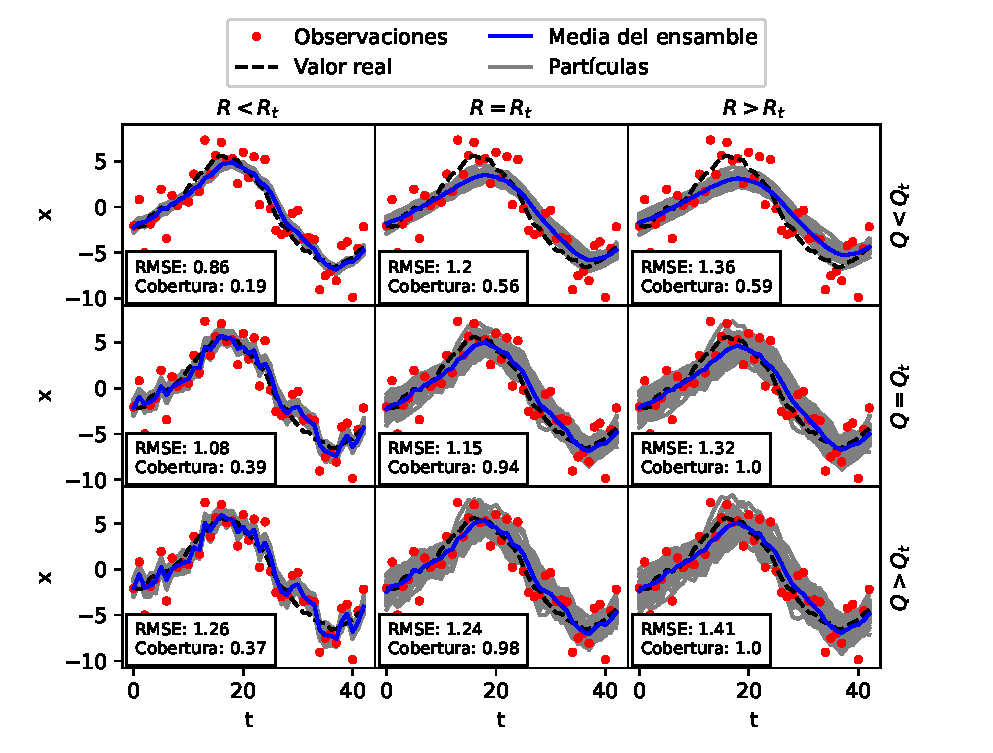
\includegraphics[width=0.75\textwidth]{QR_performance_trajectories.eps}
    \caption{Posición $x$ del oscilador armónico y estimaciones del EnKF para diferentes configuraciones de $\v Q$ y $\v R$.}
    \label{fig:QR_performance_trajectories}
\end{figure}

\begin{figure}[h]
    \centering
    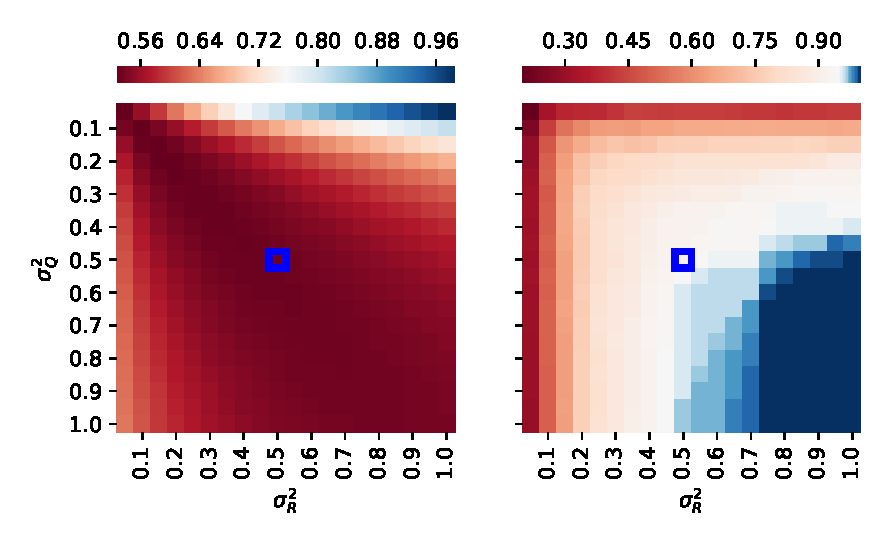
\includegraphics[width=0.75\textwidth]{QR_heatmap.eps}
    \caption{RMSE y cobertura producidas por el EnKF en la estimación del oscilador armónico para para diferentes configuraciones de $\v Q$ y $\v R$. Los valores reales se indican con un recuadro azul. La barra de colores para la cobertura tiene un escalado lineal para que el centro (color blanco) esté en el valor ópimo de cobertura de 95\%.}
    \label{fig:QR_heatmap}
\end{figure}

Como hemos visto en la Sección \ref{sec:enkf}, los métodos basados en ensambles tienen tendencia a colapsar debido a errores de muestreo. El error de modelo cobra una relevancia especial pues está asociada a la dispersión de las partículas del pronóstico y por lo tanto es importante especificarlo correctamente para un buen desempeño del sistema de asimilación. Por su parte, en los filtros de partículas, el error de modelo se relaciona a la incerteza de cada partícula. Muchos filtros de partículas modernos buscan mejorar el muestreo llevando a las partículas a regiones de alta verosimilitud como por ejemplo los filtros de partículas implícitos \citep{Chorin2009, Atkins2013, Zhu2016}, los filtros de flujos de partículas temperados \citep{Daum2009} o el filtro de partículas con mapeo variacional \citep{Pulido2019}. Estos suponen el conocimiento de $\v Q$ y por lo tanto se hace relevante poder acoplarlos con una metodología de estimación de dichos errores.

Se han desarrollado una gran cantidad de métodos para estimar estos errores. En \cite{Stroud2018} se apunta a maximizar la verosimilitud de las innovaciones (la diferencia entre la observación y el pronóstico mapeado al espacio observacional) utilizando inferencia Bayesiana. En otros trabajos se utilizan las covarianzas cruzadas entre innovaciones sucesivas para producir estimaciones de $\v Q$ y $\v R$ (Ver por ejemplo el trabajo seminal de \cite{Mehra1970} y una adaptación moderna basada en esta en \cite{Berry2013}). En el trabajo de \cite{Desroziers2005} se definen estadísticos de diagnóstico basados en las innovaciones que pueden ser utilizados para obtener coeficientes de inflación adaptativos \citep{Li2009}. Notemos que la inflación puede ser vista como un método de estimación del error de modelo puesto que da cuenta de la necesidad de ajustar la incertidumbre de los pronósticos. Sin embargo hay que notar que, por ser multiplicativa, amplificará la covarianza muestral sobretodo en las direcciones en que el pronóstico ya tenga mayor dispersión \citep{Hamill2005}. Otra aproximación al problema, sobre la que nos centraremos aquí, es la maximización de la verosimilitud total a través del algoritmo EM (\textit{expectation-maximization}, \cite{Dempster1977}). Este método fue acoplado con éxito al filtro de Kalman tradicional para estimar $\v Q$ y $\v R$ en \cite{Shumway1982} y con posteridad al filtro de Kalman por ensambles combinado con un suavizador de Kalman por ensambles (ver por ejemplo \cite{Dreano2017}). Un buen compendio de todas estas técnicas se puede encontrar en \cite{Tandeo2020}.

Dentro de toda la variedad de métodos para la estimación de errores observacionales y de modelo distinguimos los métodos \textit{offline} de los \textit{online}. Los primeros toman una ventana de observaciones $\v y_{1:T}$ y dan en base a estas una única estimación para $\v Q$ y $\v R$ para todos los tiempos $t = 1, ..., T$. El algoritmo EM es usualmente implementado de esta manera, utilizando un lote (\textit{batch}) de observaciones (tal es el caso en \cite{Dreano2017, Tandeo2015, Pulido2018}) y aplican el EnKF en combinación con el EnKS. Este procedimiento se adaptó para filtros de partículas en \cite{Lucini2021} sorteando la necesidad de utilizar un suavizador de partículas. En muchas aplicaciones no se utilizan suavizadores porque sólo hay interés en las distribuciones filtrantes y pronósticos y se implementan alternando predicción con análisis. Esto ahorra el costo computacional del suavizado y el almacentamiento de todas las estimaciones anteriores necesarias para el suavizador. En estos escenarios es impráctica o inviable la aplicación de métodos de estimación \textit{offline} y se hace necesario utilizar técnicas \textit{online} (también llamadas secuenciales o adaptativas). Estas producen estimaciones de $\v Q$ y $\v R$ de manera secuencial, es decir en cada ciclo de asimilación y utilizando la información de la observación que está siendo procesada (y no de todo el lote de observaciones de manera simultánea). En el trabajo de \cite{Neal1998} se propone una adaptación \textit{online} para el algoritmo EM y, en el contexto de modelos de Markov escondidos, podemos mencionar el algoritmo propuesto en \cite{Cappe2009} que implementa ideas de EM secuencial acoplados a filtros de partículas y las implementaciones de \cite{Andrieu2003} que utilizan pseudo-verosimilitudes basadas en mini-lotes de datos. También es necesario mencionar que existen implementaciones \textit{online} para estimación de errores que no están basadas en EM como por ejemplo la que se puede encontrar en \cite{Berry2013}.

Para esta tesis, desarrollamos un nuevo método \textit{online} de estimación de error de modelo y observacional basado en EM compatible con filtros de partículas y con EnKFs. La técnica combina las ideas del \textit{batch} EM en la versón de \cite{Dreano2017} con las ideas expuestas por \cite{Cappe2009} y \cite{Andrieu2003} y el resultado está publicado en \cite{Cocucci2021}. Para dar una derivación del método desarrollaremos el algoritmo EM tradicional por lotes en \ref{sec:batchEM} y luego haremos la deducción teórica para adaptar al algoritmo EM a un esquema secuencial en \ref{sec:onlineEM}. Sin embargo, antes de introducir estos métodos haremos la relevante mención de la técnica de estado aumentado. Esta es una metodología muy sencilla de aplicar y que se suele utilizar para la estimación de parámetros ``físicos'' del modelo $\mathcal{M}_t$ y que sin embargo falla para la estimación de errores exponiendo la necesidad de tratar con métodos más involucrados.

\section{Estado aumentado} \label{sec:augmented_state}

En la sección anterior se dicutió la relevancia de utilizar estimaciones apropiadas de los errores involucrados. Los parámetros que codifican a estas incertezas suelen ser llamados parámetros ``estocásticos''. Por otro lado, distinguimos a los parámetros específicos al modelo transicional $\mathcal{M}_t$ los cuales suelen ser llamados parámetros ``determinísticos'' o ``físicos'' ya que usualmente son cantidades interpretables como parte de la dinámica subyacente de las variables de estado $\v x_t$. Es normal que no se cuente con un parametrización precisa del modelo de transición y por lo tanto se requiera de técnicas que permitan estimarlo a partir de mediciones del sistema. En parte, y como fue mencionado en la sección anterior, se puede dar cuenta de la imperfección en la parametrización de $\mathcal{M}_t$ a través del error de modelo y delegar a la estimación de este las incertezas de los parámetros determinísticos. Sin embargo, con la técnica conocida como ``estado aumentado'', es posible estimarlos individualmente y de esta manera calibrar el modelo. Esta consiste en incorporar los parámetros a las variables de estado e interpretarlas como cantidades no observadas del sistema. Si llamamos $\gv\theta_t$ a los parámetros que queremos estimar, construimos entonces el estado aumentado $\tilde{\v x}_t = (\v x_t, \gv \theta_t)$ (notemos la subindexación $t$ que incluímos porque este método admite que los parámetros varíen en el tiempo). Para poder implementar esta idea es necesario extender $\v H_t$ para que interprete a los parámetros como variables no observadas y a $\mathcal{M}_t$ para que actúe sobre estos.

Las técnicas de asimilación de datos pueden inferir sobre variables no observadas ya que la asimilación captura las correlaciones entre estas y las observaciones. En el caso de que esta correlación sea muy débil, el análisis será conservador respecto a la variable no observada que permanecerá cerca del pronóstico. Por lo tanto, este comportamiento se replica para los parámetros en estado aumentado y, en el caso que las correlaciones mencionadas sean los suficientemente fuertes, se podrán obtener estimaciones para los parámetros. Además, como estas estimaciones son secuenciales y siguen la lógica ``pronóstico-análisis'' como el resto de las variables de estado, es posible estimar parámetros con variación temporal dando lugar a un sistema que se auto-calibra \citep{Ruiz2013a}. Sin embargo, hay que mencionar que, como los parámetros son utilizados en el modelo para el paso de tiempo subsiguiente, si los cambios en el parámetro son muy bruscos el sistema tardará en capturarlos, de manera que la adaptividad del método está sujeta a que las variaciones temporales de los parámetros sean lo suficientemente lentas como para que el sistema pueda asimilarlas. 

Para la extensión de $\mathcal{M}_t$ sobre los parámetros es común considerar que actúa como la identidad sobre los parámetros considerando sobre estos una hipótesis de persistencia. Esto significa que si $\gv \theta \in \gv\Theta$ entonces $\mathcal{M}_t |_{\gv\Theta} (\gv \theta) = \gv \theta$. Sin embargo, esto puede causar que las estimaciones se limiten a los valores del prior por lo que es habitual incorporar una caminata aleatoria Gaussiana $\mathcal{M}_t |_{\gv\Theta} (\gv \theta) = \gv \theta + \gv\epsilon_t$ con $\gv\epsilon_t \sim \mathcal{N}(\v 0, \gv\Sigma_{\gv\epsilon})$. Esto contribuye a que el pronóstico de los parámetros consiga una mejor exploración del espacio paramétrico. El valor de $\gv\Sigma_{\gv\epsilon}$ cuantifica la magnitud de los pasos de la caminata aleatoria y se constituye como un hiperparámetro que se puede calibrar para mejorar la performance del sistema de asimilación. El método de estado aumentado también permite modelar una dinámica más compleja para la evolución de los parámetros si esto fuera necesario.

En la figura \ref{fig:augmented_state_example} podemos ver un experimento usando el EnKF en el modelo Lorenz-63 utilizando estado aumentado para estimar $\rho$. Consideramos que el valor verdadero de este parámetro varía en el tiempo de acuerdo a una función sinusoidal. El sistema es capaz de capturar estos cambios y las estimaciones sincronizan con el valor real del parámetro luego de unas pocas iteraciones. La varianza inicial del ensamble se eligió relativamente grande para una mejor exploración del espacio paramétrico.

\begin{figure}[h]
    \centering
    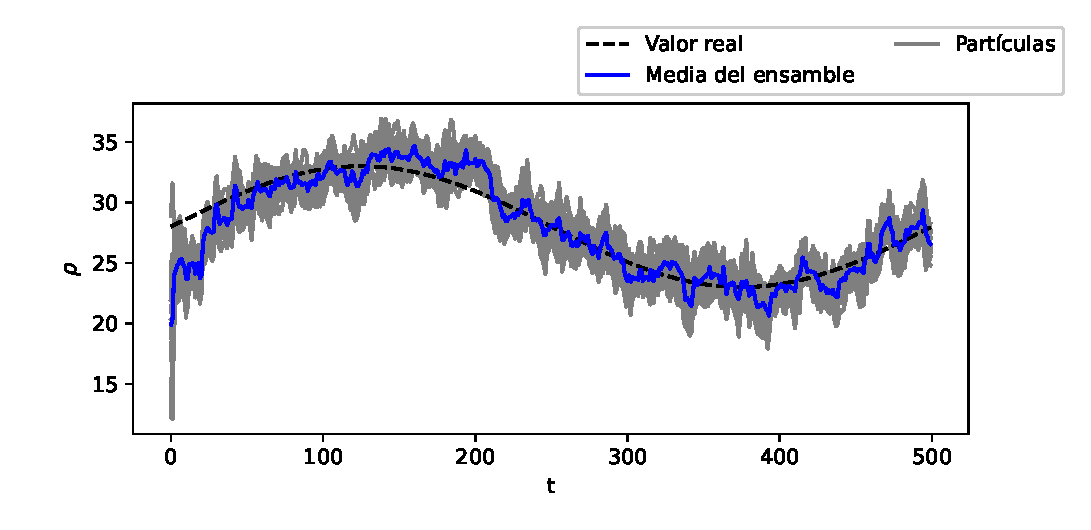
\includegraphics[width=0.75\textwidth]{augmented_state_example.eps}
    \caption{Estimación del parámetro $\rho$ del modelo Lorenz-63 mediante estado aumentado utilizando el EnKF}
    \label{fig:augmented_state_example}
\end{figure}

La técnica de estado aumentado suele ser adecuada para muchos parámetros determinísticos. Sin embargo, no da buenos resultados para la estimación de parámetros estocásticos debido a la falta de correlación entre estos y la información observacional. En \cite{Delsole2010} se puede encontrar una definición algo más precisa de parámetros determinísticos y estocásticos así como una justificación más completa de por qué aumentar el estado con parámetros estocásticos no puede dar buenas estimaciones.

\ma{Quizas se pueda agregar como ejemplo la estimacion del sigma en una caminata aleatoria? Una referencia interesante es: https://doi.org/10.1175/MWR-D-14-00176.1}

\section{Algoritmo EM}

El algoritmo EM se utiliza para obtener estimadores de máxima verosimilitud en sistemas parcialmente observados. Es en realidad una metodología general y no una solución \textit{off-the-shelf}. Su aplicación más conocida es en el contexto de aprendizaje no supervisado para hacer \textit{clustering} modelando el problema con una mezcla de Gaussianas \citep{Bishop2006} pero tiene una gran diversidad de utilidades. Comenzaremos dando su forma general, luego su aplicación en lotes para estimación de matrices de covarianzas en \textit{state space models} con error aditivo Gaussiano y finalmente su adaptación \textit{online}.

El algoritmo EM se aplica en el contexto de un modelo probabilístico en el que contamos con una variable observada $\v y$, variables no observadas $\v x$ y parámetros $\gv\theta$ el cual describe a la probilidad conjunta $p(\v x,  \v y; \gv\theta)$. El objetivo es utilizar datos $\v y$ para estimar el parámetro $\gv\theta$ mediante la maximización de la verosimilitud $p(\v y; \gv\theta)$ o equivalentemente, de su logaritmo. Si dotamos a las variables no observadas de una distribución \textit{a priori} $q(\v x)$ arbitraria podemos obtener la expresión:

\begin{align}
    \log p(\v y; \gv\theta) &=  \log \int p(\v x, \v y; \gv\theta) d\v x \\
    &=  \underbrace{\int q(\v x) \log \frac{q(\v x)}{p(\v x | \v y; \gv\theta)} d\v x}_{KL(\int q(\v x) \rVert p(\v x | \v y; \gv\theta))} + \underbrace{\int q(\v x) \log \frac{p(\v x, \v y; \gv\theta)}{q(\v x)} d\v x}_{\mathcal{L}(q, \gv\theta)} \label{eq:elbo_KL}
\end{align}
\ma{por que se cambia de notacion y se usa mayusculas en lugar d eminusculas para las variables?}
donde $KL$ es la divergencia de Kullback-Leibler y $\mathcal{L}$ es llamada ELBO (\textit{evidence lower bound}). Es común interpretar a $KL$ como una ``distancia'' entre probabilidades y de hecho, cumple que $KL(q \rVert p) \geq 0$ y se anula sí y sólo si $p = q$ en casi todo punto \footnote{Sin embargo notar que la $KL$ no es simetrica por lo que no es un distancia propiamente dicha.}. Al ser $KL$ mayor o igual a 0, esto significa que $\log p(\v y; \gv\theta) \geq \mathcal{L}(q, \gv\theta)$, es decir que la ELBO es una cota inferior de la log-verosimilitud.  

El algoritmo EM provee estimaciones $\gv\theta_0, \gv\theta_1, ...$ tales que $\log p(\v y; \gv\theta_{t+1}) \geq \log p(\v y; \gv\theta_t)$ que convergen a un máximo local de la verosimilitud \citep{Wu1983}. Como dado un $q$ fijo, la $\mathcal{L}(q,\gv\theta)$ es una cota inferior de $\log p(\v y; \gv\theta)$ para todo $\gv\theta$, entonces la idea es maximizar $\mathcal{L}(q,\gv\theta)$ primero respecto a $q$ y luego respecto a $\gv\theta$. Supongamos que ya contamos con la estimación de la $t$-ésima iteración, $\gv\theta_t$. Si queremos obtener $q = \argmax\limits_{q}\mathcal{L}(q,\gv\theta_t)$, notemos que la igualdad \ref{eq:elbo_KL} se satisface para todo $q$ por lo que debemos elegir el valor que anule a la divergencia de Kullback-Leibler, es decir $q = p(\v x | \v y; \gv\theta_t)$. Luego, dejamos fijo $q$ y elegimos $\theta_{t+1} = \argmax\limits_{\gv\theta} \mathcal{L}(q,\gv\theta)$. De esta manera obtendremos que 
\begin{align*}
    \log p(\v y; \gv\theta_t) &= \mathcal{L}(p(\v x | \v y; \gv\theta_t), \gv\theta_t) + \overbrace{KL(p(\v x | \v y; \gv\theta_t) \rVert p(\v x | \v y; \gv\theta_t))}^{0} \\
    &= \mathcal{L}(p(\v x | \v y; \gv\theta_t), \gv\theta_t) \\
    &\leq \mathcal{L}(p(\v x | \v y; \gv\theta_t), \gv\theta_{t+1}) \\
    % &\leq \mathcal{L}(p(\v x | \v y; \gv\theta_t), \gv\theta_{t+1}) + \overbrace{KL(p(\v x | \v y; \gv\theta_t) \rVert p(\v x | \v y; \gv\theta_{t+1}))}^{\geq 0} \\
    &\leq \log p(\v y; \gv\theta_{t+1})
\end{align*}
y por lo tanto que las estimaciones producidas incrementan la verosimilitud.

Notemos además que una vez elegido $q$ tal que anule a la divergencia de Kullback-Liebler en la iteración $t$ obtenemos que:
\begin{align*}
    \mathcal{L}(p(\v x | \v y; \gv\theta_t), \gv\theta) &= \int p(\v x | \v y; \gv\theta_t) \log \frac{p(\v x, \v y; \gv\theta)}{p(\v x | \v y; \gv\theta_t)} d\v x \\
    &= \int p(\v x | \v y; \gv\theta_t) \log p(\v x, \v y; \gv\theta) d\v x - \int p(\v x | \v y; \gv\theta_t) \log p(\v x | \v y; \gv\theta_t) d\v x \\
    &\propto_{\theta} \int p(\v x | \v y; \gv\theta_t) \log p(\v x, \v y; \gv\theta) d\v x \\
    &\dot{=} E_{\gv\theta_t}[\log p(\v x, \v y; \gv\theta)| \v y]
\end{align*}
es decir que la ELBO se puede expresar como una esperanza condicional una vez que elegimos $q$ que maximiza a $\mathcal{L}$. Debido a esto, la maximización sobre $q$ recibe el nombre de \textit{E-step}. Por otra parte el \textit{M-step} corresponde a la maximización sobre $\gv\theta$. El procedimiento admite entonces la caracterización que presentada en el Algoritmo \ref{algo:general_EM} en el que suponemos que se realizan una cantidad prefijada $N_{it}$ de iteraciones, aunque también es posible usar otros criterios de finalización.

\begin{algorithm}[H]\label{algo:general_EM}
    Elegir valor inicial $\gv\theta_0$: \\
    \For{$t=0, 1, ..., N_{it} $}{
        \textit{E-step}: \\
            \hspace{2em}Computar $\mathcal{Q}(\gv\theta, \gv\theta_t) = E_{\gv\theta_t}[\log p(\v x, \v y; \gv\theta)| \v y]$ \\
        
        \textit{M-step}: \\
            $\hspace{2em}\gv\theta_{t+1} = \argmax\limits_{\gv \theta} \mathcal{Q}(\gv\theta, \gv\theta_t)$
    }
\caption{EM general}
\end{algorithm}

La metodología que presentamos tiene la conveniencia de incrementar (o mantener) la verosimilitud en cada paso, sin embargo no garantiza que el máximo encontrado sea un máximo global de la verosimilitud. Cuando la probabilidad conjunta de las variables observadas y no observadas pertenece a la familia exponencial, tenemos simplificaciones importantes en el cómputo y el máximo puede determinarse en forma analítica; esto no siempre es el caso y existen variantes del algoritmo EM que consideran hacer una maximización parcial el \textit{M-step} (EM generalizado). Otra generalización consiste en una optimización parcial en la elección de $q$ en el \textit{E-step} (EM incremental, \cite{Neal1998}) que se implementa mediante la incorporación secuencial de las observaciones. Este método ayuda a una convergencia más rápida del algoritmo, que de otro modo tiene una convergencia en muchos casos lenta. Además, es el punto de partida para las versiones \textit{online} del EM que veremos más adelate.

\paragraph{Ejemplo EM}

Para ilustrar algunas de las características del algoritmo EM consideraremos una varible unidimendional no observada $\v x \sim \mathcal{N}(\gv\theta_t, \sigma_x^2)$ y una observación que responde al modelo $\v y = (\v x + b)^2 + \gv \epsilon$ donde $\gv\epsilon \sim \mathcal{N}(\v 0, \sigma_y^2)$ y $b$ es un escalar. Es decir que tenemos una varible no observada que depende del parámetro verdadero $\gv\theta_t$ y una observación que corresponde a una función cuadrática de la realización de $\v x$ más ruido aditivo Gaussiano. Esto resulta en una log-verosimilitud bimodal como se representa en la figura \ref{fig:EM_example}. También se pueden ver las curvas de la ELBO para dos iteraciones del EM: éstas son cotas inferiores de la log-verosimilitud y en un punto ($\gv\theta = \gv\theta_i$) son iguales. La figura muestra que cada iteración necesariamente tendrá una verosimilitud mayor o igual a las anteriores. Por otro lado quedan en evidencia dos de las debilidades del método: por un lado la convergencia puede ser lenta  puesto que la maximización de la ELBO puede resultar en incrementos pequeños de la verosimilitud, y por otro lado, dependiendo de la estimación inicial $\gv\theta_0$, el algoritmo puede converger a un máximo local. En este ejemplo la convergencia es hacia el menor de los dos máximos, pero si la estimación inicial fuera menor al valor mínimo del valle entre estos el algoritmo convergería al estimador de máxima verosimilitud. Finalmente, notemos que la diferencia entre el máximo de la ELBO para la estimación $\gv\theta_i$ y el valor de la verosimilitud en ese punto es $KL(p(\v x | \v y; \gv\theta_{i-1}) \rVert p(\v x | \v y; \gv\theta_{i}))$ debido a la descomposición de la verosimilitud expresada en la ecuación \ref{eq:elbo_KL}.

\begin{figure}[h]
    \centering
    \includegraphics[width=0.75\textwidth]{EM_example.eps}
    \caption{Log-verosimilitud y ELBO para dos iteraciones del algoritmo EM}
    \label{fig:EM_example}
\end{figure}

\subsection{Batch EM} \label{sec:batchEM}

Los modelos de Markov escondidos son efectivamente sistemas parcialmente observados que en principio, admiten la aplicación del algoritmo EM. Pero además la estructura Markoviana de dependencia temporal de las variables no observadas junto a la independencia condicional de las observaciones puede ser utilizada para obtener una expresión más sencilla de la ELBO. Haremos ahora la suposición de que contamos con un modelo de Markov escondido en un intervalo de tiempos $t = 0, 1, ..., T$ para los cuales tenemos variables latentes $\v x_{0:T}$ y observaciones $\v y_{1:T}$. Las propiedades mencionadas sobre modelos de Markov escondidos nos permiten factorizar a la probabilidad conjunta (necesaria para computar la ELBO) como:
\begin{align}
    p(\v x_{0:T}, \v y_{1:T} ; \gv\theta) &= p(\v x_0 ; \gv\theta) \prod_{t=1}^T p(\v x_t | \v x_{t-1} ; \gv\theta) p(\v y_t | \v x_t ; \gv\theta) \\
    &= p(\v x_0 ; \gv\theta) \prod_{t=1}^T p(\v x_t, \v y_t | \v x_{t-1} ; \gv\theta) \label{eq:joint_factorization}
\end{align}

Para obtener la ELBO correspondiente a la $i$-ésima iteración del método, se elige a $q$ como la distribución de las variables latentes condicionadas a las observaciones y usando la expresión \ref{eq:joint_factorization} se tiene que:
\begin{align}
    \mathcal{L}(p(\v x_{0:T} | \v y_{1:T} ; \gv\theta_i), \gv\theta) &\propto_{\gv\theta} \sum_{t=1}^T \int p(\v x_{1:T} | \v y_{1:T} ; \gv\theta_i) \log p(\v x_t, \v y_t | \v x_{t-1} ; \gv\theta) d\v x_{1:T} \\
    &= \sum_{t=1}^T E_{\gv\theta_i} [\log p(\v x_t, \v y_t | \v x_{t-1} ; \gv\theta) | \v y_{1:T}]
\end{align}
En esta expresión hemos quitado el término correspondiente a $p(\v x_0 ; \gv\theta)$ bajo la suposición de que no hay parámetros desconocidos en la distribución inicial. Esta suposición no es necesaria y de hecho en \cite{Dreano2017} se opta por estimar su media y varianza como partes del vector de parámetros $\gv\theta$ considerados por el algoritmo EM. Ahora haremos una suposición extra que nos permitirá obtener una forma analítica del gradiente de la ELBO: supondremos que $p(\v x_t, \v y_t | \v x_{t-1} ; \gv\theta)$ pertenece a la familia exponencial. Este supuesto no es extremadamente restrictivo puesto que muchas distribuciones relevantes son de la familia exponencial incluyendo, importantemente, a la Gaussiana. En ese caso tendremos entonces que:
\begin{align*}
    p(\v x_t, \v y_t | \v x_{t-1} ; \gv\theta) = h(\v x_t, \v y_t) \exp(\psi(\gv\theta)\cdot s(\v x_{t-1}, \v x_t, \v y_t) - A(\gv\theta))
\end{align*}
donde $s(\v x_{t-1}, \v x_t, \v y_t)$ es llamado el estadístico suficiente, $\psi(\gv\theta)$ la parametrización natural y $h$ y $A$ son funciones \citep{Wasserman2004}. El gradiente de la ELBO respecto al parámetro se puede computar como:
\begin{align}
    \nabla_{\gv\theta} \mathcal{L}(p(\v x_{0:T} | \v y_{1:T} ; \gv\theta_i), \gv\theta) = \nabla_{\gv\theta} \psi(\gv\theta) \cdot \sum_{t=1}^T E_{\gv\theta_i} [s(\v x_{t-1}, \v x_t, \v y_t) | \v y_{1:T}] - T\nabla_{\gv\theta}A(\gv\theta)
\end{align}
con lo cual anulando el gradiente obtenemos la siguiente ecuación
\begin{align} \label{eq:null_elbo_grad}
    \nabla_{\gv\theta} \psi(\gv\theta) \cdot S_i - \nabla_{\gv\theta}A(\gv\theta) = 0
\end{align}
donde usamos la nomenclatura
\begin{align} \label{eq:S_def}
    S_i = \frac{1}{T}\sum_{t=1}^T E_{\gv\theta_i} [s(\v x_{t-1}, \v x_t, \v y_t) | \v y_{1:T}]
\end{align}
El valor del parámetro que cumpla con \ref{eq:null_elbo_grad} será el que maximice la ELBO y por lo tanto el valor subsiguiente del EM, $\gv\theta_{i+1}$. Más precisamente, el valor que anula el gradiente es un punto crítico pero en este caso está garantizado que es un máximo debido a propiedades del Hessiano en familias exponenciales \citep{Wainwright2008}. Notemos que la cantidad $S_i$ es un promedio sobre toda la ventana temporal $t=1, .., T$ de valores esperados de los estadísticos suficientes condicionados a \textit{todas} las observaciones y computado con la última estimación disponible del parámetro, $\gv\theta_i$. El condicionamiento sobre toda la ventana de observaciones implica que el valor esperado esta siendo computado utilizando las distribuciones suavizantes. El método EM que se obtiene para modelos de Markov escondidos bajo la hipótesis de familia exponencial consiste entonces en un \textit{E-step} en el que computamos $S_i$ (\ref{eq:S_def}) y un \textit{M-step} en el que resolvemos la ecuación que anula el gradiente de la ELBO (\ref{eq:null_elbo_grad}).

\subsubsection*{El caso Gaussiano}
Ahora trataremos el caso en el que el error observacional y de modelo sean aditivos y Gaussianos, es decir que tenemos:
\begin{align}
    p(\v x_t | \v x_{t-1}) &\sim \mathcal{N}(\mathcal{M}_t(\v x_{t-1}), \v Q) \\
    p(\v y_t | \v x_t) &\sim \mathcal{N}(\mathcal{H}_t(\v x_t), \v R)
\end{align}
y buscamos estimar $\gv\theta = (\v Q, \v R)$, las matrices de covarianzas del error de modelo y observacional respectivamente. Notemos que, no estamos considerando que estas matrices cambien en el tiempo, es decir que suponemos que son constantes en toda la ventana temporal. Además, debido a la independencia condicional de las observaciones de los modelos de Markov escondidos, tenemos que $p(\v x_t, \v y_t | \v x_{t-1}) = p(\v x_t | \v x_{t-1}) (\v y_t | \v x_t)$ y como supusimos que $p(\v x_t | \v x_{t-1})$ y $(\v y_t | \v x_t)$ son Gaussianas, esto implica que $p(\v x_t, \v y_t | \v x_{t-1})$ también lo es. Por lo tanto seguimos bajo la suposición de familia exponencial que enunciamos anteriormente. La cantidad $S_i$, en este caso puede ser pensada como una tupla $(S_i^{\v Q}, S_i^{\v R})$ y la podemos computar mediante las siguientes expresiones que corresponden al \textit{E-step}:
\begin{align}
    S_i^{\v Q} &= \frac{1}{T}\sum_{t=1}^T E_{\gv\theta_i}[(\v x_t - \mathcal{M}_t(\v x_{t-1}))(\v x_t - \mathcal{M}_t(\v x_{t-1}))^T | \v y_{1:T}] \label{eq:batchEM_SQ} \\
    S_i^{\v R} &= \frac{1}{T}\sum_{t=1}^T E_{\gv\theta_i}[(\v y_t - \mathcal{H}_t(\v x_t))(\v y_t - \mathcal{H}_t(\v x_t))^T | \v y_{1:T}] \label{eq:batchEM_SR}
\end{align}
Por otro lado, la ecuación \ref{eq:null_elbo_grad}, para el caso Gaussiano tiene como solución exactamente a la cantidad $S_i$, con lo cual el \textit{M-step} no requiere ningún cómputo adicional. La verificación de que $\gv\theta = S_i$ anula al gradiente de la ELBO se puede encontar en el apéndice (\ref{appendix:null_grad_elbo}) junto con la representación de una densidad Gaussiana multivariada como miembro de la familia exponencial (\ref{appendix:exp_family}).

Las ecuaciones \ref{eq:batchEM_SQ} y \ref{eq:batchEM_SR}, nos dan fórmulas para computar sucesivas estimaciones de $\v Q$ y $\v R$ y constituyen las fórmulas principales utilizadas en \cite{Tandeo2015, Dreano2017, Pulido2018}. Sin embargo, requieren el cómputo de valores esperados condicionados a la totalidad de la ventana de observaciones, $\v y_{1:T}$. Si se cuenta con una representación de partículas de las distribuciones suavizantes $p(\v x_t | \v x_{1:T})$ para todo $t$, entonces los valores esperados se pueden aproximar con estimadores de Monte Carlo. Notablemente, el EnKS es una técnica que provee estas distribuciones y que también es apropiada para sistemas con errores Gaussianos aditivos; por lo tanto es compatible con esta aplicación del EM. En el algoritmo \ref{algo:em_enks} podemos encontrar la implementación de este método.

\begin{algorithm}[H]\label{algo:em_enks}
    Muestrear ensamble inicial: $\{\v x_0^{a, (i)} \}_{i=1}^{N_p} \sim p(\v x_0)$ \\
    Elegir valor inicial $\gv\theta_0 = (\v Q_0, \v R_0)$:\\
    \For{$i=1, ..., N_{it}$}{
        \textit{E-step}:
        Computar los ensambles de pronóstico, filtrantes usando EnKF con la parametrización $\gv\theta_{i-1}$
            \begin{flalign*}
                \hspace{2em} \{ \v x_t^{f, (j)} \}_{j=1}^{N_p} &\sim p(\v x_t | \v y_{1:t-1}) \hspace{2em} \forall t=1, ..., T && \\
                \hspace{2em} \{ \v x_t^{a, (j)} \}_{j=1}^{N_p} &\sim p(\v x_t | \v y_{1:t}) \hspace{2em} \forall t=1, ..., T &&
            \end{flalign*}
        Utilizar los ensambles de pronóstico y filtrantes para computar los suavizantes mediante EnKS:
            \begin{flalign*}
                \hspace{2em}\{\v x_t^{s, (j)} \}_{j=1}^{N_p} \sim p(\v x_t | \v y_{1:T}) \hspace{2em} \forall t=1, ..., T &&
            \end{flalign*}
            \begin{flalign*}
                \hspace{2em} S_i^{\v Q} &= \frac{1}{T} \sum_{t=1}^{T} \frac{1}{N_p} \sum_{j=1}^{N_p} (\v x_t^{s, (j)} - \mathcal{M}_t(\v x_{t-1}^{s, (j)}))(\v x_t^{s, (j)} - \mathcal{M}_t(\v x_{t-1}^{s, (j)}))^T && \\
                \hspace{2em} S_i^{\v R} &= \frac{1}{T} \sum_{t=1}^{T} \frac{1}{N_p} \sum_{j=1}^{N_p} (\v y_t - \mathcal{H}_t(\v x_t^{s, (j)}))(\v y_t - \mathcal{H}_t(\v x_t^{s, (j)}))^T &&
            \end{flalign*}
        \textit{M-step}: \\
            Asignar nuevos parámetros $\gv\theta_i = (\v Q_i, \v R_i)$
            \begin{flalign*}
                \hspace{2em} \v Q_i &= S_i^{\v Q} && \\
                \hspace{2em} \v R_i &= S_i^{\v R} &&
            \end{flalign*}
    }
\caption{EM-EnKS}
\end{algorithm}

Podemos ver que el algoritmo involucra, para cada iteración, procesar las iteraciones hacia adelante mediante predicción y filtrado con el EnKF, reprocesarlas hacia atrás con el EnKS y luego computar con Monte Carlo las actualizaciones de los parámetros. Las pasadas hacia adelante y hacia atrás provienen de que el EnKF y EnKS son implementaciones del algoritmo \textit{forward-backward}. Esto significa que para utilizar este algoritmo debemos procesar todas las observaciones reiteradas veces. Además del costo computacional, esto implica que las observaciones tienen que ser almacenadas y no se contempla una posible incorporación de nuevas observaciones, situación que sería esperable en un sistema en tiempo real. Aunque el \textit{batch EM} combinado con EnKS es un método robusto para estimar la estrctura general de $\v Q$ y $\v R$ su naturaleza \textit{offline} lo puede hacer impráctico en algunas situaciones y demasiado costoso computacionalmente. Además, no siempre es posible o factible obtener valores esperados respecto a distribuciones suavizantes. Por estos motivos se han desarrollado técnicas \textit{online} o secuenciales de estimación de parámetros estocásticos. 

\paragraph{Ejemplo EM-EnKS} \

Hacemos aquí una aplicación de el EM-EnKS sobre el modelo del oscilador armónico para la estimación conjunta de $\v Q$ y $\v R$. En la figura \ref{fig:em_enks_params} podemos ver el error cuadrático medio entre las estimaciones y el valor real de los parámetros utilizados para generar las observaciones. Además mostramos la media de la diagonal de las matrices estimadas en cada iteración. En realidad cada entrada de las matrices está siendo estimada individualmente (salvo por los elementos simétricos respecto a la diagonal). Notamos que la convergencia es rápida en las primeras iteraciones y luego se desacelera. En la figura \ref{fig:em_enks_rmse_llik} se muestra el error cuadrático medio de las variables de estado suavizadas respecto a los respectivos valores reales y la log-verosimilitud de las observaciones computada mediante la siguiente aproximación dessarrollada en mayor detalle en \ref{appendix:likelihood_montecarlo}:
\begin{align}
    \log p(\v y_{1:T}) \approx \sum_{t=1}^{T} \log \frac{1}{N_p} \sum_{j=1}^{N_p} p(\v y_t | \v x_t^{f, (j)}) \label{eq:likelihood_montecarlo}
\end{align}
Se puede ver que mientras el RMSE disminuye, la verosimilitud aumenta. Notamos también que ambas métricas, son ruidosas debido a que la técnica de asimilación sólo aproxima mediante muestras a las distribuciones.

\begin{figure}[h]
    \centering
    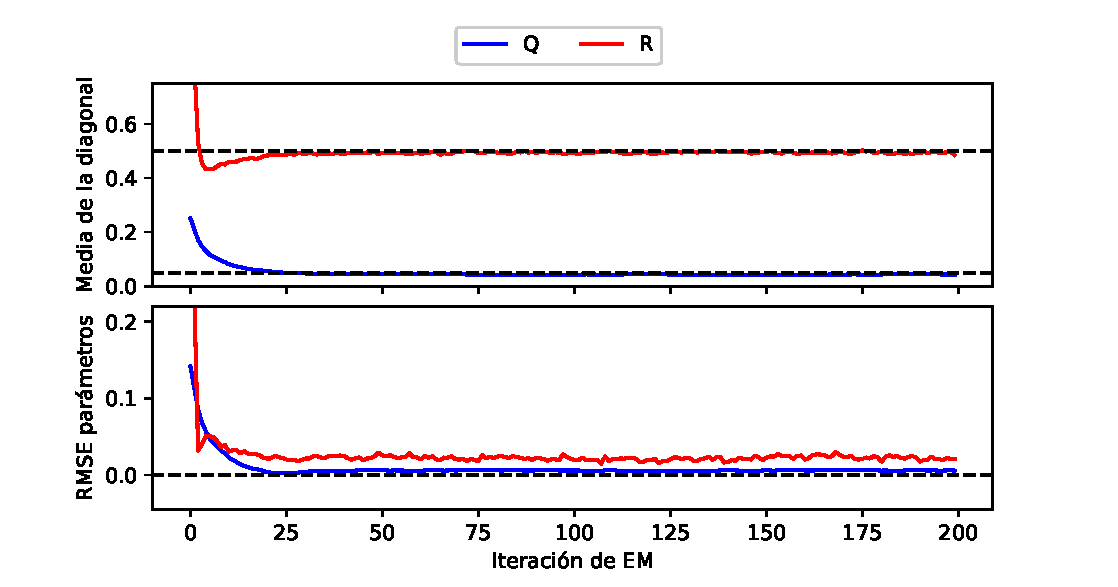
\includegraphics[width=0.75\textwidth]{em_enks_params.eps}
    \caption{Panel superior: estimaciones de las medias de las diagonales de $\v Q$ y $\v R$. Las líneas intermitentes indican los valores reales. Panel inferior: errores cuadráticos medios de las estimaciones respecto a sus valores reales.}
    \label{fig:em_enks_params}
\end{figure}

\begin{figure}[h]
    \centering
    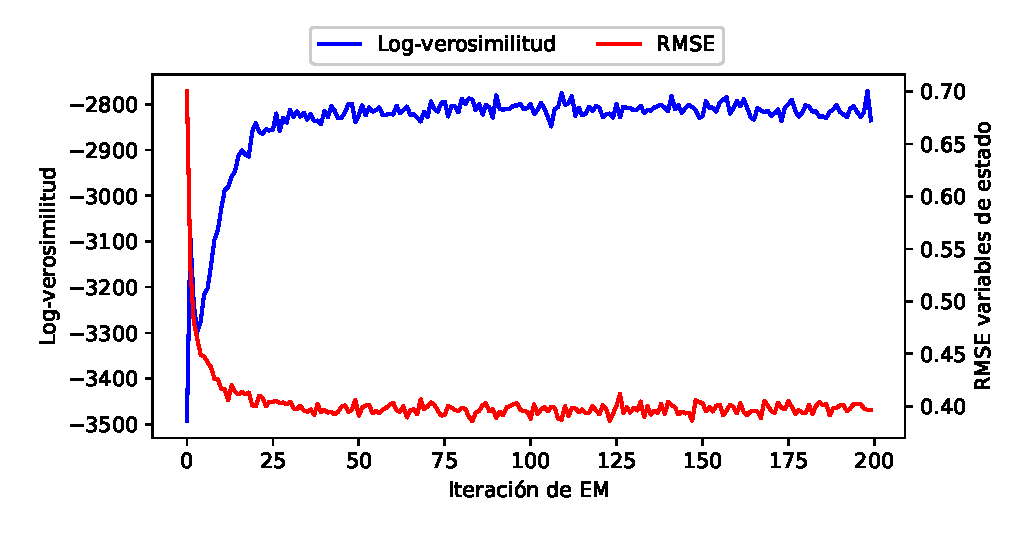
\includegraphics[width=0.75\textwidth]{em_enks_rmse_llik.eps}
    \caption{Log-verosimilitud y RMSE de las variables de estado suavizadas en cada iteración.}
    \label{fig:em_enks_rmse_llik}
\end{figure}

\subsection{EM \textit{online}} \label{sec:onlineEM}

Aquí expondremos el algoritmo \textit{online} basado en EM cuyo desarrollo fue publicado en \cite{Cocucci2021}. El objetivo es obtener una técnica que actualice la estimación del parámetro con cada nueva observación de manera que se puedan descartar las observaciones anteriores que ya han sido procesadas. Si tomamos como punto de partida las ecuaciones \ref{eq:batchEM_SQ} y \ref{eq:batchEM_SR} podemos ver que, cada sumando corresponde a una observación pero que si quisiéramos agregar una observación nueva (correspondiente al tiempo $T+1$) todos estos sumandos deberían ser recomputados. Esto es debido a que los valores esperados están condicionados a toda la ventana observacional anterior, $\v y_{1:T}$. Las nuevas distribuciones predictivas y filtrantes, $p(\v x_{T+1} | \v y_{1:T})$ y $p(\v x_{T+1} | \v y_{1:T+1})$ pueden ser obtenidas o aproximadas utilizando las anteriores distribuciones predictivas y filtrantes que no necesitan ser cambiadas por la incorporación de la nueva observación. Sin embargo, las distribuciones suavizantes $p(\v x_t | \v y_{1:T})$ deben ser cambiadas en cada $t$ por las que tienen en cuenta a la nueva observación, $p(\v x_t | \v x_{1:T+1})$.

En este punto, dado que buscamos procesar observaciones que se hacen disponibles una por una, cambiaremos la notación de las iteraciones del EM y la haremos coincidir con la de las observaciones, puesto que queremos obtener una actualización de los parámetros por cada observación. Entonces consideramos que tenemos observaciones $\v y_{1:T+1}$ y estimaciones de los parámetros $\gv\theta_0, ..., \gv\theta_T$, y buscaremos, a partir de esto, obtener la estimación $\gv\theta_{T+1}$. Más precisamente, buscaremos actualizaciones de la ELBO, es decir que dada una secuencia $S_1, ..., S_T$ buscaremos actualizar $S_T$ para que incorpore la obeservación $\v y_{T+1}$ de manera de obtener $S_{T+1}$. Esto es porque al hacer una extensión \textit{online} de el \textit{E-step} dotamos de esta propiedad a todo el algoritmo, pues el \textit{M-step} seguirá consistiendo en solucionar \ref{eq:null_elbo_grad} para $\gv\theta$ una vez computado $S_{T+1}$. Comenzamos entonces escribiendo la definición de $S_{T+1}$ como en \ref{eq:S_def} con la nueva notación y desglosando la suma de la siguiente manera:
\begin{align}
    S_{T+1} &= \frac{1}{T+1}\sum_{t=1}^{T+1} E_{\gv\theta_T} [s(\v x_{t-1}, \v x_t, \v y_t) | \v y_{1:T+1}] \\
    &= \frac{1}{T+1}\sum_{t=1}^{T+1} \int p(\v x_{t-1}, \v x_t | \v y_{1:T+1}; \gv\theta_T) s(\v x_{t-1}, \v x_t, \v y_t) d\v x_{t-1:t}\\
    &= \frac{1}{T+1} \left( \sum_{t=1}^{T} \int p(\v x_{t-1}, \v x_t | \v y_{1:T+1}; \gv\theta_T) s(\v x_{t-1}, \v x_t, \v y_t)  d\v x_{t-1:t} \right.\\ 
    &\left. + \int p(\v x_{T}, \v x_{T+1} | \v y_{1:T+1}; \gv\theta_T) s(\v x_{T}, \v x_{T+1}, \v y_{T+1}) d\v x_{T:T+1} \right)
\end{align}
Podemos identificar entonces que los primeros $T$ términos de la suma son similares a la cantidad $S_T$ con la salvedad de que en el condicionamiento del valor esperado se incluye la información de la última observación. Haciendo entonces la suposición de que esta última observación no afecta significativiamente a los estados anteriores y sólo influye en el último término se motiva la siguiente aproximación:
\begin{align}
    \widehat{S_{T+1}} &= \left(1 - \frac{1}{T+1}\right) \widehat{S_T} + \frac{1}{T+1} \int p(\v x_{T}, \v x_{T+1} | \v y_{1:T+1}; \gv\theta_T) s(\v x_{T}, \v x_{T+1}, \v y_{T+1}) d\v x_{T:T+1} \\
    &= (1 - \gamma_{T+1}) \widehat{S_T} + \gamma_{T+1} E_{\gv\theta_T} [s(\v x_T, \v x_{T+1}, \v y_{T+1}) | \v y_{1:T+1}] \label{eq:onlineEM_S_rescursion}
\end{align}

Tenemos entonces una fórmula que nos permite computar las aproximaciones $\widehat{S_t}$ para todo $t$ de manera recursiva en base a $S_{t-1}$. Para iniciar la recursión es necesario que contemos con una aproximación inicial $S_0$. Además introducimos $\gamma_t$ que, si bien debe valer $1/t$ para satisfacer \ref{eq:onlineEM_S_rescursion}, puede ser interpretada como una tasa de aprendizaje $\gamma_t \in (0, 1)$, tomando como inspiración técnicas de aproximación estocástica \cite{Legland1997}. Este parámetro va a controlar la ``memoria'' de los estimadores, es decir, pondera la importancia de las estimaciones anteriores respecto al nuevo término que incluye a la última observación. Como veremos luego este parámetro se puede calibrar para obtener comportamientos distintos del método en cuanto a convergencia. Notemos que con este esquema se puede flexibilizar la hipótesis del EM batch de que los parámetros no varían y podemos considerar casos en que los parámetros varíen lentamente en el tiempo. El método resultante tiene algunas similitudes con el propuesto en \cite{Cappe2009} en el que se utiliza una función auxiliar, relacionada a una forma recusiva de suavizado, que permite mantener actualizaciones de $S_t$. Podemos ver que, a pesar de evitar un suavizado hacia atrás hasta la primera observación, el cómputo del valor esperado en \ref{eq:onlineEM_S_rescursion} implica un suavizado de un paso hacia atrás porque el estadístico $s$ depende de $\v x_T$ y el condicionamiento incluye a $\v y_{T+1}$. 

En el algoritmo \ref{algo:onlineEM} se esquematiza el procedimiento de manera general. Notemos que no consideramos una ventana finita de observaciones porque potencialmente se puede seguir iterando a medida que nuevos datos se hacen disponibles. Por otro lado, no hacemos suposiciones sobre los valores iniciales pero sería natural tomar $S_0$ y $\gv\theta_0$ tales que satisfagan \ref{eq:null_elbo_grad}.

\begin{algorithm}[H]\label{algo:onlineEM}
    Elegir valor inicial para el parámetro, $\gv\theta_0$ y el estadístico, $\widehat{S_0}$: \\
    \For{$t = 1, 2, ...$}{
        \textit{E-step}: \\
        $\hspace{2em}\widehat{S_{t}} = (1 - \gamma_{t}) \widehat{S_{t-1}} + \gamma_{t} E_{\gv\theta_{t-1}} [s(\v x_{t-1}, \v x_t, \v y_t) | \v y_{1:t}] $ \\
        \textit{M-step}: \\
        Definir $\gv\theta_t$ como el valor de $\gv\theta$ que solucione: \\
        $\hspace{2em}\nabla_{\gv\theta} \psi(\gv\theta) \cdot \widehat{S_t} - \nabla_{\gv\theta}A(\gv\theta) = 0$ 
        }
        \caption{EM \textit{online}}
\end{algorithm}

De acuerdo a como se compute o aproxime el valor esperado
\begin{align}
    E_{\gv\theta_{t-1}} [s(\v x_{t-1}, \v x_t, \v y_t) | \v y_{1:t}] = \int p(\v x_{t-1}, \v x_t| \v y_{1:t} ; \gv\theta_{t-1}) s(\v x_{t-1}, \v x_t, \v y_t) d\v x_{t-1:t} \label{eq:onlineEM_expected}
\end{align}
tendremos distintas implementaciones del método. En particular daremos dos posibles formas de aproximar esta integral con Monte Carlo. El primero de los métodos está basado en muestreo de importancia y está pensado para ser acoplado a filtros de partículas. La elección de la distribución de importancia evita hacer un paso de suavizado explícito. El segundo se basa en EnKF y agrega un paso hacia atrás de suavizado de manera explícita usando EnKS. 

\subsubsection*{EM \textit{online} con muestreo de importancia} \label{sec:onlineEM_IS}

Para elegir una distribución de importancia conveniente para aproximar \ref{eq:onlineEM_expected} primero desarrollaremos $p(\v x_{t-1}, \v x_t| \v y_{1:t}; \gv\theta_{t-1})$ de la siguiente manera, quitando la dependencia de $\gv\theta_{t-1}$ para mayor claridad:
\begin{align}
    p(\v x_{t-1}, \v x_t| \v y_{1:t}) &= p(\v x_t | \v x_{t-1}) p(\v x_{t-1} | \v y_{1:t-1}) \frac{p(\v y_t | \v x_t)}{p(\v y_t | \v y_{1:t-1})} \label{eq:IS_factorization}
\end{align}
En la factorización (desarrollada con mayor detalle en el apéndice \ref{appendix:IS_factorization}) podemos reconocer al modelo de transición y observacional, a la probabilidad filtrante a tiempo $t-1$ y a la cantidad $p(\v y_t | \v y_{1:t-1})$ que suele ser llamada verosimilitud marginalizada y que no depende de las variables de integración $\v x_{t-1}$ y $\v x_t$. Para aproximar entonces \ref{eq:onlineEM_expected} con muestreo de importancia debemos tener muestras de ambas variables de integración. En lugar de muestrear directamente de $p(\v x_{t-1}, \v x_t| \v y_{1:t})$ \ref{eq:IS_factorization} sugiere que podemos muestrear de $p(\v x_t | \v x_{t-1}) p(\v x_{t-1} | \v y_{1:t-1})$ y obtener pesos proporcionales a $p(\v y_t | \v x_t)$ y, mientras que nos aseguremos de normalizar los pesos, no debemos preocuparnos por la verosimilitud marginal. Esto es conveniente porque disponemos del modelo observacional, $p(\v y_t | \v x_t)$ para evaluar los pesos. Además, como cualquier técnica de filtrado por ensambles produce muestras de la distribución filtrante ya disponemos de las partículas correspondientes a $\v x_{t-1}$ y para obtener las de $\v x_t$ podemos utilizar el modelo de transición.

Si estamos utilizando un método por ensambles de $N_p$ partículas, podemos utilizar nuestra muestra de la distribución filtrante,
\begin{align*}
    \{ \v x_{t-1}^{a, (j)}\}_{j=1}^{N_p} \sim p(\v x_{t-1} | \v y_{1:t-1} ; \gv\theta_{t-1})
\end{align*}
y en base a cada partícula de esta muestra obtener otra, cuyo tamaño denominamos $M_p$, correspondiente a $\v x_t$:
\begin{align*}
    \{ \v x_{t}^{f, (j,l)}\}_{l=1}^{M_p} \sim p(\v x_t | \v x_{t-1}^{a, (j)} ; \gv\theta_{t-1})
\end{align*}
Estas últimas $N_p M_p$ partículas llevan el superíndice $f$ pues se obtienen de la misma manera en que se obtendría un pronóstico (\textit{forecast}) pero haciendo la salvedad de que tenemos $M_p$ partículas por cada punto del tiempo anterior. Con estas muestras podemos ya calcular los pesos no normalizados,
\begin{align*}
    \overline{w_{j,l}} = p(\v y_t | \v x_t^{(j,l)})
\end{align*}
y una vez que obtenemos las versiones normalizadas, $w_{j,l}$ podemos hacer la aproximación de Monte Carlo de la integral:
\begin{align*}
    E_{\gv\theta_{t-1}} [s(\v x_{t-1}, \v x_t, \v y_t) | \v y_{1:t}] \approx \sum_{j=1}^{N_p} \sum_{l=1}^{M_p} w_{j, l} s(\v x_{t-1}^{a, (j)}, \v x_{t}^{f, (j,l)}, \v y_t)
\end{align*}

Este método puede ser implementado con cualquier técnica de asimilación de datos por ensambles ya que solo necesitamos: una representación de partículas filtrante, evaluar el modelo observacional ($p(\v y_t | \v x_t)$) y muestrear del modelo de transición ($p(\v x_t | \v x_{t-1})$), es decir evolucionar el modelo hacia adelante. Por lo tanto, la metodología es compatible con EnKF y filtros de partículas. Notemos también que  es posible tomar $M_p = 1$ pues esto es equivalente a muestrear $(\v x_{t-1}, \v x_t)$ de manera conjunta de la distribución $p(\v x_t | \v x_{t-1}) p(\v x_{t-1} | \v y_{1:t-1}) = p(\v x_t, \v x_{t-1} | \v y_{1:t-1})$. El algoritmo \ref{algo:onlineEM_IS} especifica el método.

\begin{algorithm}[H]\label{algo:onlineEM_IS}

    Muestrear partículas iniciales: $\{\v x_0^{(j)}\}_{j=1}^{N_p} \sim p(\v x_0)$ \\
    Elegir valor inicial para el parámetro, $\gv\theta_0$ y el estadístico, $\widehat{S_0}$: \\
    \For{$t = 1, 2, ...$}{
    Calcular pesos:\\
    \For{$j=1, ..., N_p$}{
        \For{$l=1, ..., M_p$}{
                $\v x_{t}^{f, (j,l)} \sim p(\v x_{t} | \v x_{t-1}^{a, (j)};\gv\theta_{t-1})$ \\
                $w_{j,l} \propto p(\v y_{t} | \v x_{t}^{f, (j,l)} ; \gv\theta_{t-1})$
        }
    }
    Muestrear partículas filtrantes:\\
    $\hspace{2em}\{\v x_{t}^{a, (j)}\}_{j=1}^{N_p}  \sim p(\v x_{t} | \v y_{1:t};\gv\theta_{t-1})$\\
    Computar $\widehat{S_t}$: \\
    $\hspace{2em}\widehat{S_{t}} = (1 - \gamma_{t}) \widehat{S_{t-1}} + \gamma_{t} \sum_{j=1}^{N_p} \sum_{l=1}^{M_p} w_{j, l} s(\v x_{t-1}^{a, (j)}, \v x_{t}^{f, (j,l)}, \v y_t) $ \\
    Definir $\gv\theta_t$ como el valor de $\gv\theta$ que solucione: \\
    $\hspace{2em}\nabla_{\gv\theta} \psi(\gv\theta) \cdot \widehat{S_t} - \nabla_{\gv\theta}A(\gv\theta) = 0$
    }
\caption{EM \textit{online} con muestreo de importancia}
\end{algorithm}

\subsubsection*{EM \textit{online} con un paso de suavizado} \label{sec:onlineEM_OSS}

Una segunda propuesta para obtener una aproximación de Monte Carlo de \ref{eq:onlineEM_expected} es muestrear directamente de $p(\v x_{t-1}, \v x_t| \v y_{1:t})$ para lo cual es necesario obtener la versión suavizada del estado a tiempo $t-1$. El EnKF puede proveernos las partículas correspondientes a $p(\v x_t | \v y_{t-1})$ mientras que podemos obtener una muestra de $p(\v x_{t-1} | \v y_{1:t})$ mediante el EnKS, presentado en el algoritmo \ref{algo:enks}. Notemos además que no es necesario iterar con el EnKS hasta la primera observación sino que basta con hacer un solo paso hacia atrás pues no estamos interesados en las partículas de tiempos anteriores a $t-1$. De esta manera, muestreamos:
\begin{align*}
    \{\v x_t^{a, (j)}\}_{j=1}^{N_p} &\sim p(\v x_t | \v x_{1:t}) \\
    \{\v x_t^{s, (j)}\}_{j=1}^{N_p} &\sim p(\v x_{t-1} | \v x_{1:t})
\end{align*}
donde las partículas suavizantes pueden ser obtenidas del ensamble de pronóstico y el filtrante utilizando las siguientes expresiones:
\begin{align*}
    \v K_{t-1}^s &= \v S_{t-1}^a ( {\v S_t^f}^T \v S_t^f )^{-1} {\v S_t^f}^T \\
    \v x_{t-1}^{j, (s)} &= \v x_{t-1}^{j, (s)} + \v K_{t-1}^s (\v x_t^{j, (s)} - \v x_t^{j, (f)})
\end{align*}
donde $\v S_t^f$ y $\v S_t^a$ son tal como se las especifica en la sección \ref{sec:enkf}. Notemos que, cuando $\v y_t$ es la última observación disponible, la distribución filtrante coincide con la suavizante a ese tiempo y por lo tanto $\v x_t^{s, (j)} = \v x_t^{a, (j)}$. La aproximación de Monte Carlo resulta entonces en:
\begin{align*}
    E_{\gv\theta_{t-1}} [s(\v x_{t-1}, \v x_t, \v y_t) | \v y_{1:t}] \approx \sum_{j=1}^{N_p} s(\v x_{t-1}^{s, (j)}, \v x_{t}^{a, (j)}, \v y_t)
\end{align*}
y la metodología puede ser entonces expresada en forma algorítmica como se expone en el Algoritmo \ref{algo:onlineEM_OSS}.

\begin{algorithm}[H]\label{algo:onlineEM_OSS}
    
    Muestrear partículas iniciales: $\{\v x_0^{(j)}\}_{j=1}^{N_p} \sim p(\v x_0)$ \\
    Elegir valor inicial para el parámetro, $\gv\theta_0$ y el estadístico, $\widehat{S_0}$: \\
    \For{$t = 1, 2, ...$}{
        Computar partículas filtrantes y suavizantes utilizando EnKF+EnKS:\\
    $\hspace{2em}\{\v x_t^{a, (j)}\}_{j=1}^{N_p} \sim p(\v x_t | \v y_{1:t};\gv\theta_{t-1})$ \\
    $\hspace{2em}\{\v x_{t-1}^{s, (j)}\}_{j=1}^{N_p} \sim p(\v x_{t-1} | \v y_{1:t};\gv\theta_{t-1})$ \\
    Computar $\widehat{S_t}$: \\
    $\hspace{2em}\widehat{S_{t}} = (1 - \gamma_{t}) \widehat{S_{t-1}} + \gamma_{t} \frac{1}{N_p}\sum_{j=1}^{N_p} s(\v x_{t-1}^{s, (j)}, \v x_{t}^{a, (j)}, \v y_t) $ \\
    Definir $\gv\theta_t$ como el valor de $\gv\theta$ que solucione: \\
    $\hspace{2em}\nabla_{\gv\theta} \psi(\gv\theta) \cdot \widehat{S_t} - \nabla_{\gv\theta}A(\gv\theta) = 0$
    }
    \caption{EM \textit{online} con suavizado de un paso}
\end{algorithm}
No especificamos que implementación de EnKF o EnKS utilizamos porque potencialmente podemos elegir la que resulte más conveniente. Al estar basado en el filtro de Kalman por ensambles, se tienen los requerimientos usuales para dicho método, es decir errores aditivos Gaussianos en el modelo de transición y observacional. Si consideramos que en el caso Gaussiano, el estadístico suficiente 
se puede expresar como $s(\v x_{t-1}, \v x_t, \v y_{1:t}) = (s^Q(\v x_{t-1}, \v x_t), s^R(\v y_t, \v x_t))$ donde
\begin{align*}
    s^Q(\v x_{t-1}, \v x_t) &= (\v x_t - \mathcal{M}_t(\v x_{t-1}))(\v x_t - \mathcal{M}_t(\v x_{t-1}))^T \\
    s^R(\v y_t, \v x_t) &= (\v y_t - \mathcal{Y}_t(\v x_t))(\v y_t - \mathcal{H}_t(\v x_t))^T
\end{align*}
podemos ver la similaridad entre este método y el EM-EnKS presentado en el algoritmo \ref{algo:em_enks}. Sin embargo, si aplicaramos  la versión \textit{online} a una ventana de tiempo $t = 1, ..., T$, podemos ver que este realiza aproximadamente la misma cantidad de operaciones en total que una única iteración de la versión \textit{offline}. De hecho, el EM \textit{online} requerirá $T$ pasos temporales de EnKF y $T$ pasos simples (de una sola observación) hacia atrás de EnKS: esto es equivalente al pase completo de EnKF+EnKS en la versión \textit{batch}. Por otro lado, la cantidad de evaluaciones de $s$ en el pase completo de la versión \textit{online} es $N_p T$, lo cual coincide con una única iteración del \textit{offline}. El costo computacional es entonces menor para la versión \textit{online} y de aplicación más directa a sistemas secuenciales.

En la implementación de muestreo de importancia, los ensambles representan muestras de las distribuciones. En esta versión basada en EnKF también pero con la importante salvedad de que las muestras están computadas bajo suposiciones de Gaussianidad. Esto significa que se considera que las distribuciones pueden ser representadas solamente con los dos primeros momentos mientras que los de orden superior son ignorados.

\subsection{EM \textit{online}: evaluación experimental}

Expondremos aquí una evaluación experimental del método en distintos escenarios de interés para aplicaciones en asimilación de datos. La configuración de los experimentos consiste en generar trayectorias reales de las variables de estado, mediante la llamada simulación real o natural, y de estas obtener observaciones sintéticas con parametrizaciones conocidas para $\v Q$ y $\v R$. Luego aplicaremos el EM \textit{online} para estimar las variables de estado e importantemente la parametrización original. Sólo utilizamos como fuente de informacion las observaciones sintéticas, es decir que el sistema desconoce las covarianzas y la simulación natural. Utilizaremos el Algoritmo \ref{algo:onlineEM_OSS} con el EnKF estocástico (Algoritmo \ref{algo:enkf_pert_obs}) y el paso de suavizado hacia atrás mediante el RTS-EnKS (Algoritmo \ref{algo:enks}) pero realizando un solo paso hacia atrás. Daremos a esta implementación el nombre OSS-EnKF (por \textit{one step smoother}). Por otro lado, para el Algoritmo \ref{algo:onlineEM_IS} utilizaremos dos implementaciones distintas, una con el EnKF estocástico la cual llamaremos IS-EnKF (por \textit{importance sampling}) y otra con el VMPF la cual denominaremos IS-VMPF. Para esta última implementación notamos que la estimación de la matriz de covarianzas del error de modelo $\v Q$ tiene una relevancia adicional pues utilizamos un kernel $K(\v x, \v x') = (\v x - \v x')^T \beta \v Q (\v x - \v x')$, por lo que el ancho de banda del kernel dependerá de las estimaciones de $\v Q$. Para todas las versiones del EM \textit{online} utilizaremos una tasa de aprendizaje $\gamma_t = t^{-\alpha}$ \citep{Legland1997} donde el valor por defecto es $\alpha = 0.6$ con la excepción de un experimento en el que evaluaremos la performance para distintos valores de $\alpha$. En base a los resultados de dicho experimento es que tomamos el valor por defecto $\alpha = 0.6$.

\subsubsection{Consistencia respecto a valores iniciales}
En este experimento utilizamos el modelo Lorenz-63 y estimamos $\v Q$ con las 3 implementaciones, considerando a $\v R$ conocido. Esto se repite para distintas semillas de los generadores aleatorios y distintos valores iniciales del parámetro. El objetivo es evaluar la consistencia de las estimaciones y la comparabilidad de los métodos. La matriz $\v Q$ utilizada en en la simulación natural es un múltiplo de la identidad. En la figura \ref{fig:lor63_seeds} se muestran las estimaciones de la media de la diagonal de $\v Q$, es decir la varianza media del error de modelo. Notemos que las trayectorias grises corresponden a repeticiones del experimento y no deben ser confundidas con miembros de ensamble, de hecho el método produce una única estimación por iteración. Sin embargo, las repeticiones nos dan una idea de la incerteza de las estimaciones la cual se estabiliza alrededor de los 500 ciclos. Los tres métodos estiman correctamente el valor real del parámetro aunque los basados en importance sampling muestran una ligera subestimación. La velocidad de convergencia y la variabilidad en las estimaciones es también similar en todos los métodos.
\begin{figure}[h]
    \centering
    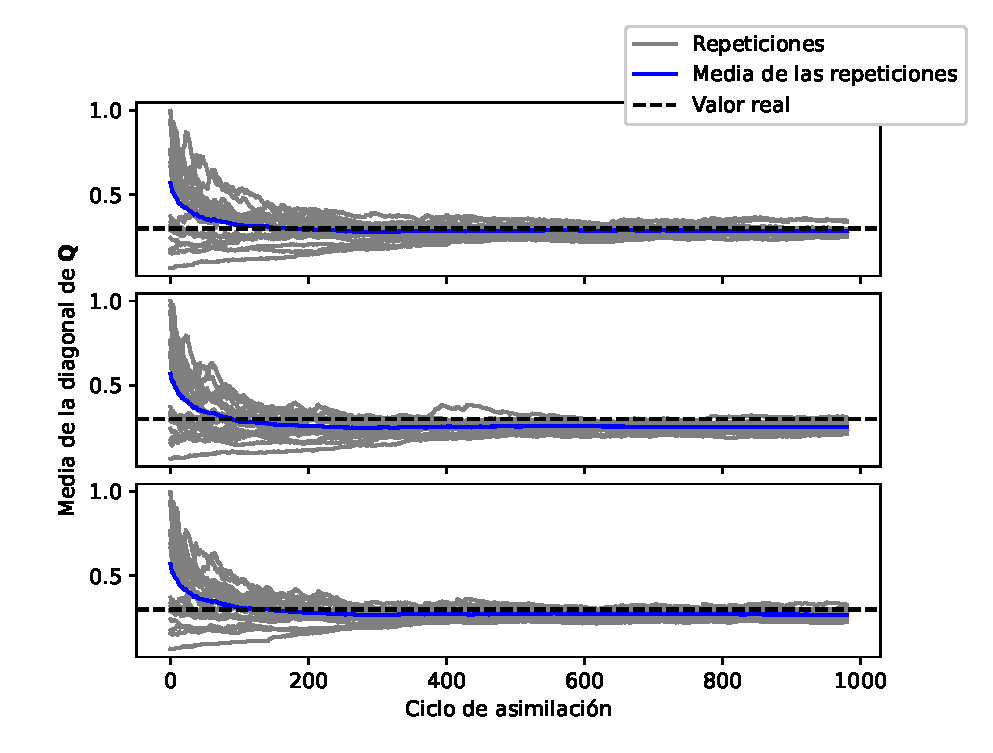
\includegraphics[width=0.75\textwidth]{lor63_seeds.eps}
    \caption{Estimaciones de la media de la diagonal de $\v Q$ con OSS-EnKF (panel superior), IS-EnKF (panel medio) y IS-VMPF (panel inferior).}
    \label{fig:lor63_seeds}
\end{figure}

\subsubsection{Efecto de la tasa de aprendizaje}
Para evaluar el efecto de la tasa de aprendizaje en las estimaciones realizamos un experimento similar al anterior: estimamos una matriz $\v Q$ diagonal considerando $\v R$ conocida en el modelo Lorenz-63. En cada simulación utilizamos el mismo set de observaciones sintéticas pero cambiamos el valor de $\alpha$ de la tasa de aprendizaje. En la figura \ref{fig:lor63_alphas} se muestran las estimaciones para la media de la diagonal de $\v Q$. Para valores mayores de $\alpha$ la convergencia es lenta e incluso puede no lograrse en 10000 ciclos de asimilación. Por otro lado, para valores más pequeños se obtiene una convergencia mucho más rápida. Las estimaciones que produce el método son una ponderación entre la estimación de la iteración anterior con el promedio de los estadísticos suficientes correspondientes a la observación que está siendo procesada. Cuando $\alpha$ es más cercano a 1 se da más peso a la estimación anterior y menos a la información introducida por la última observación. Esto puede interpretarse como que el método tiene más memoria por lo que las nuevas iteraciones no cambian sustancialmente las estimaciones, con lo cual estas resultan menos ruidosas pero la convergencia se realentiza. Por el contrario, para valores menores de $\alpha$ se le da mayor peso a los estadísticos suficientes correspondientes a la última observación y menos a las estimanciones anteriores. Esto acelera la convergencia pero las trayectorias se hacen más ruidosas debido al error de muestreo.
\begin{figure}[h]
    \centering
    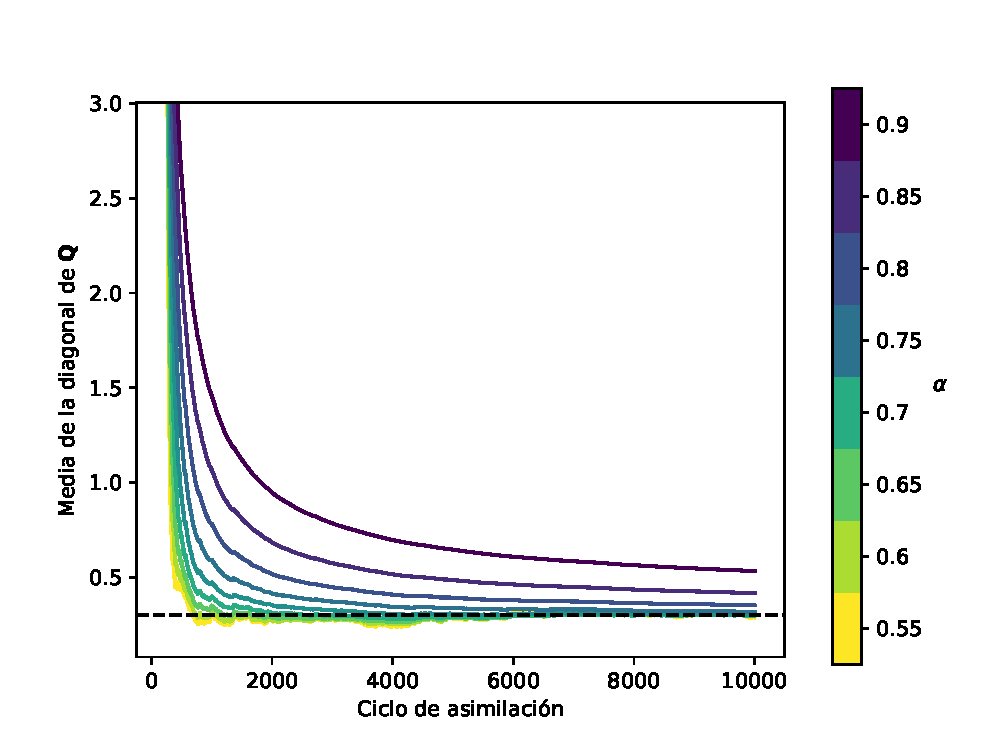
\includegraphics[width=0.75\textwidth]{lor63_alphas.eps}
    \caption{Estimaciones de la media de la diagonal de $\v Q$ con OSS-EnKF (panel superior), IS-EnKF (panel medio) y IS-VMPF (panel inferior).}
    \label{fig:lor63_alphas}
\end{figure}

\subsubsection{Estimación de covarianzas}
En aplicaciones geofísicas es normal que las variables estén correlacionadas espacialmente. En estos sistemas es natural que el error de modelo también reproduzca estas correlaciones. Esto resulta en que la matriz $\v Q$ tenga una estructura con valores no nulos fuera de la diagonal. Para este conjunto de experimentos consideraremos el modelo Lorenz-96 \citep{Lorenz1996}, determinado por las siguientes ecuaciones diferenciales:
\begin{align}
    \frac{d X_n}{d t} = X_{n-1}(X_{n+1} - X_{n-2}) - X_n + F \hspace{1em} \forall n = 1, ..., N_x 
\end{align}
Tomaremos condiciones de frontera periódicas, es decir, $X_{-1} = X_{N_x-1}, X_0 = X_{N_x}, X_1 = X_{N_x+1}$. Este modelo busca emular el comportamiento de una variable atmosférica en un círculo de latitud con un forzado externo representado por $F$. Consideraremos, además de la varianza del error, representado por valores positivos en la diagonal de $\v Q$, covarianzas positivas e uniformes entre variables adyacentes. Esto significa que $\v Q_{i, (i+1)\%N_x} = \sigma_{ady}^2 > 0 \hspace{1em} \forall i = 1, ..., N_x$. Los valores en la diagonal también serán uniformes de manera que $\v Q_{i, i} = \sigma_{diag}^2 > 0 \hspace{1em} \forall i = 1, ..., N_x$. Para estimar esta matriz utilizamos las tres implementaciones del EM \textit{online} y también con 25 iteraciones del EM \textit{offline} en la implementación del Algoritmo \ref{algo:em_enks}. Notemos que la versión \textit{online} es una aproximación del \textit{offline} por lo que la segunda constituye una base de comparación razonable para la primera.

A pesar de que la matriz $\v Q$ tiene una estructura que admite una representación de sólo dos parámetros, las estimaciones producidas por cualquiera de los métodos son entrada por entrada (salvo simetría pues los estadísticos suficientes son simétricos). Para verificar que el comportamiento de las estimaciones en cada entrada es consistente mostramos en la figura \ref{fig:lor96_online_entrywise} las trayectorias correspondientes. Podemos observar que estas se agrupan correctamente alrededor de los valores de la matriz $\v Q$ original.
\begin{figure}[h]
    \centering
    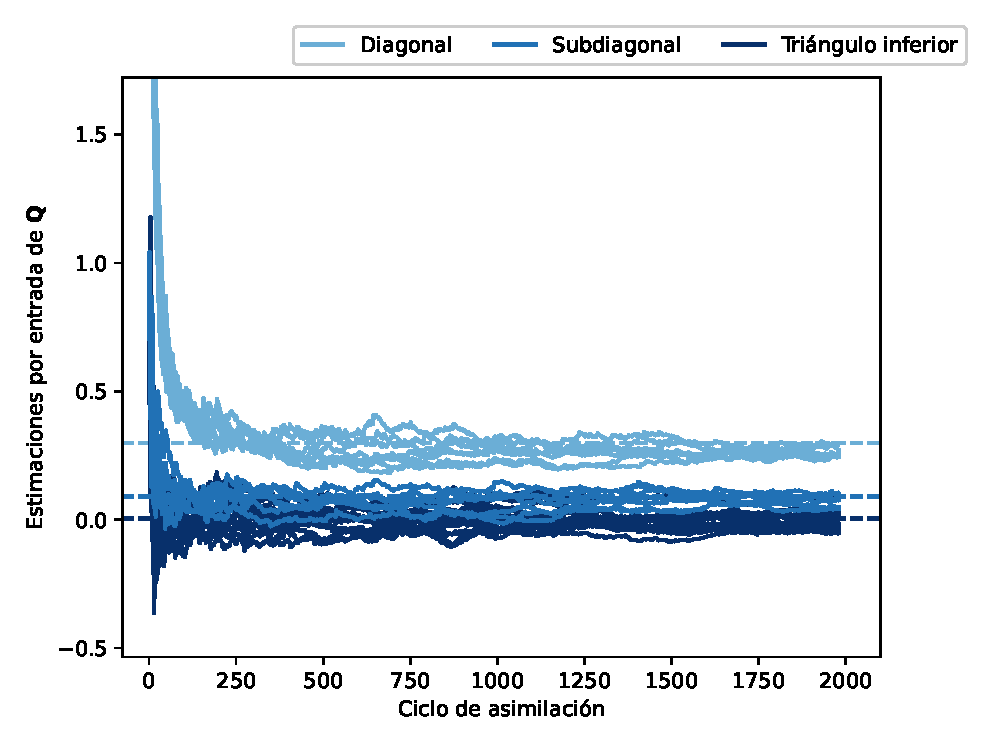
\includegraphics[width=0.75\textwidth]{lor96_online_entrywise.eps}
    \caption{}
    \label{fig:lor96_online_entrywise}
\end{figure}
\begin{figure}[h]
    \centering
    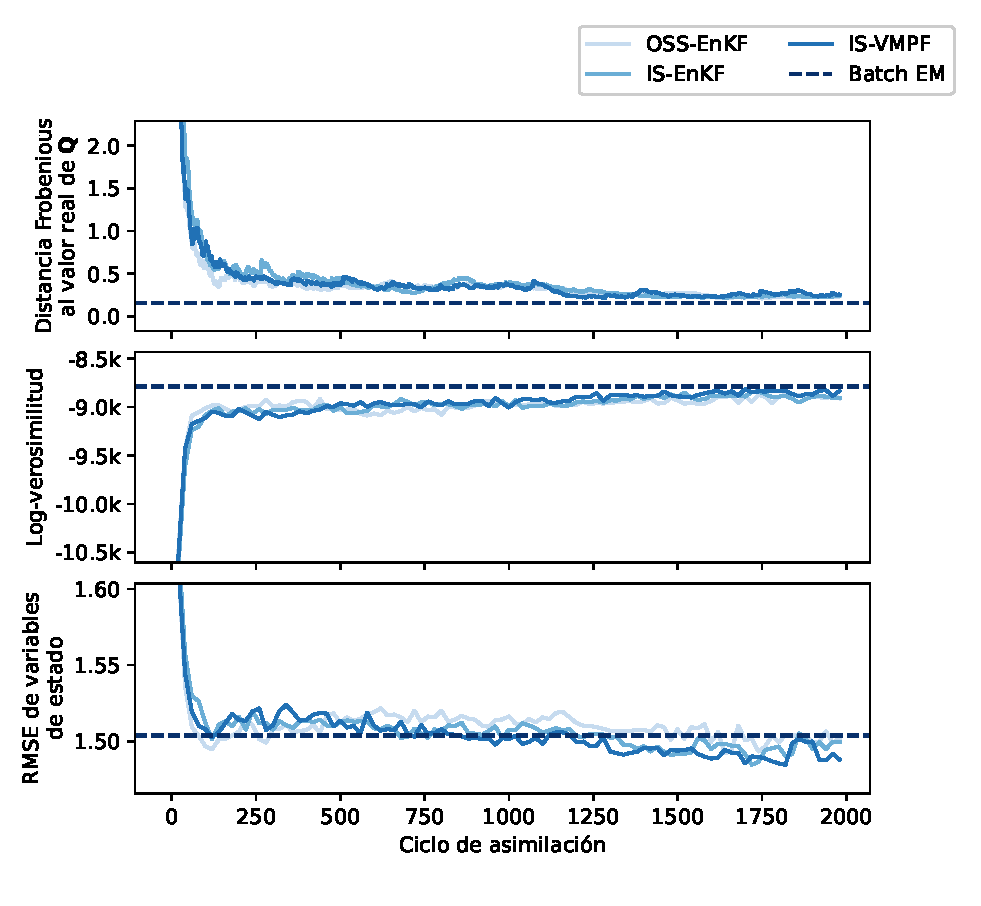
\includegraphics[width=0.75\textwidth]{lor96_online_batch.eps}
    \caption{}
    \label{fig:lor96_online_batch}
\end{figure}
En la figura \ref{fig:lor96_online_batch} se puede ver la distancia Frobenious de las estimaciones de todos los métodos. Los errores de las estimaciones en los métodos secuenciales se aproximan con velocidad similar entre ellos al error obtenido por el EM \textit{offline}. Además, para cada estimación de $\v Q$ se realizó un filtrado con el EnKF con $\v Q$ fijada en el valor de la estimación. Del resultado de estos filtrados computamos el RMSE de las varibles de estado y la log-verosimilitud obtenida. Se puede ver en la figura \ref{fig:lor96_online_batch} que la performance según estas métricas, son similares a las del EM \textit{batch}.

Finalmente, realizamos un experimento similar pero considerando que la matriz $\v Q$ varía lentamente en el tiempo de acuerdo a una función sigmoide. La versión \textit{batch} del EM produce una única estimación del parámetro para toda la ventana observacional. Por el otro lado los métodos secuenciales, al producir una estimación por cada observación son capaces de capturar cambios en el parámetro. Notemos sin embargo que las estimaciones, al tener ``memoria'' no pueden capturar cambios muy abruptos. En la figura \ref{fig:lor96_varyingQ} se observa que todos los métodos responden a los cambios en $\v Q$ aunque, especialmente para los valores en la diagonal se produce una subestimación respecto al valor real. Esto podría deberse a que el efecto de la memoria del método provoque que las estimaciones aún tengan una tendencia hacia los valores más tempranos y más pequeños de la ventana temporal. 
\begin{figure}[h]
    \centering
    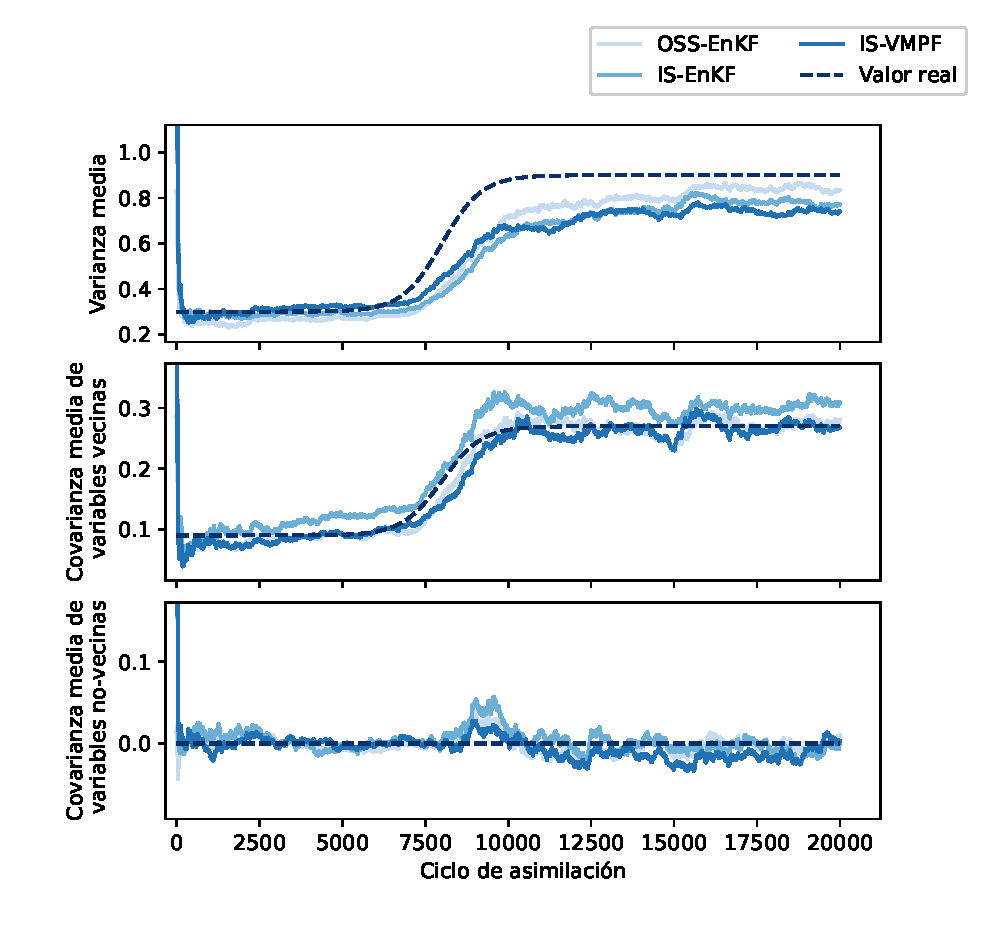
\includegraphics[width=0.75\textwidth]{lor96_varyingQ.eps}
    \caption{}
    \label{fig:lor96_varyingQ}
\end{figure}

\clearpage

\subsubsection{Estimación conjunta de $\v Q$ y $\v R$} \

Hasta ahora nos hemos enfocado en la especificación del error de modelo puesto que es una fuente de incerteza de la cual, en la mayor parte de los casos, no tenemos forma de determinar debido a que suele provenir del desconocimiento del proceso subyacente. El error observacional por otro lado, muchas veces se puede aproximar pues conocemos mejor el proceso observacional. Sin embargo, como hemos visto en la sección \ref{sec:model_obs_error} la especificación de ambas incertezas es importante y de hecho existe interacción entre ambas cantidades. Por esto se hace importante estudiar la estimación conjunta de $\v Q$ y $\v R$. En este experimento lo hacemos tomando a ambas como matrices diagonales múltiplos de la identidad: $\v Q = \sigma_{\v Q}^2$ y $\v R = \sigma_{\v R}^2$. El modelo utilizado es el Lorenz-96 con 8 variables, todas observadas. Consideramos dos escenarios: en el primero tenemos errores observacionales y de modelo similares, $\sigma_{\v Q}^2 = 0.3$ y $\sigma_{\v R}^2 = 0.5$; mientras que en el segundo tomamos un error observacional mayor, $\sigma_{\v R}^2 = 1.5$. El efecto que se encuentra cuando $\v Q$ y $\v R$ son similares es que la verosimilitud tiene un máximo mejor definido. En la figura \ref{fig:lor96_contours} vemos los contornos de la verosimilitud en función de $\sigma_{\v Q}^2$ y $\sigma_{\v R}^2$ para ambos casos. El panel izquierdo corresponde al escenario de errores similares y se puede observar que el máximo es más definido que el escenario con errores disímiles del panel derecho. Además graficamos las trayectorias de las estimaciones para distintos valores iniciales. Se puede ver que cuando el máximo está mejor definido las estimaciones son más precisas. Finalmente notamos que los valores de la verosimilitud son menores en el caso de mayor error observacional, lo cual es esperable porque las observacions son menos precisas.

\begin{figure}[h]
    \centering
    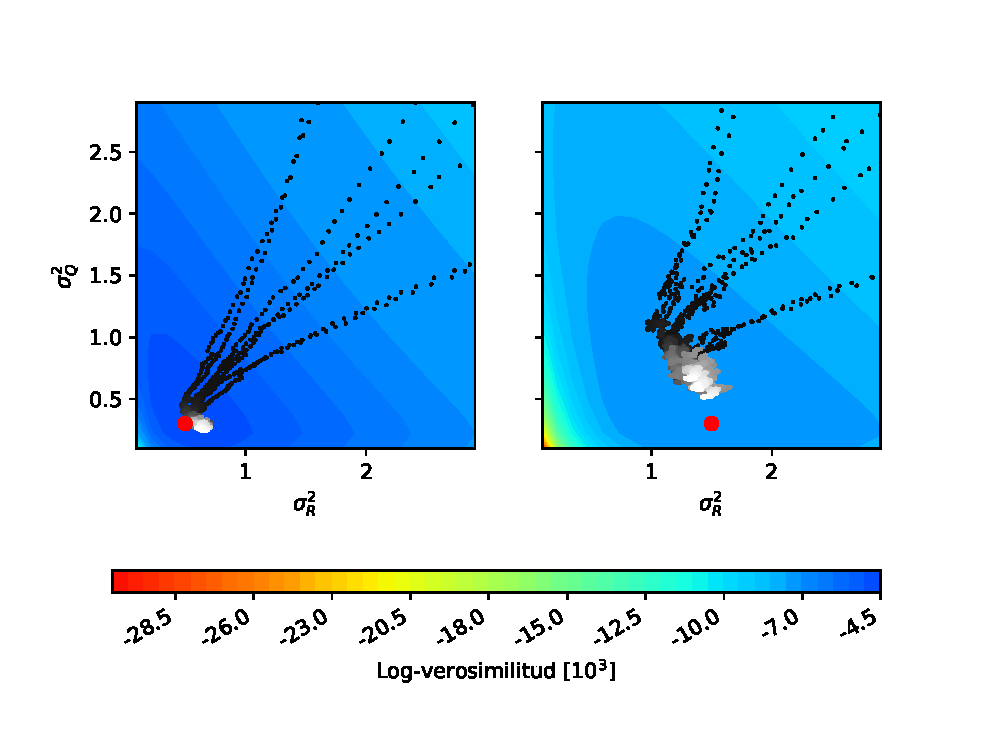
\includegraphics[width=0.75\textwidth]{lor96_contours.eps}
    \caption{}
    \label{fig:lor96_contours}
\end{figure}

\subsection{Discusión}

La metodología de EM \textit{online} que desarrollamos muestra resultados prometedores y da respuesta a algunos de los desafíos que típicamente se presentan en escenarios de asimilación de datos. La técnica permite evitar el uso de suavizadores sobre grandes ventanas temporales lo que la hace computacionalmente menos costosa que las versiones por lotes del EM y especialmente adecuada para contextos de asimilación de datos secuencial. Es importante notar que la performance puede depender de la tasa de aprendizaje utilizada. La técnica permite la estimación de varianzas pero también covarianzas en los errores de las variables de estado y adicionalmente detecta coambios temporales lentos en los parámetros estocásticos. No evaluamos el desempeño del método en espacios de alta dimensionalidad ya que en estos casos las mismas técnicas de asimilación pueden comenzar a tener peor rendimiento debido a que se dificulta la representación de distribuciones mediante muestras en este tipo de espacios.

\chapter{Modelos epidemiológicos}

\section{Modelos compartimentales}

Para modelar la propagación de enfermedades infecciosas, es muy habitual utilizar modelos compartimentales basados en ecuaciones diferenciales. Estos pueden ser utilizados para predecir y comprender situaciones epidemiológicas, ayudar a la toma de decisiones y simular situaciones hipotéticas así como también se pueden utilizar para estimar parámetros. Su origen se remonta a los años 20 del siglo pasado y suele atribuirse a \cite{Kermack1927}. Estos consisten en modelar la población distinguiendo subpoblaciones de acuerdo a categorías epidemiológicas. Por ejemplo, el emblemático modelo SIR, distingue a las subpoblaciones susceptible ($S$), infectada ($I$) y recuperada ($R$). Este se puede expresar mediante el siguiente sistema de ecuaciones diferenciales,
\begin{align}
    \frac{\partial S}{\partial t} &= -\beta \frac{SI}{N}\\
    \frac{\partial I}{\partial t} &= \beta \frac{SI}{N} - \gamma I \\
    \frac{\partial R}{\partial t} &= \gamma I
\end{align}
Estas ecuaciones suponen una población constante de tamaño $N$: notemos que las ecuaciones suman 0 por lo que la población total se mantiene. La velocidad con que los individuos susceptibles se infectan es proporcional a la cantidad total de susceptibles, $S$ y a la proporción de infectados de la población $\frac{I}{N}$. La constante de proporcionalidad $\beta$ es llamada la tasa de infección y cuantifica la transmisibilidad de la enfermedad. Por su parte, la velocidad con que los infectados se recuperan es proporcional a la cantidad de infectados y la constante de proporcionalidad $\gamma$ es llamada tasa de recuperación.

El modelo SIR, aunque sencillo, merece mención pues tiene los elementos básicos con los que se puede construir un modelo compartimental. Como vimos, la entrada y salida de cada compartimento se describe con una ecuación diferencial y con esta idea se pueden diseñar distintas estructuras de subpoblaciones para describir las situaciones que se deseen modelar. Es común ver en este tipo de modelos la subpoblación de los decesos $D$ que permite distinguir a la porción de la población que muere a causa de la enfermedad, o la subpoblación de los expuestos $E$ se suele ver en modelos para enfermedades virales en que las personas se infectan e incuban el virus sin ser infecciosas antes de pasar al compartimento $I$. De esta manera tenemos modelos como el SEIRD que considera estas subpoblaciones, o el SIS que no tiene en cuenta una categoría de recuperados que no contagia sino que las personas, al curarse de la enfermedad vuelven a ser susceptibles. Otros modelos como el SIRV, consideran el comprtimento de vacunados $V$ que pasan a ser inmunes al contagio. En, general podemos distinguir 3 tipos distintos de compartimentos: aquellos que actúan de fuente, es decir que solo decrecen o se mantienen, y por lo tanto los términos en las ecuaciones diferenciales son sólo negativos, los compartimentos intermedios, cuyas ecuaciones incluyen términos positivos y negativos y finalmente los compartimentos que actúan de resumidero, es decir que sólo crecen o se mantienen los cuales sólo incluyen términos positivos. Por ejemplo, en el modelo SIR el compartimento $S$ actúa a modo de fuente, $I$ es un compartimento intermedio y $R$ actúa de resumidero. Típicamente las trayectorias de las fuentes tienen una forma sigmoidea decreciente y las de los resumideros son sigmoideas decrecientes mientras que los compartimientos intermedios suelen exhibir un comportamiento con forma de campana. En la figura \ref{fig:sir_example} se puede observar esto en las trayectorias generadas por un modelo SIR.

\begin{figure}[h]
    \centering
    \includegraphics[width=0.75\textwidth]{sir_example.eps}
    \caption{}
    \label{fig:sir_example}
\end{figure}

Los modelos compartimentales pueden además incluir otras características como varaibles espaciales acopladas a términos de difusión en las ecuaciones que dan cuenta de la dispersión territorial de las enfermedades. También se utiliza estratificación por edades para diferenciar el efecto de la enfermedad en distintos sectores de la población y codificar el contacto entre los distintos rangos etarios. También se puede modelar la espacialidad a través de la determinación de áreas, por ejemplo barrios en una ciudad, cada una con sus propias subpoblaciones de susceptibles, infectados etc. y describiendo la interacción entre estos lugares.

\section{Inferencia en modelos epidemiológicos}
EnkF con estimación de R0

Ionides Shaman Karspeck Evensen (ES-EMDA)

\section{Estimación de errores en modelos compartimentales}
online EM

\section{Modelos basados en agentes}
\subsection{Modelo SEIHRD}

\chapter{Asimilación de datos en modelos basados en agentes}

\section{Modelos basados en agentes}

A diferencia de los modelos de predeicción con ecuaciones diferenciales, los modelos basados en agentes (conocidos como ABMs por sus siglas en inglés) se basan en un paradigma diferente. Estos modelan de manera explícita las características y comportamiento de individuos o agentes que interactúan. El comportamiento conjunto de la población de agentes se utiliza como modelo de un sistema complejo \citep{Bonabeau2002}. Incluso reglas de interacción simples pueden resultar en que los agentes se organicen de manera autónoma y que el comportamiento colectivo de la población emerja de manera \textit{bottom-up} desde la escala micro del modelado de los individuos \citep{Helbing2012}. En general, los ABMs requieren una gran capacidad computacional ya que las poblaciones de agentes pueden ser muy grandes. Actualmente es factible utilizarlos de manera operacional y existen ejemplos de su aplicación en epidemiología, ecología, economía y sociología \citep{Vynnycky2010, Grimm2005, Tesfatsion2006, Epstein1996}.

Los modelos de agentes tienen dos componentes que los describen: 
\begin{enumerate}
    \item Las descripciones de los agentes
    \item Las reglas de comportamiento e interacción
\end{enumerate}
Los agentes pueden ser vistos como un tipo de dato con diferentes campos de manera que cada individuo se define por el valor de estos atributos. Para completar al modelo se agrega el comportamiento e interacción de los agentes, en general mediante reglas que pueden contener componentes estocásticos. Las acciones que realicen los individuos baje estas disposiciones provocarán cambios en los valores de sus atributos. En principio estos atributos pueden ser cualquier tipo de dato, de manera que los agentes pueden ser programados como tipos de datos compuestos (como estructuras en C) o incluso a través de clases en lenguajes orientados a objetos. Por ejemplo, se pueden usar números reales para representar coordenadas espaciales, variables categóricas para clases sociales, números enteros para edades, etc.

Para un modelar la dispersión de una enfermedad es apropiado construir ABMs epidemiológicos tomando una población de agentes en el que cada uno de ellos representa a una persona (o individuo susceptible a contraer y/o transmitir la enfermedad) \citep{Roche2011}. Utilizando variables categóricas se puede etiquetar a cada agente con su status o categoría epidemiológica (susceptible, infectado, etc.) y estas etiquetas pueden ser cambiadas cuando existe un contacto infeccioso o a medida que la enfermedad se desarolla en el tiempo. El modelado de los contactos entre agentes admite múltiples representaciones, se pueden hacer mezclas al azar, a través de grupos, con redes de contactos o modelando explícitamente la movilidad de los agentes en el espacio. El uso de ABMs para epidemiología tiene la virtud de que permite modelar de una manera explícita, y con gran detalle, características relevantes del sistema que suceden en la micro-escala de la intereacción entre individuos. Por ejemplo, la disminución de la inmunidad puede ser representada en cada individuo a través de un atributo. Es posible modelar de manera natural medidas de control como cuarentenas, reastreo de contactos o efectos de vacunación \cite{Silva2020}. Muchos modelos de ecuaciones diferenciales asumen que dentro de cada compartimento la mezcla entre individuos es homogénea; para ABMs epidemiológicos, al disponer de caracterizaciones de cada individuo, es posible obtener patrones de interacción mas ricos a través de redes de contacto o el mecanismo que resulte más conveniente. De esta manera se pueden capturar efectos difíciles de representar con modelos de ecuaciones diferenciales. A pesar de disponer de información de cada agente, en la simulación con ABMs el interés está en el comportamiento global del sistema. Se suele contar con una función que de alguna manera resuma al estado de la población como un todo a través de un conjunto de variables que llamaremos variables agregadas. En general, si tenemos que la población de agentes es $A$, llamaremos $\v x$ a las variables agregadas y $\phi$ a la función sintetizante que realiza el mapeo, de manera que:
\begin{align}
    \phi (A) = \v x
\end{align}
El comportamiento de las variables agregadas emergerá del comportamiento a nivel individual del ABM. En el caso de modelos epidemiológicos es razonable, por ejemplo, utilizar como resumen el conteo de la cantidad de individuos en cada categoría para saber cuantos susceptibles, infectados, recuperados, etc. hay.

Con el surgimiento de la pandemia de COVID-19 se han desarrollado una gran diversidad de ABMs. Algunos de estos incorporan, entre otras características, estructura de edades y redes de contactos a través de escuelas, casas, lugares de trabajo que permiten modelar de manera más realista las mezclas que dan lugar a los contacios \citep{Kerr2020,Flaxman2020,Simoy2021}. Además de que el aumento de la capacidad de cómputo hace más viable la utilización de ABMs, el gran caudal de datos recolectados a nivel individual a través de dispositivos electrónicos es otro gran aliciente para el incremento en su popularidad. En \cite{Aleta2020} se utilizan datos demográficos y de movilidad para construir las redes de contactos y distribución de hogares en un ABM que permite evaluar los efectos de las intervenciones no-farmacéuticas.

A pesar de la flexibilidad y expresividad que permite el modelado mediante agentes, sigue siendo necesario calibrarlos adecuadamente. En general, el aumento en complejidad viene acompañado de un aumento en el número de parámetros, los cuales no siempre son especificables a través del conocimento que se tenga sobre el sistema. Ha habido avances en el desarrollo de técnicas de inferencia para estimar parámetros en ABMs utilizando observaciones sobretodo orientados a la maximización de la verosimilitud. En particular en \cite{Hooten2020} se discuten una variedad de métodos para maximizar aproximaciones de la verosimilitud usando cómputo bayesiano aproximado (o ABM por \textit{Approximate Bayesian Computation}) junto con técnicas de MCMC (\textit{Markov Chain Monte Carlo}).

Como los ABMs se enmarcan en un contexto de sistemas con evolución temporal parcialmente observados, es posible pensar que la caja de herramientas provista por la asimilación de datos secuencial tiene potencial para realizar las tareas de inferencia. Un trabajo pionero en esta dirección es \cite{Ward2016} en el que se utiliza el EnKF para asimilar datos de cámaras de pisadas en calles Leeds con un modelo de agentes para estudiar el comportamiento del tráfico peatonal. A pesar de obtener resultados satisfactorios, se señala la dificultad asociada a la sensiblidad respecto a parámetros del modelo y la necesidad optimizar el código para modelos de gran tamaño. Como mencionamos anteriormente, el interés no necesariamente está puesto en estado de cada individuo sino en el estado global del sistema o deun conjunto de variables que den una descripción de la población de agentes que se considere relevante. Además, a pesar de que el estado a la escala microscópica determina de manera total al sistema y que el objetivo de la inferencia fuera, idealmente, representar esta escala de la manera más precisa posible, sucede que usualmente las observaciones que se tienen del sistema son de las varables sintetizantes, es decir de la escala macroscópica. Es decir, las observaciones pueden no tener suficiente ``resolución'' como para que se pueda determinar el estado de los atributos de cada agente. Nuestra propuesta, publicada en \cite{Cocucci2022}, es la de asimilar datos sobre las variables agregadas mediante técnicas basadas en ensambles. El mapeo de la escala microscópica a macroscópica está dado por la función sintetizante $\phi$ pero no tenemos una representación para su inversa. De hecho $\phi$ puede no ser inyectiva y por lo tanto no-invertible: muchas configuraciones de los agentes pueden resultar en el mismo estado de las variables agregadas. Esta situación debe considerarse para hacer un emparejamiento entre los estados macroscópicos observados y el estado de los atributos de los individuos. En este capítulo presentamos un esquema general de aplicación de métodos de asimilación de datos por ensambles para ABMs y dos implementaciones particulares para un ABM epidemiológico que también especificamos a continuación.

\section{Modelo epiABM}

Aquí especificamos un ABM epidemiológico diseñado para modelar la dinámica de contagio de enfermedades infecciosas, en particular para el COVID-19 y que denominaremos epiABM. Este es un modelo sencillo para evaluar el rendimiento de la metodología para aplicar asimilación de datos por ensambles en ABMs y no tiene el propósito de ser un modelo para realizar predicciones o asesorar en toma de decisiones.

El estado de salud de cada agente está descripto por una etiqueta para representar una entre siete categorías. Tenemos a los susceptibles a contraer la enfermedad ($S$), los expuestos a la enfermedad pero que aún no son infecciosos debido a que el virus está incubando ($E$). Después de considerarse expuestos pasan a una de dos posibles clases de infecciosos. Los infectados leves ($I_M$) son los que desarrollan una sintomatología que no requiere hospitalización y que eventualmente se recuperan. Los infectados graves ($I_S$) son los que requerirán hospitalización. Por su parte, los hospitalizados pueden recuperarse o morir. La categoría $R$ denomina a los recuperados y la $D$ a los muertos. Asumimos que los recuperados adquieren inmunidad permanente, lo cual no es una suposición realista para simulaciones a largo plaze de COVID-19 puesto que las reinfecciones son posibles. El diagrama de la figura \ref{dia:epi_abm} representa de manera esquemática la progresión de la enfermedad a través de estos estadíos.

\begin{figure}
    \begin{center}
        \tikzstyle{block} = [rectangle, draw, fill=blue!20, 
        text width=4em, text centered, rounded corners, minimum height=3em]
        \tikzset{line/.style={draw, very thick, color=black!100, -latex'}}
        \centering
        \begin{tikzpicture}[node distance = 2cm, auto]
            \tikzstyle{block} = [rectangle, draw, fill=blue!20, 
            text width=2em, text centered, rounded corners, minimum height=3em]
            
            % Place nodes
            \node [block] (S) {$S$};
            \node [block, right of=S] (E) {$E$};
            \node [block, above right = 0.05cm and 1cm of E] (IM) {$I_M$};
            \node [block, below right = 0.05cm and 1cm of E] (IS) {$I_S$};
            \node [block, right of=IS] (H) {$H$};
            \node [block, right of=H] (D) {$D$};
            \node [block] (R) at (IM-|D) {$R$};
            
            % Draw edges
            \draw[line] (S) -- (E);
            \draw[line] (E) |- node [below] {$q_S$} (IS);
            \draw[line] (E) |- node [above] {$1-q_S$} (IM);
            \draw[line] (IM) -- (R);
            \draw[line] (IS) -- (H);
            \draw[line] (H) -- node [above] {$q_D$} (D);
            \draw[line] (H) -- node [left = 0.01cm] {$1-q_D$} (R);
        \end{tikzpicture}
    \end{center}
    \caption{Diagrama de las categorías epidemiológicas dee modelo epiABM.}
    \label{dia:epi_abm}
\end{figure}

En cada paso temporal, que consideraremos de un día, cada agente tendrá un número de contactos muestreado de una distribución Poisson de parámetro $\lambda$. Los agentes susceptibles podrán resultar infectados por un contacto con un agente infeccioso. El tiempo de permanencia de un agente en las categorías ``intermedias'' ($E$, $I_M$, $I_S$, $H$) está muestreado de una distribución Gamma. Si nombramos a este tiempo $\tau_c$ con $c \in \{E, I_S, I_M, H\}$ entonces $\tau_c \sim \Gamma(k_c, \theta_c)$ donde $k_c$ y $\theta_c$ son los parámetros de forma y escala respectivamente. Con esta parametrización, la media $\mu_c$ y la varianza $\sigma^2_c$ cumplen con las relaciones $\mu_c = k_c \theta_c$ y $\sigma^2_c = k_c \theta_c^2$. El tiempo $\tau_c$ es muestreado para cada agente cuando este entra a la categoría $c$ y cuando este tiempo expira, el agente pasa a la siguiente categoría. Cuando un agente sale de la categoría $E$, tiene una probabilidad $q_S$ de tener una enfermedad severa y $q_M = 1 - q_S$ de que su enfermedad sea leve. Análogamente, los hospitalizados tienen una probabilidad $q_D$ de morir y $q_R = 1 - q_D$ de recuperarse.

Además de la estructura dada por el estatus epdemiológico, incluímos información demográfica y geográfca. El modelo considera una ciudad dividida en $N_{loc}$ comunas. Cada agente vive en una casa (solo o con otros agentes) en una determinada comuna. Los contactos entre agentes pueden entonces ser definidos en base a esta estructura sencilla. Diferenciaremos entre contactos domésticos y casuales. Cada uno de los contactos diarios de los agentes tiene una probablilidad $q_C$ de ser casual y $1 - q_C$ de ser doméstico. Los contactos domésticos se dan solamente entre miembros de un mismo hogar mientras que los casuales pueden ser, potencialmente con cualquier otro agente. Llamamos $\beta_D$ (respectivamente $\beta_C$) a la probabilidad de que un contacto doméstico (respectivamente casual) sea infeccioso. De esta manera podemos escribir una expresión para el valor esperado para la probabilidad de infección global como $\beta = q_C \beta_C + (1 - q_C) \beta_D$. Por su parte, los contactos casuales van a estar mediados por la conectividad entre los diferentes barrios. Llamaremos $C_{ij}$ a la probabilidad de que un contacto casual de un agente del barrio $j$ se de con un agente del barrio $i$. Esto resulta en una matriz $C$ de tamaño $N_{loc} \times N_{loc}$ que nombraremos matriz de contacto. Los elementos de la diagonal corresponden a la probabilidad de que un contacto casual se de entre habitantes del mismo barrio mientras que los elementos fuera de ella tienen que ver con los contactos entre habitantes de barrios distintos. La matriz $C$ codifica entonces la movilidad entre barrios que a su vez se relaciona a las actividades sociales y laborales de la ciudad. El diseño de esta matriz puede incluír diferentes características de la estructura social y geográfica de la ciudad. Por ejemplo, sería esperable que los agentes transiten con más frecuencia su propio barrio, lo que implicaría valores más altos en los elementos de la diagonal y más pequeños por fuera de esta. Por otro lado, en caso de tener un barrio con más tránsito, por ejemplo un barrio céntrico, los valores correspondientes por fuera de la diagonal serían mayores que en el caso de un barrio menos visitado. Para este trabajo consideraremos que $C$ está fija en el tiempo pero existe la posibilidad de diseñar esta matriz con mayor detalle: por ejemplo se podría ajustar utilizando datos de movilidad que cambien en el tiempo para contemplar cambios que afectarían al contacto entre personas o incluso para incluír los efectos de medidas de control como cuarentenas o restricciones de movilidad. Aquí utilizamos expresiones sencillas para la matriz de contactos porque el objetivo principal es el de la evaluación de la metodología propuesta para asimilar datos en ABMs.

El modelo puede ser extendido añadiendo más atributos a los agentes o representando con mayor detalle los patrones de contacto entre personas. Por ejemplo, sería posible incorporar edades o perfiles sociales para enriquecer la configuración de relaciones entre contactos que sean relevantes para la descripción de la dispersión de la enfermedad. Añadir eventos sociales de gran concurrencia, como por ejemplo lugares de trabajo o escuelas puede ser útil para el modelado de los fenómenos de dispersión masiva (conocidos como eventos \textit{superspreader}). También es posible incluir otras características como las campañas de vacunación o el sugrimiento de nuevas cepas del virus. Incorporando campos a la descripción del estado de los agentes se puede determinar si están vacunados, cuantas dosis recibieron, etc. Por otro lado, se puede indicar con qué variante del virus se contagiaron los agentes infectados.

El ABM subdivide al total de agentes en subpoblaciones de acuerdo a categorías epidemiológicas de manera similar a modelos compartimentales de ecuaciones diferenciales. Sin embargo los ABMs no pueden ser descriptos de manera directa con ecuaciones diferenciales. Cuando el número de agentes es grande las variables agregadas pueden suavizar el efecto de las componentes estocásticas (por ejemplo de los tiempos muestreados de distribuciones Gamma) y como resultado pueden llegar a ser reproducibles con modelos de ecuaciones diferenciales. Los ABMs tienen características, tal como el comportamiento de tener agentes que residen en hogares y con tasas de infección diferenciadas entre contactos domésticos y casuales, para las cuales no está claro como se podrían traducir a un modelo basado en ecuaciones. El modelado a nivel microscópico de los ABMs puede tener consecuencias en la gran escala que pueden no ser fáciles de predecir. A pesar de esto, es importante destacar que los ABMs pueden tener un alto costo computacional lo cual a motivado el uso de modelos de ecuaciones que actúan como sustitutos de un ABM y que pueden ser utilizados para realizar inferencia con bajo costo computacional \citep{Hooten2020}.

\section{Asimilación de datos en ABMs}

\section{Experimentos}


\chapter{Conclusiones}

%----------------------------------------------------------------------------------------
%	THESIS CONTENT - APPENDICES
%----------------------------------------------------------------------------------------

\appendix % Cue to tell LaTeX that the following "chapters" are Appendices
\chapter{Asimilación de datos}
\section{Algoritmo \textit{forward-backward}}\label{appendix:ffbs}

El algoritmo \textit{forward-backward} está especificado en \ref{algo:ffbs}. 

\begin{algorithm}[H]\label{algo:ffbs}
    % \SetAlgoLined
    \SetKwInOut{Input}{input}\SetKwInOut{Output}{output}

    \Input{
        \par
        Distribución inicial $p(\v x_0)$
        \par
        Distribución de transición $p(\v x_t | \v x_{t-1})$ para $t = 1, ..., T$
        \par
        Verosimilitud observacional $p(\v y_t | \v x_t)$ para $t = 1, ..., T$ 
    }
    \Output{
        \par
        Distribución predictiva $p(\v x_t | \v y_{1:t-1})$ para para $t = 1, ..., T$
        \par
        Distribución filtrante $p(\v x_t | \v y_{1:t})$ para $t = 1, ..., T$
        \par
        Distribución suavizante $p(\v x_t | \v y_{1:T})$ para $t = 1, ..., T$ 
    }

    \hrulefill

    \textit{Forward filter}\

    \For{$t=1, ..., T$}{
        Computar distribución predictiva:\
        $p(\v x_t | \v y_{1:t-1}) = \int p(\v x_t | \v x_{t-1}) p(\v x_{t-1} | \v y_{1:t-1}) d\v x_{t-1}$\

        Computar distribución filtrante:\
        $p(\v x_t | \v y_{1:t}) \propto p(\v y_t | \v x_t) p(\v x_t | \v y_{1:t-1})$\
    }

    \textit{Backward smoother}\

    \For{$t=T, ..., 1$}{
        Computar distribución suavizante:\
        $p(\v x_t | \v y_{1:T}) = 
        \int \frac{p(\v x_{t+1} | \v x_t)p(\v x_t |\v y_{1:t})}
            {p(\v x_{t+1} |\v y_{1:t})}
            p(\v x_{t+1} | \v y_{1:T}) d\v x_{t+1}$\
    }
    \caption{Algoritmo forward filter backward smoothing}
\end{algorithm}


La distribución predictiva se puede deducir integrando la ditribución de transición pesando con la distribución filtrante del paso anterior:
\begin{align}
    p(\v x_t | \v y_{1:t-1}) &= \int p(\v x_t, \v x_{t-1} | \v y_{1:t-1}) d\v x_{t-1} && \text{Marginalización}\\
    &= \int p(\v x_t | \v x_{t-1}, \v y_{1:t-1}) p(\v x_{t-1} | \v y_{1:t-1}) d\v x_{t-1} && \text{Bayes}\\
    &=\int p(\v x_t | \v x_{t-1}) p(\v x_{t-1} | \v y_{1:t-1}) d\v x_{t-1} && \text{Propiedades HMM}
\end{align}

Por otro lado, para obtener la distribución filtrante podemos usar la distribución predictiva e incorporar la información de la observación $\v y_t$ de la siguiente manera:
\begin{align}
    p(\v x_t | \v y_{1:t}) &= \frac
            {p(\v y_t | \v x_t \v y_{1:t-1}) p(\v x_t | \v y_{1:t-1})}
            {p(\v y_t | \v y_{1:t-1})} && \text{Bayes}\\
    &= \frac{p(\v y_t | \v x_t) p(\v x_t | \v y_{1:t-1})}
            {p(\v y_t | \v y_{1:t-1})} && \text{Propiedades HMM}\\
    &\propto p(\v y_t | \v x_t) p(\v x_t | \v y_{1:t-1})
\end{align}

Para calcular la distribución suavizante necesitamos tener las distribuciones filtrantes y predictivas del forward-pass e iterar desde la última observación hasta la primera:
\begin{align}
    p(\v x_t | \v y_{1:T}) &= 
        \int p(\v x_t | \v x_{t+1}, \v y_{1:T})
             p(\v x_{t+1} | \v y_{1:T}) d\v x_{t+1}
        && \text{Marginalización} \\
    &= \int p(\v x_t | \v x_{t+1}, \v y_{1:t})
             p(\v x_{t+1} | \v y_{1:T}) d\v x_{t+1}
        && \text{Propiedades HMM} \\
    &= \int \frac{p(\v x_{t+1} | \v x_t, \v y_{1:t})p(\v x_t |\v y_{1:t})}
            {p(\v x_{t+1} |\v y_{1:t})}
            p(\v x_{t+1} | \v y_{1:T}) d\v x_{t+1}
        && \text{Bayes} \\
    &= \int \frac{p(\v x_{t+1} | \v x_t)p(\v x_t |\v y_{1:t})}
            {p(\v x_{t+1} |\v y_{1:t})}
            p(\v x_{t+1} | \v y_{1:T}) d\v x_{t+1}
        && \text{Propiedades HMM}
\end{align}

\section{Filtro de Kalman}\label{appendix:kf}

La fórmula \ref{eq:kf_mean_pred} para la media $\v x_t^f$ de la distribución predictiva puede ser deducida de la siguiente manera:

\begin{align*}
    \v x_t^f &= E[\v X_t | \v y_{1:t-1}] && \text{Definición de $\v x_t^f$} \\
    &= \int \v x_t p(\v x_t | y_{1:t-1}) d\v x_t && \text{Definición de $E$} \\
    &= \int \v x_t \int p(\v x_t | \v x_{t-1}) p(\v x_{t-1} | \v y_{1:t-1}) d\v x_{t-1} d\v x_t && \text{Eq. \ref{eq:forward_pred}} \\
    &= \int p(\v x_{t-1} | \v y_{1:t-1}) \int \v x_t p(\v x_t | \v x_{t-1}) d\v x_t d\v x_{t-1} && \text{Intercambio de $\int$}\\ 
    &= \int p(\v x_{t-1} | \v y_{1:t-1}) E[\v X_t | \v x_{t-1}] d\v x_{t-1} && \text{Definición de $E$}\\
    &= \int p(\v x_{t-1} | \v y_{1:t-1}) E[\v M_t \v x_{t-1} + \gv\eta_t] d\v x_{t-1} && \text{Modelo}\\
    &= \int p(\v x_{t-1} | \v y_{1:t-1}) \v M_t \v x_{t-1} d\v x_{t-1} && \text{$\v M_t$ lineal y $E[\gv\eta_t] = 0$}\\
    &= \v M_t \int p(\v x_{t-1} | \v y_{1:t-1}) \v x_{t-1} d\v x_{t-1} && \text{Modelo} \\
    &= \v M_t E[\v X_{t-1} | \v y_{1:t-1}] && \text{$\v M_t$ lineal}\\
    &= \v M_t \v x_{t-1}^a && \text{Definición de $\v x_t^a$} &&
\end{align*}

Por otro lado, la fórmula \ref{eq:kf_var_pred} para la matriz de covarianza $\v P_t^f$ de la distribución predictiva puede ser obtenida como se detalla a continuación:
\begin{align*}
    \v P_t^f &= Var[\v X_t | \v y_{1:t-1}] && \text{Definición de $\v P_t^f$}\\ 
    &= E[\v X_t \v X_t^T | \v y_{1:t-1}] - E[\v X_t | \v y_{1:t-1}] E[\v X_t | \v y_{1:t-1}]^T && \text{$Var[\v X] = E[\v X \v X^T] - E[\v X]E[\v X]^T$} \\
    &= E[\v X_t \v X_t^T | \v y_{1:t-1}] - \v M_t \v x_{t-1}^a \v x_{t-1}^{aT} \v M_t^T && \text{Eq. \ref{eq:kf_mean_pred}}
\end{align*}
Ahora desarrollamos el valor esperado del primer término:
\begin{align*}
    E[&\v X_t \v X_t^T | \v y_{1:t-1}] = \int \v x_t \v x_t^T p(\v x_t | \v y_{1:t-1}) d\v x_t && \\
     &= \int \v x_t \v x_t^T \int p(\v x_t | \v x_{t-1}) p(\v x_{t-1} | \v y_{1:t-1}) d\v x_{t-1} d\v x_t && \text{Eq. \ref{eq:forward_pred}}\\
    &= \int p(\v x_{t-1} | \v y_{1:t-1}) \int \v x_t \v x_t^T p(\v x_t | \v x_{t-1}) d\v x_t d\v x_{t-1} && \text{Intercambio de $\int$}\\
    &= \int p(\v x_{t-1} | \v y_{1:t-1}) E[\v X_t \v X_t^T | \v x_{t-1}] d\v x_{t-1} && \text{Definición de $E$}\\
    &= \int p(\v x_{t-1} | \v y_{1:t-1}) (Var[\v X_t | \v x_{t-1}] && \text{$E[\v X \v X^T] = Var[\v X]^T + E[\v X]E[\v X]^T$}\\
    &\hspace{2em} + E[\v X_t | \v x_{t-1}]E[\v X_t | \v x_{t-1}]^T) d\v x_{t-1} && \\
    &= \int p(\v x_{t-1} | \v y_{1:t-1}) Var[\v X_t | \v x_{t-1}] d \v x_{t-1} && \text{Linealidad de $\int$}\\
    &\hspace{2em} + \int p(\v x_{t-1} | \v y_{1:t-1}) E[\v X_t | \v x_{t-1}]E[\v X_t | \v x_{t-1}]^T) d\v x_{t-1} && \\
    &= \int p(\v x_{t-1} | \v y_{1:t-1}) \v Q_t d \v x_{t-1} && \text{Eq. \ref{eq:kf_forward}}\\
    &\hspace{2em} + \int p(\v x_{t-1} | \v y_{1:t-1}) \v M_t \v x_{t-1} \v x_{t-1}^T \v M_t^T d\v x_{t-1} \\
    &= \v Q_t + \v M_t \int p(\v x_{t-1} | \v y_{1:t-1}) \v x_{t-1} \v x_{t-1}^T d\v x_{t-1} \v M_t^T && \text{$\v M_t$ lineal}\\
    &= \v Q_t + \v M_t E[\v X_{t-1} \v X_{t-1}^T | \v y_{1:t-1}] \v M_t^T && \text{Definición de $E$}\\
    &= \v Q_t + \v M_t E[\v X_{t-1} | \v y_{1:t-1}]E[\v X_{t-1} | \v y_{1:t-1}]^T \v M_t^T && \text{$E[\v X \v X^T] = Var[\v X] + E[\v X]E[\v X]^T$} \\
    &\hspace{2em} + \v M_t Var[\v X_{t-1} | \v y_{1:t-1}] \v M_t^T \\
    &= \v Q_t + \v M_t \v x_{t-1}^a \v x_{t-1}^{aT} \v M_t^T + \v M_t \v P_{t-1}^a \v M_t^T && \text{Definición de $\v x_{t-1}^a$ y $\v P_{t-1}^a$}\\
\end{align*}
Por lo tanto al combinar las expresiones obtenemos el resultado:
\begin{align*}
    \v P_t^f &= \v Q_t + \v M_t \v P_{t-1}^a \v M_t^T
\end{align*}

Para obtener las fórmulas de la media y covarianza de la distribución filtrante debemos usar la ecuación de análisis del algoritmo \textit{forward-backwards}:
\begin{align*}
    p(\v x_t | \v y_{1:t}) &\propto p(\v y_t | \v x_t) p(\v x_t | \v y_{1:t-1}) && \text{Eq. \ref{eq:forward_filt}} \\
    &\propto \exp((\v y_t - \v H_t \v x_t)^T \v R_t^{-1} (\v y_t - \v H_t \v x_t) && \text{Densidades Gaussianas}\\ 
    &+ (\v x_t - \v x_t^f)^T \v (\v P_t^{f})^{-1} (\v x_t - \v x_t^f)) \\
    &\propto \exp(\v x_t^T (\v (\v P_t^f)^{-1} + \v H^T \v R_t^{-1} \v H_t) \v x_t && \text{Distribución}\\
    &- 2 \v x_t^T (\v H^T \v R_t^{-1} \v y_t + (\v P_t^{f})^{-1} \v x_t)) \\
    &= \exp(\v x_t^T \v A \v x_t - 2\v x_t^T \v v) && \text{Renombre}\\
    &= \exp((\v x_t - \v A^{-1}\v v)^T \v A (\v x_t - \v A^{-1}\v v) - \v v^T \v A \v v) && \text{Completar cuadrados}\\
    &\propto \exp((\v x_t - \v A^{-1}\v v)^T \v A (\v x_t - \v A^{-1}\v v))
\end{align*}
donde hemos utilizado la siguiente nomenclatura:
\begin{align*}
    \v A &= \v (\v P_t^f)^{-1} + \v H^T \v R_t^{-1} \v H_t \\
    \v v &= \v H^T \v R_t^{-1} \v y_t + (\v P_t^{f})^{-1} \v x_t
\end{align*}.

La expresión que obtuvimos implica que la distribución filtrante es Gaussiana con media $\v A^{-1}\v v$ y covarianza $\v A^{-1}$. Vamos a desarrollar estas expresiones para obtener la formulación clásica del filtro de Kalman. Para ello, necesitaremos usar la siguiente identidad matricial de Woodbury \citep{Golub1996}:
\begin{align*}
    (\v A + \v C \v B \v C^T)^{-1} = \v A^{-1} - \v A^{-1} \v C (\v B^{-1} + \v C^T \v A^{-1} \v C)^{-1} \v C^T \v A^{-1}
\end{align*}

Tenemos entonces que:
\begin{align*}
    \v P_t^a &= \v A^{-1} && \\
    &= ((\v P_t^f)^{-1} + \v H^T \v R_t^{-1} \v H_t)^{-1} && \\
    &= \v P_t^f - \v P_t^f \v H_t^T (\v R_t + \v H \v P_t^f \v H^T)^{-1} \v H_t \v P_t^f && \text{Identidad de Woodbury}\\
    &= \v P_t^f - \v K_t \v H_t \v P_t^f && \\
    &= (\v I - \v K_t \v H_t) \v P_t^f && \\
\end{align*}
donde hemos definido a $\v K_t = \v P_t^f \v H_t^T (\v R_t + \v H \v P_t^f \v H^T)^{-1}$. Esta matriz es denominada matriz de ganancia de Kalman. Para desarrollar la expresión de la media de la distribución además usaremos la notación $\v S_t = (\v R_t + \v H \v P_t^f \v H^T)^{-1}$, con la cual la ganancia de Kalman se puede expresar como $\v K_t = \v P_t^f \v H_t^T \v S_t$ y podemos obtener la fórmula para $\v x_t^a$ de la siguiente manera:
\begin{align*}
    \v x_t^a &= \v A^{-1} \v v && \\
    &= (\v I - \v K_t \v H_t) (\v P_t^f \v H^T \v R_t^{-1} \v y_t + (\v P_t^{f})^{-1} \v x_t) && \\
    &= \v x_t - \v K_t \v H_t \v x_t + \v P_t \v H_t^T \v R_t^{-1} \v y_t - \v K_t \v H_t \v P_t \v H_t^T \v R_t^{-1} \v y_t && \\
    &= \v x_t - \v K_t \v H_t \v x_t + \v P_t \v H_t^T \v R_t^{-1} \v y_t - \v K_t \v H_t \v P_t \v H_t^T \v R_t^{-1} \v y_t && \\
    &= \v x_t - \v K_t \v H_t \v x_t + \v P_t \v H_t^T \v S_t \v S_t^{-1} \v R_t^{-1} \v y_t - \v K_t \v H_t \v P_t \v H_t^T \v R_t^{-1} \v y_t && \\
    &= \v x_t - \v K_t \v H_t \v x_t + \v K_t (\v R_t + \v H \v P_t^f \v H^T)^{-1} \v R_t^{-1} \v y_t - \v K_t \v H_t \v P_t \v H_t^T \v R_t^{-1} \v y_t && \\
    &= \v x_t - \v K_t \v H_t \v x_t + \v K_t \v y_t && \\
    &= \v x_t + \v K_t (\v y_t - \v H_t \v x_t) && \\
\end{align*}

\section{Filtro de partículas}\label{appendix:pf}

Hacemos aquí una deducción de el filtro de partículas SIR. El objetivo es obtener representaciones de partículas $\{\v x_t^{(i)}, w_t^{(i)}\}_{i=1}^{N}$ tal que sea una aproximación empírica de $p(\v x_t | \v y_{1:t})$. Vamos a comenzar por considerar la distribución conjunta de las variables de estado condicionadas a las observaciones, $p(\v x_{0:t} | \v y_{1:t})$. Estamos considerando a las variables de estado desde el tiempo $0$ hasta el $t$, lo cual significa que esta es la densidad de probablidad de una trayectoria de las variables de estado en el tiempo. Claramente, si tenemos una muestra de esta distribución, las componentes correspondientes al tiempo $t$ constituirán una muestra de la probabilidad filtrante marginalizada $p(\v x_t | \v y_{1:t})$. Utilizando las propiedades Markovianas y la independencia condicional de las observaciones del modelo de Markov escondido podemos escribir:
\begin{align*}
    p(\v x_{0:t} | \v y_{1:t}) \propto p(\v x_{0:t-1} | \v y_{1:t}) p(\v x_t | \v x_{t-1}) p(\v y_t | \v x_t)
\end{align*}

Si muestreamos trayectorias $\{\v x_{0:t}^{(i)}\}_{i=1}^N$ de una probabilidad propuesta $q$ vamos a obtener que los pesos de importancia son 
\begin{align}\label{eq:importance_weights_general}
    w_t^{(i)} \propto \frac{p(\v x_{0:t-1} | \v y_{1:t}) p(\v x_t | \v x_{t-1}) p(\v y_t | \v x_t)}{q(\v x_{0:t})}
\end{align}

Adicionalmente consideraremos que $q$ cumple 
\begin{align}\label{eq:proposal_factor}
    q(\v x_{0:t} | \v y_{1:t}) = q(\v x_t | \v x_{0:t-1}, \v y_{1:t}) q(\v x_{0:t-1} | \v y_{1:t-1})
\end{align}
Esta factorización implica que si tenemos una muestra de la trayectoria $\v x_{0:t-1}^{(i)} \sim q(\v x_{0:t-1} | \v y_{1:t-1})$ entonces se puede obtener una muestra de la trayectoria hasta el tiempo $t$ incorporando la última componente muestreada como $\v x_t^{(i)} \sim q(\v x_t | \v x_{0:t-1}, \v y_{1:t})$.

Si entonces introducimos \ref{eq:proposal_factor} en \ref{eq:importance_weights_general}, tenemos que los pesos de importancia pueden ser computados como:
\begin{align*}
    w_t^{(i)} &\propto \frac{p(\v x_{0:t-1} | \v y_{1:t}) p(\v x_t | \v x_{t-1}) p(\v y_t | \v x_t)}{q(\v x_{0:t-1} | \v y_{1:t-1}) q(\v x_t | \v x_{0:t-1},  \v y_{1:t})} \\
    &\propto w_{t-1}^{(i)} \frac{p(\v x_t | \v x_{t-1}) p(\v y_t | \v x_t)}{q(\v x_t | \v x_{0:t-1},  \v y_{1:t})}
\end{align*}

Si adicionalmente dotamos a $q$ de ``Markovianidad'' en el sentido que $q(\v x_t | \v x_{0:t-1} \v y_{1:t}) = q(\v x_t | \v x_{t-1} \v y_t)$, entonces los pesos solamente dependen de $\v x_t$ y no de toda la trayectoria $\v x_{0:t-1}$. De esta manera se puede hacer filtrado de manera secuencial. Con estas suposiciones obtenemos la forma general de los pesos de el filtro de partículas SIR:
\begin{align*}
    w_t^{(i)} &\propto w_{t-1}^{(i)} \frac{p(\v x_t | \v x_{t-1}) p(\v y_t | \v x_t)}{q(\v x_t | \v x_{t-1}, \v y_t)}
\end{align*}
\chapter{Algoritmo EM}
\section{Gaussiana multivariada como miembro de la familia exponencial}\label{appendix:exp_family}

Aquí presentamos la representación de densidades de probabilidad de la familia exponencial y cómo se puede escribir a la Gaussiana como miembro de dicha familia. Luego damos la solución de la Ecuación \ref{eq:null_elbo_grad} para encontrar el valor del parámetro que anula a la ELBO en el caso Gaussiano.

Se dice que una probabilidad pertenece a la familia exponencial si su densidad de probabilidad, parametrizada por $\gv\theta$ puede ser escrita como:
$$p(\v x; \gv\theta) = h(\v x) \exp(\psi(\gv\theta) \cdot S(\v x) - A(\gv\theta))$$
donde $S(\v x)$ es llamado el estadístico suficiente, $\psi(\gv \theta)$ la parametrización natural y $h$ y $A$ son funciones bien definidas \citep{Wasserman2004}. Es importante en esta representación, que la interacción entre $\v x$ y $\gv\theta$ se produce solamente a través del producto interno $\psi(\gv\theta)\cdot S(\v x)$. 

La densidad de probabilidad de una Gaussiana multivariada de dimensionalidad $N$ con media $\gv\mu$ y covarianza $\gv\Sigma$ es habitualmente expresada como:
$$p(\v x; \gv\theta) = (2\pi)^{-\frac{k}{2}} |\gv\Sigma|^{-\frac{1}{2}} \exp \{ - \frac{1}{2}(\v x- \gv\mu)^T \gv\Sigma^{-1}(\v x-\gv\mu) \}$$

Nuestro objetivo es expresar esta función con la forma de la familia exponencial considerando como parámetro solamente a la varianza $\gv\Sigma$ y considerando que $\gv\mu$ es conocido. Para ello consideremos la extensión del producto punto entre vectores a matrices como el producto Frobenious (elemento a elemento). Esto permite que la forma cuadrática dentro de la exponencial de la densidad Gaussiana se pueda reescribir como:
$$(\v x- \gv\mu)^T \gv\Sigma^{-1}(\v x-\gv\mu) = \gv\Sigma^{-1} \cdot ((\v x- \gv\mu) (\v x-\gv\mu)^T)$$
y por lo tanto logramos la forma de la familia exponencial usando:
\begin{align*}
    h(\v x) &= (2\pi)^{-\frac{N}{2}} \\
    \psi(\gv\theta) &=  -\frac{1}{2}\gv\Sigma^{-1} \\ 
    S(\v x) &= (\v x- \gv\mu) (\v x-\gv\mu)^T \\
    A(\gv\theta) &= \frac{1}{2} \log |\gv\Sigma|.
\end{align*} 

\section{Punto crítico de la ELBO en caso Gaussiano}\label{appendix:null_grad_elbo}

Aquí damos una solución para la Ecuación \ref{eq:null_elbo_grad} en el caso Gaussiano utilizando la expresión de la densidad de probabilidad como miembro de la familia exponencial desarrollada en \ref{appendix:exp_family}:
\begin{align*}
    \nabla_{\gv\theta} \psi(\gv\theta) \cdot S - \nabla_{\gv\theta} A(\gv \theta) &= 0 \\
    -\frac{1}{2} \nabla_{\gv\Sigma}  (\v x- \gv\mu)^T \gv\Sigma^{-1}(\v x-\gv\mu) - \nabla_{\gv\Sigma} \frac{1}{2} \log |\gv\Sigma| &= 0 \\
    \frac{1}{2} \gv\Sigma^{-1} (\v x- \gv\mu)(\v x-\gv\mu)^T \gv\Sigma^{-1} - \frac{1}{2} \gv\Sigma^{-1} &= 0 \\
    \gv\Sigma^{-1} S \gv\Sigma^{-1} - \gv\Sigma^{-1} &= 0 \\
    S &= \gv\Sigma 
\end{align*}
donde hemos usado la expresión $\frac{\partial \log|\v X|}{\partial \v X} = \v X^{-T}$ para la derivada del logaritmo del determinante y $\frac{\partial \v a^T \v X^{-1} \v b }{\partial \v X} = \v X^{-T} \v a \v b^T \v X^{-1}$ para la derivada de la forma cuadrática \cite{Petersen2012}.

\section{Factorización de $p(\v x_{t-1}, \v x_t| \v y_{1:t})$} \label{appendix:IS_factorization}

Desarrollamos aquí la factorización de la probabilidad conjunta utilizada en \ref{eq:IS_factorization}.

\begin{align}
    p(\v x_{t-1}, \v x_t| \v y_{1:t}) &= p(\v x_{t-1} | \v x_t, \v y_{1:t}) p(\v x_t| \v y_{1:t}) && \text{Bayes} \\
    &= p(\v x_{t-1} | \v x_t, \v y_{1:t-1}) p(\v x_t| \v y_{1:t}) && \text{Prop. HMM} \\
    &= \frac{p(\v x_t| \v x_{t-1}, \v y_{1:t-1})p(\v x_{t-1} | \v y_{1:t-1})}{p(\v x_t |\v y_{1:t-1})} p(\v x_t| \v y_{1:t}) && \text{Bayes} \\
    &= p(\v x_t| \v x_{t-1})p(\v x_{t-1} | \v y_{1:t-1})\frac{p(\v x_t| \v y_{1:t})}{p(\v x_t |\v y_{1:t-1})} && \text{Prop. HMM} \\
    &= p(\v x_t| \v x_{t-1})p(\v x_{t-1} | \v y_{1:t-1})\frac{p(\v y_t| \v x_t)}{p(\v y_t |\v y_{1:t-1})} && \text{Ecuación \ref{eq:forward_backward_filter_complete}}
\end{align}

\section{Aproximación de la verosimilitud}\label{appendix:likelihood_montecarlo}

Desarrollamos aquí la aproximación de Monte Carlo utilizada en \ref{eq:likelihood_montecarlo}.

\begin{align*}
    \log p(\v y_{1:T}) &= \log \prod_{t=1}^{T} p(\v y_t | \v y_{1:t-1}) \\
    &= \log \prod_{t=1}^{T} \int p(\v y_t | \v x_t) p(\v x_t | \v y_{1:t-1}) d\v x_t \\
    &= \sum_{t=1}^{T} \log \int p(\v y_t | \v x_t) p(\v x_t | \v y_{1:t-1}) d\v x_t \\
    &\approx \sum_{t=1}^{T} \log \frac{1}{N_p} \sum_{j=1}^{N_p} p(\v y_t | \v x_t^{f, (j)})
\end{align*}
donde las partículas $\{\v x_t^{f, (j)}\}_{j=1}^{N_p}$ están muestreadas de la distribución de pronóstico $p(\v x_t | \v y_{1:t-1})$. La identidad utilizada en la primera línea se puede encontrar en \cite{Carrassi2017}

\chapter{Modelo epiABM}
\section{Parametrización por defecto}\label{appendix:epi_abm_default_params}

Aquí especificamos la parametrización por defecto que utilizamos para el modelo epiABM. La tabla \ref{table:default_params} sintetiza estos valores que fueron elegidos para describir la etapa inicial de la pandemia de COVID-19. Como el modelo se utiliza solamente para evaluar la metodología de inferencia no tenemos pretensión de dar valores equivalentes a los de estudios médicos sino que solamente tomamos valores razonables para nuestros objetivos. En \cite{Guan2020} se reporta un período de incubación de 4 días el cual es consistente con nuestra parametrización de la distribución Gamma ($\mu_E = k_E \theta_E = 4\text{ días}$). El tiempo medio de la etapa infecciosa elegido para casos leves es $\mu_{I_M} = k_{I_M} \theta_{I_M} = 8 \text{ días}$ y valores similares fueron utilizados en otros modelos \citep{Zhao2020, Ivorra2020}. Para el tiempo entre la enfermedad grave y a hospitalización usamos $\mu_{I_S} = k_{I_S} \theta_{I_S} = 8.1 \text{ días}$ lo cual está en el rango reportado en \cite{Faes2020}. Tomamos a la probabilidad de desarrollar sintomatología grave, $q_S$, como 10\% y a la probabilidad de que un paciente hospitalizado muera como 40\%. Esto resulta en una fatalidad total de 4\% que es alta pero en línea con los valores iniciales de la pandemia: en China, en Febrero del 2020 se registró un valor de 3.67\% \citep{Verity2020}. En Argentina se encontraron valores similares en los experimentos preliminares publicados en \cite{Evensen2020}. Este valor disminuyó sustancialmente pasada la primera etapa de la pandemia y aún más con el el comienzo de las vacunaciones masivas y el surgimiento de variantes menos letales. Para el valor de $\lambda$, que parametriza el valor medio de contactos diarios de cada agente, utilizamos distintas configuraciones en todos los experimentos por lo cual no proveemos un valor por defecto. La cantidad esperada de infecciones que un agente infectado produce en una población totalmente susceptible se puede computar como $\lambda \beta$. Con las elecciones que hicimos para $\lambda$ y los valores por defecto para $\beta_C$, $\beta_D$ y $q_C$ tenemos que esta cantidad es similar a la que se determina en los valores por defecto en el modelo en \cite{Kerr2020}. El vector de probabilidades para la distribución del tamaño de hogares por defecto lo tomamos como $p_H = (0.36, 0.27, 0.16, 0.13, 0.08)$. Esto implica que solo consideramos casas de hasta 5 habitantes. Estos valore son basados en la Encuesta Anual de Hogares 2019 para la Ciudad Autónoma de Buenos Aires.

\begin{table}[!ht]
    \centering
    \caption{\textbf{Parametrización por defecto para el epiABM.}}
    \label{table:default_params}
    \begin{tabular}{|c|c|c|}
      \hline
      Parámetro & Descripción & Valor \\ \hline
      $\beta_D$      & Probabilidad de infección en contactos domésticos               & $0.8$ \\ \hline
      $\beta_C$      & Probabilidad de infección en contactos casuales                 & $0.16$ \\ \hline
      $q_D$          & Probabilidad de muerte para hospitalizados          & $0.4$ \\ \hline
      $q_S$          & Probabilidad de que una infección sea grave              & $0.1$ \\ \hline
      $q_C$          & Probabilidad de que un contacto sea casual                   & $0.5$ \\ \hline
      $k_{E}$        & Parámetro de forma para la Gamma correspondiente a $E$   & $1.78$ \\ \hline
      $\theta_{E}$   & Parámetro de escala para la Gamma correspondiente a  $E$   & $2.25$ \\ \hline
      $k_{I_M}$      & Parámetro de forma para la Gamma correspondiente a  $I_M$ & $7.11$ \\ \hline
      $\theta_{I_M}$ & Parámetro de escala para la Gamma correspondiente a  $I_M$ & $1.13$ \\ \hline
      $k_{I_S}$      & Parámetro de forma para la Gamma correspondiente a  $I_S$ & $4.0$ \\ \hline
      $\theta_{I_S}$ & Parámetro de escala para la Gamma correspondiente a  $I_S$ & $1.0$ \\ \hline
      $k_{H}$        & Parámetro de forma para la Gamma correspondiente a  $H$   & $9.0$ \\ \hline
      $\theta_{H}$   & Parámetro de escala para la Gamma correspondiente a  $H$   & $0.9$ \\ \hline
    \end{tabular}
  \end{table}


%----------------------------------------------------------------------------------------
%	BIBLIOGRAPHY
%----------------------------------------------------------------------------------------

\printbibliography[heading=bibintoc]

%----------------------------------------------------------------------------------------

\end{document}